\documentclass[a4paper]{article}

\usepackage[ 
    style=authoryear, 
    sorting=nyt, 
    url=false, 
    isbn=false, 
    date=year, 
    maxnames=2
]{biblatex}
\usepackage{caption,subcaption}
\usepackage{graphicx}
\usepackage{listing}
\usepackage[version=4]{mhchem}
\usepackage{pgf-pie}
\usepackage{tikz}
\usepackage{times}

\usepackage{durhampaper}

\addbibresource{references.bib}

\title{A Tool for Combined Geodynamical and Thermodynamical Analysis}
\student{Connor J. Ward}
\supervisors{Jeroen van Hunen and Marion Weinzierl}
\degree{M.Sc. MISCADA}

\date{}

\begin{document}

\maketitle

\begin{abstract}
The processes of melt generation and migration are important in the study of geodynamics in areas near the Earth's surface and are one of the main reasons why the planet has such a diverse geology.
In fact, without melting, it is likely that the Earth would just have a single, uniform rock type instead of the continental and oceanic lithospheres that we have today.
Typically geodynamical codes modelling the melting process assume parametrised melting models that depend on the pressure and temperature, and do not take into account the fact that the melting process is highly dependent on the chemical composition of the solid rock.
In this work we introduce a new software tool combining the geodynamical code ASPECT with the thermodynamical code Perple\_X thereby allowing for a composition-aware analysis of the melting process.
We evaluate the functionality and performance of this code using several model setups and provide some recommendations for future improvements to the software.
The code is open-source and freely available to view and edit.
\end{abstract}

\begin{keywords}
phase equilibria; geodynamics; magma migration; numerical modelling
\end{keywords}

\section{Introduction}
\label{sec:introduction}
The processes of partial melting and depletion in the mantle and lithosphere have a significant influence on the the evolution of geodynamic systems such as mid-ocean ridges, mantle plumes and subduction zones.
Realistic simulations of such processes require the integration of a geodynamical code, modelling the convection, with a petrological code, modelling the phase interactions.
The aim of this project is to combine the geodynamical code ASPECT with the petrological tool MEEMUM, which is part of the Perple\_X suite of tools, and to enable analysis of melting, depletion and the composition of the melt and residue.

\subsection{Geodynamical codes}

Geodynamic numerical modelling simulates convection in the mantle in order to study geological phenomena. 
They work by solving the Navier-Stokes equations for viscous fluid flow over a discrete mesh in either 2 or 3 dimensions using the finite element method.

\subsubsection{ASPECT}

This project will be using the modern geodynamical code ASPECT \parencite{kronbichlerHighAccuracyMantle2012}.
It improves upon previous codes like ConMan~\parencite{king_conman_1990} and CITCOM~\parencite{moresi_accuracy_1996} by leveraging modern numerical methods, such as adaptive mesh refinement, and being designed from the outset for excellent parallel performance.
It is also built upon powerful libraries for finite elements, adaptive meshes and linear algebra, avoiding the need to build the implementations from scratch.

Importantly, ASPECT places extensibility as a core objective of the project.
It comes with a very powerful plugin system plus a well-documented manual allowing researchers to alter almost every component of the underlying computation.

Of particular interest to this work are the two components capable of tracking system properties during a simulation: compositional fields and particles (sometimes known as tracers). 
Both components work in a fundamentally similar way.
They are both passively advected with the system and may be either passive, in which system properties are only tracked, or active, where they can alter the parameters, and therefore dynamics, of the system.
Compositional fields are included natively into the underlying equations of ASPECT.
Performance with particles is poor when dealing with large numbers of particles or with a highly-adaptive mesh.
However, a major advantage of using particles is that they permit a more fine-grained control of how often results are computed.
Both the time between evaluations and the number of particles can be easily varied using the parameter file submitted to ASPECT.

\subsubsection{Melting}

The processes of melting and depletion (melt loss) of the crust or mantle are of general importance to the behaviour of geological phenomena at the top of the mantle where the reduced pressures permits the material to partially melt. 
Examples of such phenomena are: subduction zones, mantle plumes and mid-ocean ridges. 
Thus, it is desirable that geodynamic models of these processes include some way to monitor the melting process.

Calculating melt volume is typically done by assuming a parametrised melting function~\parencite[e.g.][]{dannbergCompressibleMagmaMantle2016}.
However, significant simplifications are involved and no information regarding the composition of the melt may be extracted.
A composition-aware melting model requires that the geodynamic model be combined with a thermodynamic code for accurate calculations of the stables phases and compositions.

So far we have only considered measuring the composition of the partially molten rock.
However, during partial melting, the material separates into two distinct components: the liquid \textit{melt} and the solid \textit{residue}.
These components have very disparate properties, in particular different compressibilities~\parencite{dannbergCompressibleMagmaMantle2016}, and advect over very different time scales making simulations of both processes simultaneously challenging.
We now discuss the various approximations that may be made to adjust for this effect.

The simplest approximation is called \textit{bulk melting} and involves disregarding the separate melt dynamics altogether.
The melt components advect alongside the residue so the overall composition does not change.

Another possible approach is \textit{fractional melting}, in which the melt advects with the residue until a melt percolation threshold is reached at which point the melt pockets are assumed to be connected and the melt is entirely extracted. See~\cite{kaislaniemiLithosphereDestabilizationMelt2018} for an example comparing the two methods.

Finally, the most accurate solution possible is to consider the melt as a distinct material that advects separately to the solid residue.
So called \textit{two-phase flow} is naturally more computationally intensive than the previous approximations but it has already been implemented in ASPECT~(\cite{dannbergCompressibleMagmaMantle2016}).

\subsection{Thermodynamical codes}

A thermodynamic code, within the context of this work, is a code that accepts pressure, temperature and chemical composition ($p$-$T$-$X$) as input conditions and calculates the stable phases of the system via a minimisation of the Gibbs (free) energy.
Here, a \textit{phase} is either a solid mineral (e.g. Olivine, Quartz, Calcite) or the generic molten phase \textit{melt}, and \textit{chemical composition} refers to the various components (typically oxides) that may exist in a phase (e.g. \ce{CaO}, \ce{SiO2}, \ce{MgO}).
The Gibbs energy is one of several potentials widely used in thermodynamics and it is used here because it is minimised when the system is stable.
Inside the code, it is represented by a series of non-linear equations that are defined in thermodynamic databases~\parencite[e.g.][]{hollandMeltingPeridotitesGranites2018}.

At present, the state of the software in the petrological community is rather muddled. 
There exist a huge number of codes 
(e.g. MELTS:~\cite{ghiorsoChemicalMassTransfer1994}; 
THERMOCALC:~\cite{powell_calculating_1998}; 
HeFESTo:~\cite{stixrudeThermodynamicsMantleMinerals2011}; 
BurnMan:~\cite{cottaarBurnManLowerMantle2014}; 
RCrust:~\cite{mayneRcrustToolCalculating2016}) 
all specialising in some particular process or region of the mantle and lithosphere. 
In this work we will be using the
Perple\_X~\parencite{connollyComputationPhaseEquilibria2005,connollyGeodynamicEquationState2009} suite of tools.

\subsubsection{Perple\_X}

Perple\_X is unique to the other solvers because it linearises the minimisation problem by splitting the non-linear phase functions into a series of \textit{pseudocompounds}. 
Other codes typically solve the minimisation problem using non-linear methods. 
Such methods solve the equilibria problem exactly - for the thermodynamic database being used - but are slow and cannot guarantee convergence in all cases.
Contrastingly, the linear formulation of the problem may be solved efficiently and has guaranteed convergence, at the expense of introducing artefacts into the final phase diagram. 

Perple\_X consists of a suite of several executables written in Fortran 77.
The executable of interest to this project is MEEMUM which computes the stable phases, and their respective compositions, at a given point in $p$-$T$-$X$ space.
The other commonly used program is VERTEX which computes the stable phases over a range of $p$-$T$-$X$ conditions.
For calculations involving a large number of possible phases this can take a very long time to compute.

Interacting with the Perple\_X code is a complex task and one of the more difficult of this project.
It is written in Fortran 77 and thus is lacking in many features of a modern programming language, the most obstructive being its extensive use of global variables (collected into COMMON blocks), and a particularly archaic feature where the length of function and variable names is limited to just 6 characters.

In addition, the tools in Perple\_X are designed exclusively for interactive use.
There is no clear separation between the (command line) user interface and the program logic so there are, for example, random places in the code where the user is polled for input.
This makes it challenging to automate to code without making radical changes to the codebase which would make maintenance challenging.

Finally, Perple\_X also has no official documentation, instead relying on a forum and outdated tutorials and web pages.
These also do not cover the actual code at all, merely how to run the program.

\subsection{Combining the two}

Previous efforts to measure the composition have taken two approaches.
They have either precomputed the thermodynamical properties of interest and stored them in a lookup table~\parencite[e.g.][]{magniDeepWaterRecycling2014,bouilholNumericalApproachMelting2015,freeburnNumericalModelsMagmatic2017}, or they have made direct calls to MEEMUM, performing the calculations during the simulation~\parencite[e.g.][]{kaislaniemiLithosphereDestabilizationMelt2018}.
The former method is fast to run during the simulation but preparation of the lookup table can take a long time. 
It also will only work for a fixed composition so is unsuitable for modelling melt transport where the composition will necessarily change.
By contrast, the latter approach produces very accurate results and it will work with a varying composition, but until recently this has been prohibitively expensive to calculate.

A previous attempt to combine MEEMUM and ASPECT using live calls was made by R. Myhill~\parencite*{myhill_perplex_2018} but the code has not been altered since 2018 and appears to have been abandoned. It also suffered from poor performance, was difficult to build and test, and had minimal documentation.
These are all areas that this project will seek to improve.

\section{Solution}
\label{sec:solution}
The submitted code is split into two libraries, each kept in a separate repository.
The first library, called \texttt{PerpleX-cpp}, contains the C++ wrapper code for Perple\_X and consists of both Fortran and C++ code.
The second, called \texttt{PerpleX-ASPECT}, predictably contains the plugin code that implements the wrapper inside of ASPECT and is written entirely in C++.
A diagram displaying the relations between the repositories as well as Perple\_X and ASPECT are shown in Figure~\ref{fig:dataflow}.
Alongside the source code, a wiki is provided giving useful information about things such as setting up a development environment on the Hamilton supercomputer, viewing the results in Paraview, and using Docker.

The justification for splitting the code into two repositories is twofold.
Firstly it ensures that the Perple\_X wrapper code is entirely general and the library can be used outside of ASPECT.
Secondly, it enforces a separation between the ASPECT code and the wrapper.
This is potentially valuable were the plugin code to be integrated upstream into the main ASPECT repository.

The code for both libraries is compiled using CMake.
CMake is a cross-platform build tool that can generate native makefiles and handle testing through CTest.
It was a requirement for the ASPECT plugin code as the ASPECT developers provide a CMake script that links the code to ASPECT and the underlying deal.II library.
However, it was very helpful to also compile the plugin code using CMake because integrating libraries is straightforward.

Regarding the code licensing, both Perple\_X and ASPECT are licensed under the GNU Public License (GPL) version 2.
In order for the submitted code to be compliant with these licences it has been licenced using the more modern GPL version 3.

\begin{figure}[ht]
    \centering
    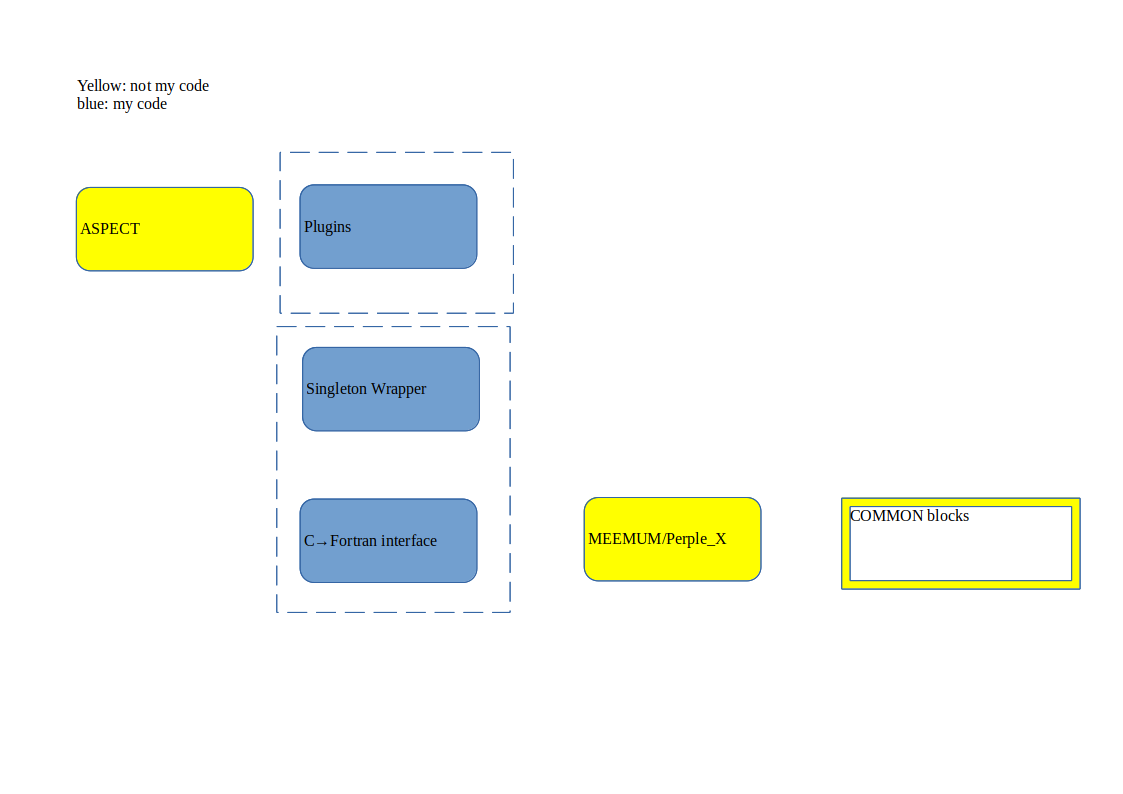
\includegraphics[width=\textwidth]{figures/dataflow.png}
    \caption{Diagram displaying the flow of data through the program. The blue blocks represent the new code and the yellow blocks represent the reused code.}
    \label{fig:dataflow}
\end{figure}

\subsection{Perple\_X C++ wrapper code}

The Perple\_X wrapper library presents two main functions to the user: one to initialise Perple\_X and the other to perform the MEEMUM computation and return the result.
It aims to abstract away to the greatest extent possible the complexities of dealing with the Perple\_X codebase.
For example, the only argument necessary to initialise the wrapper code is the path to the Perple\_X problem file and the only arguments needed to perform a subsequent calculation are the pressure, temperature and composition (which is just an array).

\subsubsection{Original Perple\_X source code}

Starting from the Perple\_X code and working up to the wrapper (see Figure~\ref{fig:dataflow}), the first component of the library is the Perple\_X source itself.
The decision was made to directly include the source code inside the repository rather than either encouraging the user to install Perple\_X themselves or retrieving via a URL.
The principle reason for this is reliability, Perple\_X receives frequent breaking updates and there is no easy way to access old versions so in order to ensure that the code remains in a usable state the source code is stored inside the repository.
The version used in the repository at the time of writing is 6.9.0.
Despite adding the code to the repository and tracking changes, the code has not been changed from the original Perple\_X code at all.
This is to try and minimise the amount of issues that will occur if at any point the Perple\_X version is ever upgraded.
Additionally the codebase is actually relatively small so inclusion does not create any significant overhead.
MEEMUM only depends on 8 (at the time of writing) source files and compilation occurs in well under a minute.

When Perple\_X is downloaded it comes with many files that compile to different executables other than MEEMUM as well as lots of thermodynamic database files and various README's.
To avoid confusion, only the necessary source files are included inside the repository.

\subsubsection{Fortran-to-C++ interface}

The basic concept of integrating Fortran code into C++ is very simple, all that is required is a C++ header file declaring the needed Fortran functions and variables using the correct symbols (e.g. the function \texttt{foo()} is normally represented with the symbol \texttt{foo\_} by the linker) and then the codes can be linked during compilation.
However, actually implementing this is far from straightforward: many of the data types are incompatible, array indexing starts from zero (C++) or one (Fortran) and arrays themselves are alternately row-major order (C++) and column-major order (Fortran).

This problem is compounded in Perple\_X by the sheer number of global variables, both constant PARAMETER's and COMMON blocks that are used by the program.
The source code contains a 400 line file called \texttt{perplex\_parameters.h} that contains the program parameters as well as lots of frequently used COMMON blocks.
If one were to write a C++ wrapper then this file would need to be converted into a C++ header as well as any MEEMUM specific code.

This was the approach taken previously by ???. A Python script was written that `compiled' the Fortran parameter file into a C++ header permitting linking.

However, this approach has a number of serious drawbacks: (a) whenever Perple\_X is upgraded this script must be re-run (b) the process is complex and hard to debug in case errors occur (c) the resulting header file is hard to read.

To solve these issues, an additional Fortran file was included in the codebase to `sanitise' the interface.
It provides a small number of property getters and setters as well as a largely verbatim copy of the MEEMUM subroutine, only altered to eliminate any calls for user input and split into initialise (called once) and compute (called many times) sections.
Arguments are passed by value (C-like) and only single values are passed (excluding strings), avoiding any complexities involved with arrays.

An additional advantage of this approach is readability.
Being written in Fortran 77, Perple\_X has a 6 character limit on its variable names which can make it very hard to follow what the variables and functions do.
The new interface code was not so restricted allowing for much more verbose function names.

\subsubsection{Singleton wrapper}

Although the basic interface described above is a significant improvement on previous approaches, it is still fairly limited.
Only basic data types are accepted and its use requires interacting with global variables, something that is considered poor software development practice.

Our solution to both these problems is the creation of a \texttt{Wrapper} class.
The class presents initialise and compute methods to the user and hides the details of interfacing with the Fortran at all.
It additionally permits the use of more complex data types, such as \texttt{std::vector} and \texttt{std::string} that are in common use in ASPECT.
An object-oriented solution was chosen because Perple\_X consists of both functions and data, making it a good idea to group them together into a class.

The class also implements the \textit{singleton pattern}, that is, only a single instance of the class may ever exist at the same time.
This approach was taken in order to prevent concurrent accesses to the Perple\_X data structures that are global.

During the project, it was noticed that many computations were being done with either identical or almost identical inputs. 
It therefore made sense to store the most frequently used results and use them if the inputs are sufficiently similar.
A cache was implemented using a least recently used (LRU) eviction policy.
A flowchart detailing the decision process for a LRU cache is shown in Figure~\ref{fig:cache_flowchart}.

\begin{figure}[ht]
    \centering
    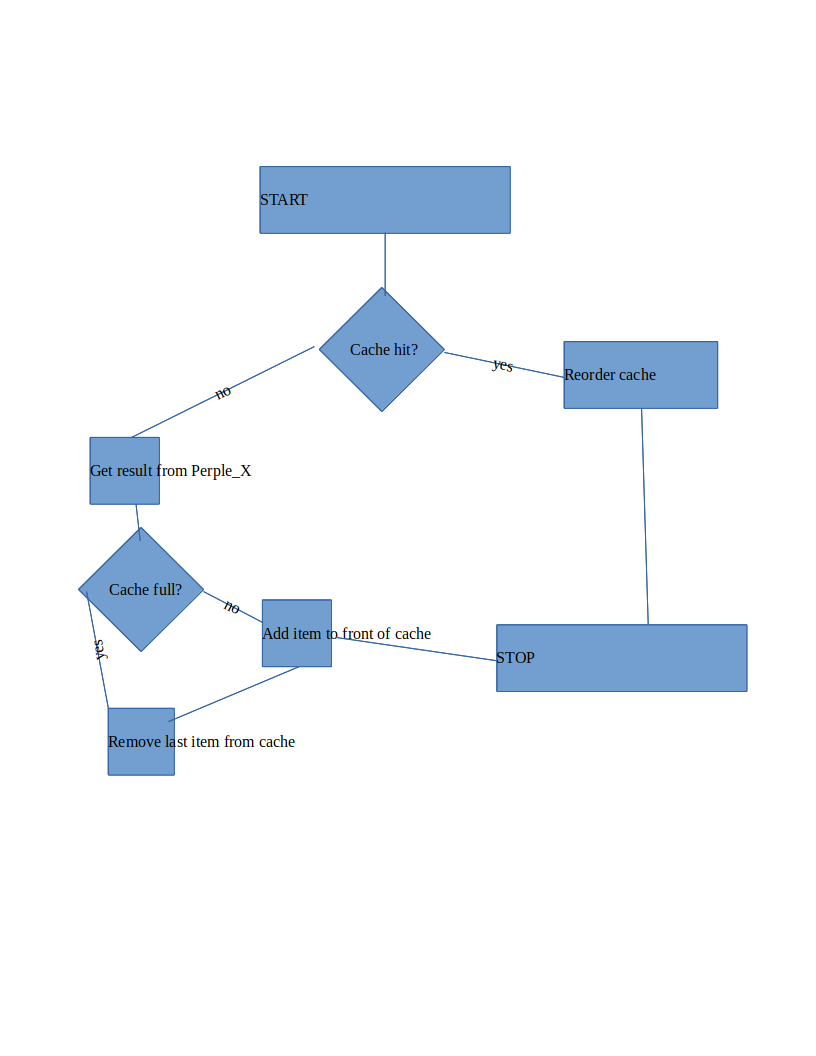
\includegraphics[width=\columnwidth]{./figures/cache_flowchart.png}
    \caption{Flowchart showing the decision process for the least recently used (LRU) cache used by the \texttt{Wrapper} class.}
    \label{fig:cache_flowchart}
\end{figure}

\subsubsection{Testing}

The library is tested using the Google C++ unit testing framework Google Test.
For the Fortran-to-C++ interface and singleton wrapper class, the tests consist largely of a direct comparison between the results of the function calls and previously collected MEEMUM output for a quick-to-run sample data set.

\subsubsection{Parallelism}

Perple\_X is not designed for parallel execution and as such the library is not thread-safe. 
However, there are only several methods that are exposed to the user so it would be straightforward to add locks to these methods making them thread-safe.
In contrast, the code is entirely suitable for parallel use in a distributed memory environment (i.e. MPI) because the global state is still local to each processor.
MPI is the primary parallelisation method used within ASPECT and so thread-safety was not considered a necessary feature of the library.

\subsection{ASPECT plugins}

The Perple\_X wrapper code was integrated into ASPECT using ASPECT's powerful plugin system.
Plugins are compiled into shared libraries with CMake.
These are libraries that are linked to at runtime, rather than compile time which is for static libraries.
Although care must be taken to use the same compiler for the plugin as for the main ASPECT binary this approach has significant advantage that it does not require recompilation of the main ASPECT binary every time.

The decision was taken to implement the code using the plugin system rather than forking the main ASPECT repository for the following reasons: 
(a) updating ASPECT does not require either rebasing or merging the git repositories 
(b) not having the new code mixed in with the original code makes things clearer 
(c) the code is rather specialist and may not ultimately be added to the ASPECT codebase.

The plugins expose to the user a set of options that may be included in the parameter file that is submitted to ASPECT.
Given the small number of source files that are written, no automatic method of generating the documentation has been written and we recommend reading the source code for parameter details.

Some example parameter files are included in the \texttt{cookbooks} component of the repository.
These provide examples of the various functionality of the plugins.

Regarding the actual plugins that were written, two different approaches were taken to track the Perple\_X composition in ASPECT: compositional fields (via a material model) and particles.
The details of their implementation will be discussed next.

\subsubsection{Particle plugin}

As discussed in Section~\ref{sec:introduction}, the basic idea of particles in a geodynamical simulation is that they are point objects passively advected around the medium with the velocity field.
At set timesteps they are then `evaluated' using the state of the different fields present at their current position.
In this work, a \textit{particle property} plugin was written that returns phase information from Perple\_X using the pressure, temperature, and, at least initially, bulk composition from the specified Perple\_X problem file.

The precise information that the plugin reports depends upon the options specified in the parameter file.
At present the possible properties that may be reported by the plugin for each endmember phase are the: composition, molar amount (in moles), molar fraction, volume fraction, and weight fraction.
This list would be straightforward to extend to any of the properties reported as output from MEEMUM and serves mainly as a proof-of-concept.

One particularly noteworthy set of options permitted by the plugin are \texttt{Extract melt} and \texttt{Melt extraction threshold}.
These permit an investigation of fractional melting of the material (see Section~\ref{sec:introduction} for a discussion of this).
If \texttt{Extract melt} is set to \texttt{true} then the particle will automatically report on the amount of moles of the melt that is extracted and on its composition.
Fractional properties (e.g. weight fraction) of the extracted melt are not tracked due to being non-physical.

\subsubsection{Material model plugin}

The ability to easily control the number of particles and evaluation rate is extremely useful for investigations with MEEMUM because each evaluation can take a considerable amount of time to complete.
The approach additionally permits the use of any material model.

However, it was found that the particle-based approach was incompatible with a study of two-phase flow.
This is because two-phase flow requires that the composition of the melt be advected separately to the composition of the residue.
In ASPECT particles can be set to \textit{either} advect with the melt field or with the solid material, but not both.
The underlying implementation of particles in ASPECT does not permit them to be differentiated into different classes.
Therefore there would be no way to use particles in a study of two-phase flow without a radical change to the ASPECT source code.

In this work we avoided this problem by pivoting to a compositional field-based approach and implementing a material model plugin.
In the simulation there are compositional fields for each component in the composition for both the melt and residue and these fields advect with either the solid or melt.

An unfortunate downside to this approach is that the parameter files become significantly more complex as the compositional fields must be specified by name and must correspond exactly to the compounds specified in the Perple\_X problem file.

The first material model plugin to be implemented used the ASPECT model \texttt{melt simple} as the underlying base model with some logic for calling MEEMUM and updating the relevant compositional fields on top.
This simplified development and ensured that any results from the simulation would be physically reasonable but had a significant downside in that the actual fraction of melt that was reported came from a simple parametrisation rather than from the composition-aware MEEMUM computation.
This not only makes the results less accurate, but it causes inconsistencies in the results such as when, for example, the ASPECT function reports the presence of melt but Perple\_X does not. 
In this situation the melt is reported as having no composition.

In an effort to mitigate the amount of disparity between the two models, the temperature being passed to Perple\_X is increased by $200 \mathrm{K}$.
This obviously impacts upon how reasonable the results can be considered to be.

To try and fix these issues, a material model that calculates the melt fraction using Perple\_X was also created.
However, the code experienced serious convergence issues and we ran out of time.
The code (\texttt{perplex\_melt.cc}) is included in the repository should anyone wish to get it working in future.

\subsubsection{Additional plugins}

In addition to the plugins discussed above, \textit{postprocessor} and \textit{initial composition} plugins were also written.
The postprocessor plugin is called \texttt{perplex cache statistics} and it permits analysis of the cache in the Perple\_X wrapper.
The initial composition plugin is called \texttt{perplex composition} and it makes sure that the compositional fields representing the melt and residue compositions (for two-phase flow) are initialised correctly.

\subsubsection{Testing}

Unit testing is difficult to do in ASPECT, as evidenced by the fact that very few actually exist in the main repository, due to the fact that plugins are tightly integrated with the rest of the simulation.
Most plugins inherit from the \texttt{SimulatorAccess} class in order to access information from the rest of the simulation such as time step number or to interact with other plugins.
Such complex interactions make typical unit testing of single pieces of functionality practically impossible.

Instead of using unit tests, ASPECT relies upon \textit{benchmarks} for evidence of its accuracy.
These involve running simulations with a known answer, for example the temperature change over a phase transition, and verifying that the ASPECT code converges to the correct answer.
The decision was made to not include any benchmarks with the code because they require detailed domain-specific knowledge and we were running out of time.

The other form of tests used in ASPECT simply compares the output of a simulation with a previous run to ensure that the results are unchanged.
Tests of this nature were not included in the code because the CMake script necessary to perform such a test is complex and we were limited by time.


\section{Results}
\label{sec:results}
\begin{table}[]
    \centering
    \begin{tabular}{c|c|c}
        Model & Decompression event & Closed box  \\
        Width ($\mathrm{km}$) & 1 & 300 \\
        Height ($\mathrm{km}$) & 120 & 120 \\
         & 
    \end{tabular}
    \caption{Caption}
    \label{tab:decompression_params}
\end{table}

\begin{figure}
    \centering
    %% Creator: Matplotlib, PGF backend
%%
%% To include the figure in your LaTeX document, write
%%   \input{<filename>.pgf}
%%
%% Make sure the required packages are loaded in your preamble
%%   \usepackage{pgf}
%%
%% Figures using additional raster images can only be included by \input if
%% they are in the same directory as the main LaTeX file. For loading figures
%% from other directories you can use the `import` package
%%   \usepackage{import}
%% and then include the figures with
%%   \import{<path to file>}{<filename>.pgf}
%%
%% Matplotlib used the following preamble
%%   \usepackage{fontspec}
%%   \setmainfont{DejaVuSerif.ttf}[Path=/home/connor/.local/lib/python3.8/site-packages/matplotlib/mpl-data/fonts/ttf/]
%%   \setsansfont{DejaVuSans.ttf}[Path=/home/connor/.local/lib/python3.8/site-packages/matplotlib/mpl-data/fonts/ttf/]
%%   \setmonofont{DejaVuSansMono.ttf}[Path=/home/connor/.local/lib/python3.8/site-packages/matplotlib/mpl-data/fonts/ttf/]
%%
\begingroup%
\makeatletter%
\begin{pgfpicture}%
\pgfpathrectangle{\pgfpointorigin}{\pgfqpoint{4.004230in}{3.132284in}}%
\pgfusepath{use as bounding box, clip}%
\begin{pgfscope}%
\pgfsetbuttcap%
\pgfsetmiterjoin%
\definecolor{currentfill}{rgb}{1.000000,1.000000,1.000000}%
\pgfsetfillcolor{currentfill}%
\pgfsetlinewidth{0.000000pt}%
\definecolor{currentstroke}{rgb}{1.000000,1.000000,1.000000}%
\pgfsetstrokecolor{currentstroke}%
\pgfsetdash{}{0pt}%
\pgfpathmoveto{\pgfqpoint{0.000000in}{0.000000in}}%
\pgfpathlineto{\pgfqpoint{4.004230in}{0.000000in}}%
\pgfpathlineto{\pgfqpoint{4.004230in}{3.132284in}}%
\pgfpathlineto{\pgfqpoint{0.000000in}{3.132284in}}%
\pgfpathclose%
\pgfusepath{fill}%
\end{pgfscope}%
\begin{pgfscope}%
\pgfsetbuttcap%
\pgfsetmiterjoin%
\definecolor{currentfill}{rgb}{1.000000,1.000000,1.000000}%
\pgfsetfillcolor{currentfill}%
\pgfsetlinewidth{0.000000pt}%
\definecolor{currentstroke}{rgb}{0.000000,0.000000,0.000000}%
\pgfsetstrokecolor{currentstroke}%
\pgfsetstrokeopacity{0.000000}%
\pgfsetdash{}{0pt}%
\pgfpathmoveto{\pgfqpoint{0.511159in}{1.741813in}}%
\pgfpathlineto{\pgfqpoint{3.904230in}{1.741813in}}%
\pgfpathlineto{\pgfqpoint{3.904230in}{3.014215in}}%
\pgfpathlineto{\pgfqpoint{0.511159in}{3.014215in}}%
\pgfpathclose%
\pgfusepath{fill}%
\end{pgfscope}%
\begin{pgfscope}%
\pgfsetbuttcap%
\pgfsetroundjoin%
\definecolor{currentfill}{rgb}{0.000000,0.000000,0.000000}%
\pgfsetfillcolor{currentfill}%
\pgfsetlinewidth{0.803000pt}%
\definecolor{currentstroke}{rgb}{0.000000,0.000000,0.000000}%
\pgfsetstrokecolor{currentstroke}%
\pgfsetdash{}{0pt}%
\pgfsys@defobject{currentmarker}{\pgfqpoint{0.000000in}{-0.048611in}}{\pgfqpoint{0.000000in}{0.000000in}}{%
\pgfpathmoveto{\pgfqpoint{0.000000in}{0.000000in}}%
\pgfpathlineto{\pgfqpoint{0.000000in}{-0.048611in}}%
\pgfusepath{stroke,fill}%
}%
\begin{pgfscope}%
\pgfsys@transformshift{0.665390in}{1.741813in}%
\pgfsys@useobject{currentmarker}{}%
\end{pgfscope}%
\end{pgfscope}%
\begin{pgfscope}%
\definecolor{textcolor}{rgb}{0.000000,0.000000,0.000000}%
\pgfsetstrokecolor{textcolor}%
\pgfsetfillcolor{textcolor}%
\pgftext[x=0.665390in,y=1.644591in,,top]{\color{textcolor}\rmfamily\fontsize{8.000000}{9.600000}\selectfont \(\displaystyle 0\)}%
\end{pgfscope}%
\begin{pgfscope}%
\pgfsetbuttcap%
\pgfsetroundjoin%
\definecolor{currentfill}{rgb}{0.000000,0.000000,0.000000}%
\pgfsetfillcolor{currentfill}%
\pgfsetlinewidth{0.803000pt}%
\definecolor{currentstroke}{rgb}{0.000000,0.000000,0.000000}%
\pgfsetstrokecolor{currentstroke}%
\pgfsetdash{}{0pt}%
\pgfsys@defobject{currentmarker}{\pgfqpoint{0.000000in}{-0.048611in}}{\pgfqpoint{0.000000in}{0.000000in}}{%
\pgfpathmoveto{\pgfqpoint{0.000000in}{0.000000in}}%
\pgfpathlineto{\pgfqpoint{0.000000in}{-0.048611in}}%
\pgfusepath{stroke,fill}%
}%
\begin{pgfscope}%
\pgfsys@transformshift{1.078738in}{1.741813in}%
\pgfsys@useobject{currentmarker}{}%
\end{pgfscope}%
\end{pgfscope}%
\begin{pgfscope}%
\definecolor{textcolor}{rgb}{0.000000,0.000000,0.000000}%
\pgfsetstrokecolor{textcolor}%
\pgfsetfillcolor{textcolor}%
\pgftext[x=1.078738in,y=1.644591in,,top]{\color{textcolor}\rmfamily\fontsize{8.000000}{9.600000}\selectfont \(\displaystyle 20000\)}%
\end{pgfscope}%
\begin{pgfscope}%
\pgfsetbuttcap%
\pgfsetroundjoin%
\definecolor{currentfill}{rgb}{0.000000,0.000000,0.000000}%
\pgfsetfillcolor{currentfill}%
\pgfsetlinewidth{0.803000pt}%
\definecolor{currentstroke}{rgb}{0.000000,0.000000,0.000000}%
\pgfsetstrokecolor{currentstroke}%
\pgfsetdash{}{0pt}%
\pgfsys@defobject{currentmarker}{\pgfqpoint{0.000000in}{-0.048611in}}{\pgfqpoint{0.000000in}{0.000000in}}{%
\pgfpathmoveto{\pgfqpoint{0.000000in}{0.000000in}}%
\pgfpathlineto{\pgfqpoint{0.000000in}{-0.048611in}}%
\pgfusepath{stroke,fill}%
}%
\begin{pgfscope}%
\pgfsys@transformshift{1.492086in}{1.741813in}%
\pgfsys@useobject{currentmarker}{}%
\end{pgfscope}%
\end{pgfscope}%
\begin{pgfscope}%
\definecolor{textcolor}{rgb}{0.000000,0.000000,0.000000}%
\pgfsetstrokecolor{textcolor}%
\pgfsetfillcolor{textcolor}%
\pgftext[x=1.492086in,y=1.644591in,,top]{\color{textcolor}\rmfamily\fontsize{8.000000}{9.600000}\selectfont \(\displaystyle 40000\)}%
\end{pgfscope}%
\begin{pgfscope}%
\pgfsetbuttcap%
\pgfsetroundjoin%
\definecolor{currentfill}{rgb}{0.000000,0.000000,0.000000}%
\pgfsetfillcolor{currentfill}%
\pgfsetlinewidth{0.803000pt}%
\definecolor{currentstroke}{rgb}{0.000000,0.000000,0.000000}%
\pgfsetstrokecolor{currentstroke}%
\pgfsetdash{}{0pt}%
\pgfsys@defobject{currentmarker}{\pgfqpoint{0.000000in}{-0.048611in}}{\pgfqpoint{0.000000in}{0.000000in}}{%
\pgfpathmoveto{\pgfqpoint{0.000000in}{0.000000in}}%
\pgfpathlineto{\pgfqpoint{0.000000in}{-0.048611in}}%
\pgfusepath{stroke,fill}%
}%
\begin{pgfscope}%
\pgfsys@transformshift{1.905434in}{1.741813in}%
\pgfsys@useobject{currentmarker}{}%
\end{pgfscope}%
\end{pgfscope}%
\begin{pgfscope}%
\definecolor{textcolor}{rgb}{0.000000,0.000000,0.000000}%
\pgfsetstrokecolor{textcolor}%
\pgfsetfillcolor{textcolor}%
\pgftext[x=1.905434in,y=1.644591in,,top]{\color{textcolor}\rmfamily\fontsize{8.000000}{9.600000}\selectfont \(\displaystyle 60000\)}%
\end{pgfscope}%
\begin{pgfscope}%
\pgfsetbuttcap%
\pgfsetroundjoin%
\definecolor{currentfill}{rgb}{0.000000,0.000000,0.000000}%
\pgfsetfillcolor{currentfill}%
\pgfsetlinewidth{0.803000pt}%
\definecolor{currentstroke}{rgb}{0.000000,0.000000,0.000000}%
\pgfsetstrokecolor{currentstroke}%
\pgfsetdash{}{0pt}%
\pgfsys@defobject{currentmarker}{\pgfqpoint{0.000000in}{-0.048611in}}{\pgfqpoint{0.000000in}{0.000000in}}{%
\pgfpathmoveto{\pgfqpoint{0.000000in}{0.000000in}}%
\pgfpathlineto{\pgfqpoint{0.000000in}{-0.048611in}}%
\pgfusepath{stroke,fill}%
}%
\begin{pgfscope}%
\pgfsys@transformshift{2.318782in}{1.741813in}%
\pgfsys@useobject{currentmarker}{}%
\end{pgfscope}%
\end{pgfscope}%
\begin{pgfscope}%
\definecolor{textcolor}{rgb}{0.000000,0.000000,0.000000}%
\pgfsetstrokecolor{textcolor}%
\pgfsetfillcolor{textcolor}%
\pgftext[x=2.318782in,y=1.644591in,,top]{\color{textcolor}\rmfamily\fontsize{8.000000}{9.600000}\selectfont \(\displaystyle 80000\)}%
\end{pgfscope}%
\begin{pgfscope}%
\pgfsetbuttcap%
\pgfsetroundjoin%
\definecolor{currentfill}{rgb}{0.000000,0.000000,0.000000}%
\pgfsetfillcolor{currentfill}%
\pgfsetlinewidth{0.803000pt}%
\definecolor{currentstroke}{rgb}{0.000000,0.000000,0.000000}%
\pgfsetstrokecolor{currentstroke}%
\pgfsetdash{}{0pt}%
\pgfsys@defobject{currentmarker}{\pgfqpoint{0.000000in}{-0.048611in}}{\pgfqpoint{0.000000in}{0.000000in}}{%
\pgfpathmoveto{\pgfqpoint{0.000000in}{0.000000in}}%
\pgfpathlineto{\pgfqpoint{0.000000in}{-0.048611in}}%
\pgfusepath{stroke,fill}%
}%
\begin{pgfscope}%
\pgfsys@transformshift{2.732130in}{1.741813in}%
\pgfsys@useobject{currentmarker}{}%
\end{pgfscope}%
\end{pgfscope}%
\begin{pgfscope}%
\definecolor{textcolor}{rgb}{0.000000,0.000000,0.000000}%
\pgfsetstrokecolor{textcolor}%
\pgfsetfillcolor{textcolor}%
\pgftext[x=2.732130in,y=1.644591in,,top]{\color{textcolor}\rmfamily\fontsize{8.000000}{9.600000}\selectfont \(\displaystyle 100000\)}%
\end{pgfscope}%
\begin{pgfscope}%
\pgfsetbuttcap%
\pgfsetroundjoin%
\definecolor{currentfill}{rgb}{0.000000,0.000000,0.000000}%
\pgfsetfillcolor{currentfill}%
\pgfsetlinewidth{0.803000pt}%
\definecolor{currentstroke}{rgb}{0.000000,0.000000,0.000000}%
\pgfsetstrokecolor{currentstroke}%
\pgfsetdash{}{0pt}%
\pgfsys@defobject{currentmarker}{\pgfqpoint{0.000000in}{-0.048611in}}{\pgfqpoint{0.000000in}{0.000000in}}{%
\pgfpathmoveto{\pgfqpoint{0.000000in}{0.000000in}}%
\pgfpathlineto{\pgfqpoint{0.000000in}{-0.048611in}}%
\pgfusepath{stroke,fill}%
}%
\begin{pgfscope}%
\pgfsys@transformshift{3.145478in}{1.741813in}%
\pgfsys@useobject{currentmarker}{}%
\end{pgfscope}%
\end{pgfscope}%
\begin{pgfscope}%
\definecolor{textcolor}{rgb}{0.000000,0.000000,0.000000}%
\pgfsetstrokecolor{textcolor}%
\pgfsetfillcolor{textcolor}%
\pgftext[x=3.145478in,y=1.644591in,,top]{\color{textcolor}\rmfamily\fontsize{8.000000}{9.600000}\selectfont \(\displaystyle 120000\)}%
\end{pgfscope}%
\begin{pgfscope}%
\pgfsetbuttcap%
\pgfsetroundjoin%
\definecolor{currentfill}{rgb}{0.000000,0.000000,0.000000}%
\pgfsetfillcolor{currentfill}%
\pgfsetlinewidth{0.803000pt}%
\definecolor{currentstroke}{rgb}{0.000000,0.000000,0.000000}%
\pgfsetstrokecolor{currentstroke}%
\pgfsetdash{}{0pt}%
\pgfsys@defobject{currentmarker}{\pgfqpoint{0.000000in}{-0.048611in}}{\pgfqpoint{0.000000in}{0.000000in}}{%
\pgfpathmoveto{\pgfqpoint{0.000000in}{0.000000in}}%
\pgfpathlineto{\pgfqpoint{0.000000in}{-0.048611in}}%
\pgfusepath{stroke,fill}%
}%
\begin{pgfscope}%
\pgfsys@transformshift{3.558826in}{1.741813in}%
\pgfsys@useobject{currentmarker}{}%
\end{pgfscope}%
\end{pgfscope}%
\begin{pgfscope}%
\definecolor{textcolor}{rgb}{0.000000,0.000000,0.000000}%
\pgfsetstrokecolor{textcolor}%
\pgfsetfillcolor{textcolor}%
\pgftext[x=3.558826in,y=1.644591in,,top]{\color{textcolor}\rmfamily\fontsize{8.000000}{9.600000}\selectfont \(\displaystyle 140000\)}%
\end{pgfscope}%
\begin{pgfscope}%
\pgfsetbuttcap%
\pgfsetroundjoin%
\definecolor{currentfill}{rgb}{0.000000,0.000000,0.000000}%
\pgfsetfillcolor{currentfill}%
\pgfsetlinewidth{0.803000pt}%
\definecolor{currentstroke}{rgb}{0.000000,0.000000,0.000000}%
\pgfsetstrokecolor{currentstroke}%
\pgfsetdash{}{0pt}%
\pgfsys@defobject{currentmarker}{\pgfqpoint{-0.048611in}{0.000000in}}{\pgfqpoint{0.000000in}{0.000000in}}{%
\pgfpathmoveto{\pgfqpoint{0.000000in}{0.000000in}}%
\pgfpathlineto{\pgfqpoint{-0.048611in}{0.000000in}}%
\pgfusepath{stroke,fill}%
}%
\begin{pgfscope}%
\pgfsys@transformshift{0.511159in}{1.799650in}%
\pgfsys@useobject{currentmarker}{}%
\end{pgfscope}%
\end{pgfscope}%
\begin{pgfscope}%
\definecolor{textcolor}{rgb}{0.000000,0.000000,0.000000}%
\pgfsetstrokecolor{textcolor}%
\pgfsetfillcolor{textcolor}%
\pgftext[x=0.263086in,y=1.757440in,left,base]{\color{textcolor}\rmfamily\fontsize{8.000000}{9.600000}\selectfont \(\displaystyle 0.0\)}%
\end{pgfscope}%
\begin{pgfscope}%
\pgfsetbuttcap%
\pgfsetroundjoin%
\definecolor{currentfill}{rgb}{0.000000,0.000000,0.000000}%
\pgfsetfillcolor{currentfill}%
\pgfsetlinewidth{0.803000pt}%
\definecolor{currentstroke}{rgb}{0.000000,0.000000,0.000000}%
\pgfsetstrokecolor{currentstroke}%
\pgfsetdash{}{0pt}%
\pgfsys@defobject{currentmarker}{\pgfqpoint{-0.048611in}{0.000000in}}{\pgfqpoint{0.000000in}{0.000000in}}{%
\pgfpathmoveto{\pgfqpoint{0.000000in}{0.000000in}}%
\pgfpathlineto{\pgfqpoint{-0.048611in}{0.000000in}}%
\pgfusepath{stroke,fill}%
}%
\begin{pgfscope}%
\pgfsys@transformshift{0.511159in}{2.070813in}%
\pgfsys@useobject{currentmarker}{}%
\end{pgfscope}%
\end{pgfscope}%
\begin{pgfscope}%
\definecolor{textcolor}{rgb}{0.000000,0.000000,0.000000}%
\pgfsetstrokecolor{textcolor}%
\pgfsetfillcolor{textcolor}%
\pgftext[x=0.263086in,y=2.028604in,left,base]{\color{textcolor}\rmfamily\fontsize{8.000000}{9.600000}\selectfont \(\displaystyle 0.5\)}%
\end{pgfscope}%
\begin{pgfscope}%
\pgfsetbuttcap%
\pgfsetroundjoin%
\definecolor{currentfill}{rgb}{0.000000,0.000000,0.000000}%
\pgfsetfillcolor{currentfill}%
\pgfsetlinewidth{0.803000pt}%
\definecolor{currentstroke}{rgb}{0.000000,0.000000,0.000000}%
\pgfsetstrokecolor{currentstroke}%
\pgfsetdash{}{0pt}%
\pgfsys@defobject{currentmarker}{\pgfqpoint{-0.048611in}{0.000000in}}{\pgfqpoint{0.000000in}{0.000000in}}{%
\pgfpathmoveto{\pgfqpoint{0.000000in}{0.000000in}}%
\pgfpathlineto{\pgfqpoint{-0.048611in}{0.000000in}}%
\pgfusepath{stroke,fill}%
}%
\begin{pgfscope}%
\pgfsys@transformshift{0.511159in}{2.341976in}%
\pgfsys@useobject{currentmarker}{}%
\end{pgfscope}%
\end{pgfscope}%
\begin{pgfscope}%
\definecolor{textcolor}{rgb}{0.000000,0.000000,0.000000}%
\pgfsetstrokecolor{textcolor}%
\pgfsetfillcolor{textcolor}%
\pgftext[x=0.263086in,y=2.299767in,left,base]{\color{textcolor}\rmfamily\fontsize{8.000000}{9.600000}\selectfont \(\displaystyle 1.0\)}%
\end{pgfscope}%
\begin{pgfscope}%
\pgfsetbuttcap%
\pgfsetroundjoin%
\definecolor{currentfill}{rgb}{0.000000,0.000000,0.000000}%
\pgfsetfillcolor{currentfill}%
\pgfsetlinewidth{0.803000pt}%
\definecolor{currentstroke}{rgb}{0.000000,0.000000,0.000000}%
\pgfsetstrokecolor{currentstroke}%
\pgfsetdash{}{0pt}%
\pgfsys@defobject{currentmarker}{\pgfqpoint{-0.048611in}{0.000000in}}{\pgfqpoint{0.000000in}{0.000000in}}{%
\pgfpathmoveto{\pgfqpoint{0.000000in}{0.000000in}}%
\pgfpathlineto{\pgfqpoint{-0.048611in}{0.000000in}}%
\pgfusepath{stroke,fill}%
}%
\begin{pgfscope}%
\pgfsys@transformshift{0.511159in}{2.613140in}%
\pgfsys@useobject{currentmarker}{}%
\end{pgfscope}%
\end{pgfscope}%
\begin{pgfscope}%
\definecolor{textcolor}{rgb}{0.000000,0.000000,0.000000}%
\pgfsetstrokecolor{textcolor}%
\pgfsetfillcolor{textcolor}%
\pgftext[x=0.263086in,y=2.570931in,left,base]{\color{textcolor}\rmfamily\fontsize{8.000000}{9.600000}\selectfont \(\displaystyle 1.5\)}%
\end{pgfscope}%
\begin{pgfscope}%
\pgfsetbuttcap%
\pgfsetroundjoin%
\definecolor{currentfill}{rgb}{0.000000,0.000000,0.000000}%
\pgfsetfillcolor{currentfill}%
\pgfsetlinewidth{0.803000pt}%
\definecolor{currentstroke}{rgb}{0.000000,0.000000,0.000000}%
\pgfsetstrokecolor{currentstroke}%
\pgfsetdash{}{0pt}%
\pgfsys@defobject{currentmarker}{\pgfqpoint{-0.048611in}{0.000000in}}{\pgfqpoint{0.000000in}{0.000000in}}{%
\pgfpathmoveto{\pgfqpoint{0.000000in}{0.000000in}}%
\pgfpathlineto{\pgfqpoint{-0.048611in}{0.000000in}}%
\pgfusepath{stroke,fill}%
}%
\begin{pgfscope}%
\pgfsys@transformshift{0.511159in}{2.884303in}%
\pgfsys@useobject{currentmarker}{}%
\end{pgfscope}%
\end{pgfscope}%
\begin{pgfscope}%
\definecolor{textcolor}{rgb}{0.000000,0.000000,0.000000}%
\pgfsetstrokecolor{textcolor}%
\pgfsetfillcolor{textcolor}%
\pgftext[x=0.263086in,y=2.842094in,left,base]{\color{textcolor}\rmfamily\fontsize{8.000000}{9.600000}\selectfont \(\displaystyle 2.0\)}%
\end{pgfscope}%
\begin{pgfscope}%
\definecolor{textcolor}{rgb}{0.000000,0.000000,0.000000}%
\pgfsetstrokecolor{textcolor}%
\pgfsetfillcolor{textcolor}%
\pgftext[x=0.207530in,y=2.378014in,,bottom,rotate=90.000000]{\color{textcolor}\rmfamily\fontsize{8.000000}{9.600000}\selectfont Melt composition (mol)}%
\end{pgfscope}%
\begin{pgfscope}%
\pgfpathrectangle{\pgfqpoint{0.511159in}{1.741813in}}{\pgfqpoint{3.393071in}{1.272402in}}%
\pgfusepath{clip}%
\pgfsetrectcap%
\pgfsetroundjoin%
\pgfsetlinewidth{1.505625pt}%
\definecolor{currentstroke}{rgb}{0.121569,0.466667,0.705882}%
\pgfsetstrokecolor{currentstroke}%
\pgfsetdash{}{0pt}%
\pgfpathmoveto{\pgfqpoint{0.665390in}{1.799650in}}%
\pgfpathlineto{\pgfqpoint{1.393916in}{1.799650in}}%
\pgfpathlineto{\pgfqpoint{1.414583in}{1.825296in}}%
\pgfpathlineto{\pgfqpoint{1.435250in}{2.081757in}}%
\pgfpathlineto{\pgfqpoint{1.497253in}{2.081757in}}%
\pgfpathlineto{\pgfqpoint{1.517920in}{2.093059in}}%
\pgfpathlineto{\pgfqpoint{1.538587in}{2.091644in}}%
\pgfpathlineto{\pgfqpoint{1.559255in}{2.090939in}}%
\pgfpathlineto{\pgfqpoint{1.579922in}{2.081757in}}%
\pgfpathlineto{\pgfqpoint{1.600590in}{2.089529in}}%
\pgfpathlineto{\pgfqpoint{1.641924in}{2.086351in}}%
\pgfpathlineto{\pgfqpoint{1.662592in}{2.070461in}}%
\pgfpathlineto{\pgfqpoint{1.765929in}{2.070461in}}%
\pgfpathlineto{\pgfqpoint{1.786596in}{2.064810in}}%
\pgfpathlineto{\pgfqpoint{1.807264in}{2.070461in}}%
\pgfpathlineto{\pgfqpoint{1.848598in}{2.070461in}}%
\pgfpathlineto{\pgfqpoint{1.869266in}{2.068308in}}%
\pgfpathlineto{\pgfqpoint{1.889933in}{2.068340in}}%
\pgfpathlineto{\pgfqpoint{1.910601in}{2.064115in}}%
\pgfpathlineto{\pgfqpoint{1.931268in}{2.062808in}}%
\pgfpathlineto{\pgfqpoint{1.951935in}{2.059869in}}%
\pgfpathlineto{\pgfqpoint{1.972603in}{2.059869in}}%
\pgfpathlineto{\pgfqpoint{1.993270in}{2.057396in}}%
\pgfpathlineto{\pgfqpoint{2.075940in}{2.050687in}}%
\pgfpathlineto{\pgfqpoint{2.096607in}{2.047862in}}%
\pgfpathlineto{\pgfqpoint{2.117275in}{2.047412in}}%
\pgfpathlineto{\pgfqpoint{2.158609in}{2.042759in}}%
\pgfpathlineto{\pgfqpoint{2.179277in}{2.041506in}}%
\pgfpathlineto{\pgfqpoint{2.261946in}{2.030209in}}%
\pgfpathlineto{\pgfqpoint{2.282614in}{2.028799in}}%
\pgfpathlineto{\pgfqpoint{2.303281in}{2.026679in}}%
\pgfpathlineto{\pgfqpoint{2.323949in}{2.025572in}}%
\pgfpathlineto{\pgfqpoint{2.344616in}{2.023853in}}%
\pgfpathlineto{\pgfqpoint{2.406618in}{2.016087in}}%
\pgfpathlineto{\pgfqpoint{2.427286in}{2.014319in}}%
\pgfpathlineto{\pgfqpoint{2.489288in}{2.004215in}}%
\pgfpathlineto{\pgfqpoint{2.509955in}{2.003375in}}%
\pgfpathlineto{\pgfqpoint{2.551290in}{2.003375in}}%
\pgfpathlineto{\pgfqpoint{2.571958in}{1.997724in}}%
\pgfpathlineto{\pgfqpoint{2.592625in}{1.995961in}}%
\pgfpathlineto{\pgfqpoint{2.654627in}{1.986731in}}%
\pgfpathlineto{\pgfqpoint{2.675295in}{1.985245in}}%
\pgfpathlineto{\pgfqpoint{2.695962in}{1.982191in}}%
\pgfpathlineto{\pgfqpoint{2.716629in}{1.982099in}}%
\pgfpathlineto{\pgfqpoint{2.737297in}{1.983075in}}%
\pgfpathlineto{\pgfqpoint{2.757964in}{1.982186in}}%
\pgfpathlineto{\pgfqpoint{3.005973in}{1.982962in}}%
\pgfpathlineto{\pgfqpoint{3.150645in}{1.982897in}}%
\pgfpathlineto{\pgfqpoint{3.274649in}{1.983200in}}%
\pgfpathlineto{\pgfqpoint{3.315984in}{1.982897in}}%
\pgfpathlineto{\pgfqpoint{3.481323in}{1.982436in}}%
\pgfpathlineto{\pgfqpoint{3.605328in}{1.981774in}}%
\pgfpathlineto{\pgfqpoint{3.646662in}{1.982392in}}%
\pgfpathlineto{\pgfqpoint{3.667330in}{1.981503in}}%
\pgfpathlineto{\pgfqpoint{3.687997in}{1.981644in}}%
\pgfpathlineto{\pgfqpoint{3.708665in}{1.982436in}}%
\pgfpathlineto{\pgfqpoint{3.729332in}{1.981091in}}%
\pgfpathlineto{\pgfqpoint{3.750000in}{1.981053in}}%
\pgfpathlineto{\pgfqpoint{3.750000in}{1.981053in}}%
\pgfusepath{stroke}%
\end{pgfscope}%
\begin{pgfscope}%
\pgfpathrectangle{\pgfqpoint{0.511159in}{1.741813in}}{\pgfqpoint{3.393071in}{1.272402in}}%
\pgfusepath{clip}%
\pgfsetrectcap%
\pgfsetroundjoin%
\pgfsetlinewidth{1.505625pt}%
\definecolor{currentstroke}{rgb}{1.000000,0.498039,0.054902}%
\pgfsetstrokecolor{currentstroke}%
\pgfsetdash{}{0pt}%
\pgfpathmoveto{\pgfqpoint{0.665390in}{1.799650in}}%
\pgfpathlineto{\pgfqpoint{1.393916in}{1.799650in}}%
\pgfpathlineto{\pgfqpoint{1.414583in}{1.821605in}}%
\pgfpathlineto{\pgfqpoint{1.435250in}{2.039743in}}%
\pgfpathlineto{\pgfqpoint{1.455918in}{2.036918in}}%
\pgfpathlineto{\pgfqpoint{1.476585in}{2.032682in}}%
\pgfpathlineto{\pgfqpoint{1.497253in}{2.031267in}}%
\pgfpathlineto{\pgfqpoint{1.517920in}{2.024206in}}%
\pgfpathlineto{\pgfqpoint{1.538587in}{2.022795in}}%
\pgfpathlineto{\pgfqpoint{1.559255in}{2.022795in}}%
\pgfpathlineto{\pgfqpoint{1.579922in}{2.024206in}}%
\pgfpathlineto{\pgfqpoint{1.600590in}{2.021380in}}%
\pgfpathlineto{\pgfqpoint{1.641924in}{2.018560in}}%
\pgfpathlineto{\pgfqpoint{1.662592in}{2.021380in}}%
\pgfpathlineto{\pgfqpoint{1.724594in}{2.017144in}}%
\pgfpathlineto{\pgfqpoint{1.745261in}{2.014319in}}%
\pgfpathlineto{\pgfqpoint{1.786596in}{2.014319in}}%
\pgfpathlineto{\pgfqpoint{1.807264in}{2.011493in}}%
\pgfpathlineto{\pgfqpoint{1.848598in}{2.011493in}}%
\pgfpathlineto{\pgfqpoint{1.869266in}{2.008798in}}%
\pgfpathlineto{\pgfqpoint{1.889933in}{2.003022in}}%
\pgfpathlineto{\pgfqpoint{1.910601in}{2.011266in}}%
\pgfpathlineto{\pgfqpoint{1.931268in}{2.010083in}}%
\pgfpathlineto{\pgfqpoint{1.951935in}{2.010083in}}%
\pgfpathlineto{\pgfqpoint{1.972603in}{2.004432in}}%
\pgfpathlineto{\pgfqpoint{1.993270in}{2.004432in}}%
\pgfpathlineto{\pgfqpoint{2.013938in}{2.003022in}}%
\pgfpathlineto{\pgfqpoint{2.034605in}{2.003022in}}%
\pgfpathlineto{\pgfqpoint{2.055272in}{2.001612in}}%
\pgfpathlineto{\pgfqpoint{2.096607in}{2.001612in}}%
\pgfpathlineto{\pgfqpoint{2.137942in}{1.998787in}}%
\pgfpathlineto{\pgfqpoint{2.158609in}{1.998787in}}%
\pgfpathlineto{\pgfqpoint{2.179277in}{1.997707in}}%
\pgfpathlineto{\pgfqpoint{2.199944in}{1.997371in}}%
\pgfpathlineto{\pgfqpoint{2.261946in}{1.993136in}}%
\pgfpathlineto{\pgfqpoint{2.323949in}{1.992935in}}%
\pgfpathlineto{\pgfqpoint{2.365283in}{1.991026in}}%
\pgfpathlineto{\pgfqpoint{2.385951in}{1.990310in}}%
\pgfpathlineto{\pgfqpoint{2.406618in}{1.990310in}}%
\pgfpathlineto{\pgfqpoint{2.447953in}{1.988900in}}%
\pgfpathlineto{\pgfqpoint{2.489288in}{1.986617in}}%
\pgfpathlineto{\pgfqpoint{2.530623in}{1.984795in}}%
\pgfpathlineto{\pgfqpoint{2.571958in}{1.984220in}}%
\pgfpathlineto{\pgfqpoint{2.654627in}{1.980424in}}%
\pgfpathlineto{\pgfqpoint{2.675295in}{1.980277in}}%
\pgfpathlineto{\pgfqpoint{2.695962in}{1.979013in}}%
\pgfpathlineto{\pgfqpoint{2.737297in}{1.979333in}}%
\pgfpathlineto{\pgfqpoint{2.778632in}{1.981123in}}%
\pgfpathlineto{\pgfqpoint{2.819966in}{1.981150in}}%
\pgfpathlineto{\pgfqpoint{2.881969in}{1.983038in}}%
\pgfpathlineto{\pgfqpoint{2.943971in}{1.983249in}}%
\pgfpathlineto{\pgfqpoint{2.964638in}{1.984664in}}%
\pgfpathlineto{\pgfqpoint{3.005973in}{1.984968in}}%
\pgfpathlineto{\pgfqpoint{3.047308in}{1.986834in}}%
\pgfpathlineto{\pgfqpoint{3.067975in}{1.986839in}}%
\pgfpathlineto{\pgfqpoint{3.088643in}{1.987485in}}%
\pgfpathlineto{\pgfqpoint{3.109310in}{1.987485in}}%
\pgfpathlineto{\pgfqpoint{3.129977in}{1.988705in}}%
\pgfpathlineto{\pgfqpoint{3.171312in}{1.988900in}}%
\pgfpathlineto{\pgfqpoint{3.191980in}{1.990261in}}%
\pgfpathlineto{\pgfqpoint{3.233314in}{1.990310in}}%
\pgfpathlineto{\pgfqpoint{3.253982in}{1.991726in}}%
\pgfpathlineto{\pgfqpoint{3.274649in}{1.992105in}}%
\pgfpathlineto{\pgfqpoint{3.295317in}{1.993136in}}%
\pgfpathlineto{\pgfqpoint{3.315984in}{1.993136in}}%
\pgfpathlineto{\pgfqpoint{3.357319in}{1.994204in}}%
\pgfpathlineto{\pgfqpoint{3.439988in}{1.995961in}}%
\pgfpathlineto{\pgfqpoint{3.460656in}{1.997371in}}%
\pgfpathlineto{\pgfqpoint{3.501991in}{1.997458in}}%
\pgfpathlineto{\pgfqpoint{3.522658in}{1.999221in}}%
\pgfpathlineto{\pgfqpoint{3.563993in}{2.000728in}}%
\pgfpathlineto{\pgfqpoint{3.584660in}{2.000929in}}%
\pgfpathlineto{\pgfqpoint{3.605328in}{2.000197in}}%
\pgfpathlineto{\pgfqpoint{3.646662in}{1.997496in}}%
\pgfpathlineto{\pgfqpoint{3.667330in}{2.000929in}}%
\pgfpathlineto{\pgfqpoint{3.687997in}{2.002811in}}%
\pgfpathlineto{\pgfqpoint{3.708665in}{2.001612in}}%
\pgfpathlineto{\pgfqpoint{3.729332in}{2.002632in}}%
\pgfpathlineto{\pgfqpoint{3.750000in}{2.002616in}}%
\pgfpathlineto{\pgfqpoint{3.750000in}{2.002616in}}%
\pgfusepath{stroke}%
\end{pgfscope}%
\begin{pgfscope}%
\pgfpathrectangle{\pgfqpoint{0.511159in}{1.741813in}}{\pgfqpoint{3.393071in}{1.272402in}}%
\pgfusepath{clip}%
\pgfsetrectcap%
\pgfsetroundjoin%
\pgfsetlinewidth{1.505625pt}%
\definecolor{currentstroke}{rgb}{0.172549,0.627451,0.172549}%
\pgfsetstrokecolor{currentstroke}%
\pgfsetdash{}{0pt}%
\pgfpathmoveto{\pgfqpoint{0.665390in}{1.799650in}}%
\pgfpathlineto{\pgfqpoint{1.393916in}{1.799650in}}%
\pgfpathlineto{\pgfqpoint{1.414583in}{1.860379in}}%
\pgfpathlineto{\pgfqpoint{1.435250in}{2.467688in}}%
\pgfpathlineto{\pgfqpoint{1.476585in}{2.467688in}}%
\pgfpathlineto{\pgfqpoint{1.497253in}{2.466278in}}%
\pgfpathlineto{\pgfqpoint{1.517920in}{2.440843in}}%
\pgfpathlineto{\pgfqpoint{1.538587in}{2.443663in}}%
\pgfpathlineto{\pgfqpoint{1.559255in}{2.443663in}}%
\pgfpathlineto{\pgfqpoint{1.579922in}{2.464868in}}%
\pgfpathlineto{\pgfqpoint{1.600590in}{2.446483in}}%
\pgfpathlineto{\pgfqpoint{1.641924in}{2.452123in}}%
\pgfpathlineto{\pgfqpoint{1.662592in}{2.486018in}}%
\pgfpathlineto{\pgfqpoint{1.683259in}{2.486018in}}%
\pgfpathlineto{\pgfqpoint{1.703927in}{2.484608in}}%
\pgfpathlineto{\pgfqpoint{1.724594in}{2.481788in}}%
\pgfpathlineto{\pgfqpoint{1.745261in}{2.481788in}}%
\pgfpathlineto{\pgfqpoint{1.765929in}{2.478968in}}%
\pgfpathlineto{\pgfqpoint{1.786596in}{2.490249in}}%
\pgfpathlineto{\pgfqpoint{1.807264in}{2.476148in}}%
\pgfpathlineto{\pgfqpoint{1.827931in}{2.476148in}}%
\pgfpathlineto{\pgfqpoint{1.848598in}{2.473328in}}%
\pgfpathlineto{\pgfqpoint{1.869266in}{2.476148in}}%
\pgfpathlineto{\pgfqpoint{1.889933in}{2.477558in}}%
\pgfpathlineto{\pgfqpoint{1.910601in}{2.480378in}}%
\pgfpathlineto{\pgfqpoint{1.931268in}{2.481788in}}%
\pgfpathlineto{\pgfqpoint{1.951935in}{2.484608in}}%
\pgfpathlineto{\pgfqpoint{1.972603in}{2.486018in}}%
\pgfpathlineto{\pgfqpoint{2.034605in}{2.494479in}}%
\pgfpathlineto{\pgfqpoint{2.075940in}{2.497353in}}%
\pgfpathlineto{\pgfqpoint{2.096607in}{2.501583in}}%
\pgfpathlineto{\pgfqpoint{2.117275in}{2.500173in}}%
\pgfpathlineto{\pgfqpoint{2.137942in}{2.502993in}}%
\pgfpathlineto{\pgfqpoint{2.199944in}{2.508633in}}%
\pgfpathlineto{\pgfqpoint{2.220612in}{2.512864in}}%
\pgfpathlineto{\pgfqpoint{2.261946in}{2.518504in}}%
\pgfpathlineto{\pgfqpoint{2.282614in}{2.518504in}}%
\pgfpathlineto{\pgfqpoint{2.303281in}{2.521324in}}%
\pgfpathlineto{\pgfqpoint{2.323949in}{2.521541in}}%
\pgfpathlineto{\pgfqpoint{2.344616in}{2.522734in}}%
\pgfpathlineto{\pgfqpoint{2.385951in}{2.528428in}}%
\pgfpathlineto{\pgfqpoint{2.427286in}{2.531249in}}%
\pgfpathlineto{\pgfqpoint{2.489288in}{2.539166in}}%
\pgfpathlineto{\pgfqpoint{2.509955in}{2.537431in}}%
\pgfpathlineto{\pgfqpoint{2.530623in}{2.534448in}}%
\pgfpathlineto{\pgfqpoint{2.551290in}{2.532659in}}%
\pgfpathlineto{\pgfqpoint{2.571958in}{2.542963in}}%
\pgfpathlineto{\pgfqpoint{2.592625in}{2.545349in}}%
\pgfpathlineto{\pgfqpoint{2.633960in}{2.548169in}}%
\pgfpathlineto{\pgfqpoint{2.654627in}{2.550447in}}%
\pgfpathlineto{\pgfqpoint{2.675295in}{2.550989in}}%
\pgfpathlineto{\pgfqpoint{2.695962in}{2.552399in}}%
\pgfpathlineto{\pgfqpoint{2.716629in}{2.551369in}}%
\pgfpathlineto{\pgfqpoint{2.737297in}{2.544536in}}%
\pgfpathlineto{\pgfqpoint{2.757964in}{2.549579in}}%
\pgfpathlineto{\pgfqpoint{2.799299in}{2.546759in}}%
\pgfpathlineto{\pgfqpoint{2.819966in}{2.546759in}}%
\pgfpathlineto{\pgfqpoint{2.840634in}{2.545349in}}%
\pgfpathlineto{\pgfqpoint{2.861301in}{2.545349in}}%
\pgfpathlineto{\pgfqpoint{2.881969in}{2.543939in}}%
\pgfpathlineto{\pgfqpoint{2.902636in}{2.543939in}}%
\pgfpathlineto{\pgfqpoint{2.923303in}{2.542529in}}%
\pgfpathlineto{\pgfqpoint{2.943971in}{2.542529in}}%
\pgfpathlineto{\pgfqpoint{2.964638in}{2.541119in}}%
\pgfpathlineto{\pgfqpoint{2.985306in}{2.541119in}}%
\pgfpathlineto{\pgfqpoint{3.005973in}{2.539709in}}%
\pgfpathlineto{\pgfqpoint{3.047308in}{2.538299in}}%
\pgfpathlineto{\pgfqpoint{3.067975in}{2.538245in}}%
\pgfpathlineto{\pgfqpoint{3.088643in}{2.536889in}}%
\pgfpathlineto{\pgfqpoint{3.150645in}{2.536401in}}%
\pgfpathlineto{\pgfqpoint{3.171312in}{2.535479in}}%
\pgfpathlineto{\pgfqpoint{3.212647in}{2.535316in}}%
\pgfpathlineto{\pgfqpoint{3.233314in}{2.534069in}}%
\pgfpathlineto{\pgfqpoint{3.274649in}{2.534069in}}%
\pgfpathlineto{\pgfqpoint{3.295317in}{2.535099in}}%
\pgfpathlineto{\pgfqpoint{3.315984in}{2.535099in}}%
\pgfpathlineto{\pgfqpoint{3.357319in}{2.534069in}}%
\pgfpathlineto{\pgfqpoint{3.481323in}{2.534069in}}%
\pgfpathlineto{\pgfqpoint{3.501991in}{2.535208in}}%
\pgfpathlineto{\pgfqpoint{3.543325in}{2.535479in}}%
\pgfpathlineto{\pgfqpoint{3.563993in}{2.536889in}}%
\pgfpathlineto{\pgfqpoint{3.584660in}{2.536889in}}%
\pgfpathlineto{\pgfqpoint{3.625995in}{2.534286in}}%
\pgfpathlineto{\pgfqpoint{3.646662in}{2.534231in}}%
\pgfpathlineto{\pgfqpoint{3.667330in}{2.536889in}}%
\pgfpathlineto{\pgfqpoint{3.687997in}{2.534069in}}%
\pgfpathlineto{\pgfqpoint{3.708665in}{2.529838in}}%
\pgfpathlineto{\pgfqpoint{3.729332in}{2.538028in}}%
\pgfpathlineto{\pgfqpoint{3.750000in}{2.538299in}}%
\pgfpathlineto{\pgfqpoint{3.750000in}{2.538299in}}%
\pgfusepath{stroke}%
\end{pgfscope}%
\begin{pgfscope}%
\pgfpathrectangle{\pgfqpoint{0.511159in}{1.741813in}}{\pgfqpoint{3.393071in}{1.272402in}}%
\pgfusepath{clip}%
\pgfsetrectcap%
\pgfsetroundjoin%
\pgfsetlinewidth{1.505625pt}%
\definecolor{currentstroke}{rgb}{0.839216,0.152941,0.156863}%
\pgfsetstrokecolor{currentstroke}%
\pgfsetdash{}{0pt}%
\pgfpathmoveto{\pgfqpoint{0.665390in}{1.799650in}}%
\pgfpathlineto{\pgfqpoint{1.393916in}{1.799650in}}%
\pgfpathlineto{\pgfqpoint{1.414583in}{1.878580in}}%
\pgfpathlineto{\pgfqpoint{1.435250in}{2.668566in}}%
\pgfpathlineto{\pgfqpoint{1.455918in}{2.669976in}}%
\pgfpathlineto{\pgfqpoint{1.476585in}{2.672091in}}%
\pgfpathlineto{\pgfqpoint{1.497253in}{2.673501in}}%
\pgfpathlineto{\pgfqpoint{1.517920in}{2.655875in}}%
\pgfpathlineto{\pgfqpoint{1.538587in}{2.659400in}}%
\pgfpathlineto{\pgfqpoint{1.559255in}{2.661515in}}%
\pgfpathlineto{\pgfqpoint{1.579922in}{2.677731in}}%
\pgfpathlineto{\pgfqpoint{1.600590in}{2.665041in}}%
\pgfpathlineto{\pgfqpoint{1.621257in}{2.669650in}}%
\pgfpathlineto{\pgfqpoint{1.641924in}{2.673175in}}%
\pgfpathlineto{\pgfqpoint{1.662592in}{2.702461in}}%
\pgfpathlineto{\pgfqpoint{1.683259in}{2.703166in}}%
\pgfpathlineto{\pgfqpoint{1.703927in}{2.704576in}}%
\pgfpathlineto{\pgfqpoint{1.724594in}{2.706691in}}%
\pgfpathlineto{\pgfqpoint{1.765929in}{2.709511in}}%
\pgfpathlineto{\pgfqpoint{1.786596in}{2.720846in}}%
\pgfpathlineto{\pgfqpoint{1.807264in}{2.712331in}}%
\pgfpathlineto{\pgfqpoint{1.827931in}{2.712331in}}%
\pgfpathlineto{\pgfqpoint{1.848598in}{2.713741in}}%
\pgfpathlineto{\pgfqpoint{1.869266in}{2.720141in}}%
\pgfpathlineto{\pgfqpoint{1.889933in}{2.722256in}}%
\pgfpathlineto{\pgfqpoint{1.910601in}{2.729415in}}%
\pgfpathlineto{\pgfqpoint{1.931268in}{2.733211in}}%
\pgfpathlineto{\pgfqpoint{1.951935in}{2.740587in}}%
\pgfpathlineto{\pgfqpoint{1.972603in}{2.742702in}}%
\pgfpathlineto{\pgfqpoint{1.993270in}{2.748722in}}%
\pgfpathlineto{\pgfqpoint{2.055272in}{2.762497in}}%
\pgfpathlineto{\pgfqpoint{2.075940in}{2.766022in}}%
\pgfpathlineto{\pgfqpoint{2.096607in}{2.772367in}}%
\pgfpathlineto{\pgfqpoint{2.117275in}{2.775133in}}%
\pgfpathlineto{\pgfqpoint{2.158609in}{2.787389in}}%
\pgfpathlineto{\pgfqpoint{2.179277in}{2.790752in}}%
\pgfpathlineto{\pgfqpoint{2.199944in}{2.798507in}}%
\pgfpathlineto{\pgfqpoint{2.220612in}{2.807022in}}%
\pgfpathlineto{\pgfqpoint{2.241279in}{2.813313in}}%
\pgfpathlineto{\pgfqpoint{2.261946in}{2.821122in}}%
\pgfpathlineto{\pgfqpoint{2.282614in}{2.825352in}}%
\pgfpathlineto{\pgfqpoint{2.303281in}{2.830287in}}%
\pgfpathlineto{\pgfqpoint{2.323949in}{2.833596in}}%
\pgfpathlineto{\pgfqpoint{2.344616in}{2.838748in}}%
\pgfpathlineto{\pgfqpoint{2.365283in}{2.845418in}}%
\pgfpathlineto{\pgfqpoint{2.385951in}{2.853282in}}%
\pgfpathlineto{\pgfqpoint{2.406618in}{2.859248in}}%
\pgfpathlineto{\pgfqpoint{2.427286in}{2.864183in}}%
\pgfpathlineto{\pgfqpoint{2.468620in}{2.883436in}}%
\pgfpathlineto{\pgfqpoint{2.489288in}{2.892004in}}%
\pgfpathlineto{\pgfqpoint{2.509955in}{2.895963in}}%
\pgfpathlineto{\pgfqpoint{2.530623in}{2.897807in}}%
\pgfpathlineto{\pgfqpoint{2.551290in}{2.898783in}}%
\pgfpathlineto{\pgfqpoint{2.571958in}{2.910769in}}%
\pgfpathlineto{\pgfqpoint{2.592625in}{2.915379in}}%
\pgfpathlineto{\pgfqpoint{2.613292in}{2.924924in}}%
\pgfpathlineto{\pgfqpoint{2.654627in}{2.941898in}}%
\pgfpathlineto{\pgfqpoint{2.675295in}{2.946183in}}%
\pgfpathlineto{\pgfqpoint{2.695962in}{2.955294in}}%
\pgfpathlineto{\pgfqpoint{2.737297in}{2.956378in}}%
\pgfpathlineto{\pgfqpoint{2.778632in}{2.956053in}}%
\pgfpathlineto{\pgfqpoint{3.109310in}{2.956378in}}%
\pgfpathlineto{\pgfqpoint{3.171312in}{2.956378in}}%
\pgfpathlineto{\pgfqpoint{3.191980in}{2.954968in}}%
\pgfpathlineto{\pgfqpoint{3.605328in}{2.954263in}}%
\pgfpathlineto{\pgfqpoint{3.646662in}{2.954535in}}%
\pgfpathlineto{\pgfqpoint{3.687997in}{2.954209in}}%
\pgfpathlineto{\pgfqpoint{3.708665in}{2.954535in}}%
\pgfpathlineto{\pgfqpoint{3.729332in}{2.953938in}}%
\pgfpathlineto{\pgfqpoint{3.750000in}{2.953938in}}%
\pgfpathlineto{\pgfqpoint{3.750000in}{2.953938in}}%
\pgfusepath{stroke}%
\end{pgfscope}%
\begin{pgfscope}%
\pgfsetrectcap%
\pgfsetmiterjoin%
\pgfsetlinewidth{0.803000pt}%
\definecolor{currentstroke}{rgb}{0.000000,0.000000,0.000000}%
\pgfsetstrokecolor{currentstroke}%
\pgfsetdash{}{0pt}%
\pgfpathmoveto{\pgfqpoint{0.511159in}{1.741813in}}%
\pgfpathlineto{\pgfqpoint{0.511159in}{3.014215in}}%
\pgfusepath{stroke}%
\end{pgfscope}%
\begin{pgfscope}%
\pgfsetrectcap%
\pgfsetmiterjoin%
\pgfsetlinewidth{0.803000pt}%
\definecolor{currentstroke}{rgb}{0.000000,0.000000,0.000000}%
\pgfsetstrokecolor{currentstroke}%
\pgfsetdash{}{0pt}%
\pgfpathmoveto{\pgfqpoint{3.904230in}{1.741813in}}%
\pgfpathlineto{\pgfqpoint{3.904230in}{3.014215in}}%
\pgfusepath{stroke}%
\end{pgfscope}%
\begin{pgfscope}%
\pgfsetrectcap%
\pgfsetmiterjoin%
\pgfsetlinewidth{0.803000pt}%
\definecolor{currentstroke}{rgb}{0.000000,0.000000,0.000000}%
\pgfsetstrokecolor{currentstroke}%
\pgfsetdash{}{0pt}%
\pgfpathmoveto{\pgfqpoint{0.511159in}{1.741813in}}%
\pgfpathlineto{\pgfqpoint{3.904230in}{1.741813in}}%
\pgfusepath{stroke}%
\end{pgfscope}%
\begin{pgfscope}%
\pgfsetrectcap%
\pgfsetmiterjoin%
\pgfsetlinewidth{0.803000pt}%
\definecolor{currentstroke}{rgb}{0.000000,0.000000,0.000000}%
\pgfsetstrokecolor{currentstroke}%
\pgfsetdash{}{0pt}%
\pgfpathmoveto{\pgfqpoint{0.511159in}{3.014215in}}%
\pgfpathlineto{\pgfqpoint{3.904230in}{3.014215in}}%
\pgfusepath{stroke}%
\end{pgfscope}%
\begin{pgfscope}%
\pgfsetrectcap%
\pgfsetroundjoin%
\pgfsetlinewidth{1.505625pt}%
\definecolor{currentstroke}{rgb}{0.121569,0.466667,0.705882}%
\pgfsetstrokecolor{currentstroke}%
\pgfsetdash{}{0pt}%
\pgfpathmoveto{\pgfqpoint{0.611159in}{2.868685in}}%
\pgfpathlineto{\pgfqpoint{0.833381in}{2.868685in}}%
\pgfusepath{stroke}%
\end{pgfscope}%
\begin{pgfscope}%
\definecolor{textcolor}{rgb}{0.000000,0.000000,0.000000}%
\pgfsetstrokecolor{textcolor}%
\pgfsetfillcolor{textcolor}%
\pgftext[x=0.922270in,y=2.829796in,left,base]{\color{textcolor}\rmfamily\fontsize{8.000000}{9.600000}\selectfont CaO}%
\end{pgfscope}%
\begin{pgfscope}%
\pgfsetrectcap%
\pgfsetroundjoin%
\pgfsetlinewidth{1.505625pt}%
\definecolor{currentstroke}{rgb}{1.000000,0.498039,0.054902}%
\pgfsetstrokecolor{currentstroke}%
\pgfsetdash{}{0pt}%
\pgfpathmoveto{\pgfqpoint{0.611159in}{2.705599in}}%
\pgfpathlineto{\pgfqpoint{0.833381in}{2.705599in}}%
\pgfusepath{stroke}%
\end{pgfscope}%
\begin{pgfscope}%
\definecolor{textcolor}{rgb}{0.000000,0.000000,0.000000}%
\pgfsetstrokecolor{textcolor}%
\pgfsetfillcolor{textcolor}%
\pgftext[x=0.922270in,y=2.666711in,left,base]{\color{textcolor}\rmfamily\fontsize{8.000000}{9.600000}\selectfont FeO}%
\end{pgfscope}%
\begin{pgfscope}%
\pgfsetrectcap%
\pgfsetroundjoin%
\pgfsetlinewidth{1.505625pt}%
\definecolor{currentstroke}{rgb}{0.172549,0.627451,0.172549}%
\pgfsetstrokecolor{currentstroke}%
\pgfsetdash{}{0pt}%
\pgfpathmoveto{\pgfqpoint{0.611159in}{2.542514in}}%
\pgfpathlineto{\pgfqpoint{0.833381in}{2.542514in}}%
\pgfusepath{stroke}%
\end{pgfscope}%
\begin{pgfscope}%
\definecolor{textcolor}{rgb}{0.000000,0.000000,0.000000}%
\pgfsetstrokecolor{textcolor}%
\pgfsetfillcolor{textcolor}%
\pgftext[x=0.922270in,y=2.503625in,left,base]{\color{textcolor}\rmfamily\fontsize{8.000000}{9.600000}\selectfont MgO}%
\end{pgfscope}%
\begin{pgfscope}%
\pgfsetrectcap%
\pgfsetroundjoin%
\pgfsetlinewidth{1.505625pt}%
\definecolor{currentstroke}{rgb}{0.839216,0.152941,0.156863}%
\pgfsetstrokecolor{currentstroke}%
\pgfsetdash{}{0pt}%
\pgfpathmoveto{\pgfqpoint{0.611159in}{2.377854in}}%
\pgfpathlineto{\pgfqpoint{0.833381in}{2.377854in}}%
\pgfusepath{stroke}%
\end{pgfscope}%
\begin{pgfscope}%
\definecolor{textcolor}{rgb}{0.000000,0.000000,0.000000}%
\pgfsetstrokecolor{textcolor}%
\pgfsetfillcolor{textcolor}%
\pgftext[x=0.922270in,y=2.338966in,left,base]{\color{textcolor}\rmfamily\fontsize{8.000000}{9.600000}\selectfont SiO2}%
\end{pgfscope}%
\begin{pgfscope}%
\pgfsetbuttcap%
\pgfsetmiterjoin%
\definecolor{currentfill}{rgb}{1.000000,1.000000,1.000000}%
\pgfsetfillcolor{currentfill}%
\pgfsetlinewidth{0.000000pt}%
\definecolor{currentstroke}{rgb}{0.000000,0.000000,0.000000}%
\pgfsetstrokecolor{currentstroke}%
\pgfsetstrokeopacity{0.000000}%
\pgfsetdash{}{0pt}%
\pgfpathmoveto{\pgfqpoint{0.511159in}{0.469412in}}%
\pgfpathlineto{\pgfqpoint{3.904230in}{0.469412in}}%
\pgfpathlineto{\pgfqpoint{3.904230in}{1.423713in}}%
\pgfpathlineto{\pgfqpoint{0.511159in}{1.423713in}}%
\pgfpathclose%
\pgfusepath{fill}%
\end{pgfscope}%
\begin{pgfscope}%
\pgfsetbuttcap%
\pgfsetroundjoin%
\definecolor{currentfill}{rgb}{0.000000,0.000000,0.000000}%
\pgfsetfillcolor{currentfill}%
\pgfsetlinewidth{0.803000pt}%
\definecolor{currentstroke}{rgb}{0.000000,0.000000,0.000000}%
\pgfsetstrokecolor{currentstroke}%
\pgfsetdash{}{0pt}%
\pgfsys@defobject{currentmarker}{\pgfqpoint{0.000000in}{-0.048611in}}{\pgfqpoint{0.000000in}{0.000000in}}{%
\pgfpathmoveto{\pgfqpoint{0.000000in}{0.000000in}}%
\pgfpathlineto{\pgfqpoint{0.000000in}{-0.048611in}}%
\pgfusepath{stroke,fill}%
}%
\begin{pgfscope}%
\pgfsys@transformshift{0.665390in}{0.469412in}%
\pgfsys@useobject{currentmarker}{}%
\end{pgfscope}%
\end{pgfscope}%
\begin{pgfscope}%
\definecolor{textcolor}{rgb}{0.000000,0.000000,0.000000}%
\pgfsetstrokecolor{textcolor}%
\pgfsetfillcolor{textcolor}%
\pgftext[x=0.665390in,y=0.372189in,,top]{\color{textcolor}\rmfamily\fontsize{8.000000}{9.600000}\selectfont \(\displaystyle 0\)}%
\end{pgfscope}%
\begin{pgfscope}%
\pgfsetbuttcap%
\pgfsetroundjoin%
\definecolor{currentfill}{rgb}{0.000000,0.000000,0.000000}%
\pgfsetfillcolor{currentfill}%
\pgfsetlinewidth{0.803000pt}%
\definecolor{currentstroke}{rgb}{0.000000,0.000000,0.000000}%
\pgfsetstrokecolor{currentstroke}%
\pgfsetdash{}{0pt}%
\pgfsys@defobject{currentmarker}{\pgfqpoint{0.000000in}{-0.048611in}}{\pgfqpoint{0.000000in}{0.000000in}}{%
\pgfpathmoveto{\pgfqpoint{0.000000in}{0.000000in}}%
\pgfpathlineto{\pgfqpoint{0.000000in}{-0.048611in}}%
\pgfusepath{stroke,fill}%
}%
\begin{pgfscope}%
\pgfsys@transformshift{1.078738in}{0.469412in}%
\pgfsys@useobject{currentmarker}{}%
\end{pgfscope}%
\end{pgfscope}%
\begin{pgfscope}%
\definecolor{textcolor}{rgb}{0.000000,0.000000,0.000000}%
\pgfsetstrokecolor{textcolor}%
\pgfsetfillcolor{textcolor}%
\pgftext[x=1.078738in,y=0.372189in,,top]{\color{textcolor}\rmfamily\fontsize{8.000000}{9.600000}\selectfont \(\displaystyle 20000\)}%
\end{pgfscope}%
\begin{pgfscope}%
\pgfsetbuttcap%
\pgfsetroundjoin%
\definecolor{currentfill}{rgb}{0.000000,0.000000,0.000000}%
\pgfsetfillcolor{currentfill}%
\pgfsetlinewidth{0.803000pt}%
\definecolor{currentstroke}{rgb}{0.000000,0.000000,0.000000}%
\pgfsetstrokecolor{currentstroke}%
\pgfsetdash{}{0pt}%
\pgfsys@defobject{currentmarker}{\pgfqpoint{0.000000in}{-0.048611in}}{\pgfqpoint{0.000000in}{0.000000in}}{%
\pgfpathmoveto{\pgfqpoint{0.000000in}{0.000000in}}%
\pgfpathlineto{\pgfqpoint{0.000000in}{-0.048611in}}%
\pgfusepath{stroke,fill}%
}%
\begin{pgfscope}%
\pgfsys@transformshift{1.492086in}{0.469412in}%
\pgfsys@useobject{currentmarker}{}%
\end{pgfscope}%
\end{pgfscope}%
\begin{pgfscope}%
\definecolor{textcolor}{rgb}{0.000000,0.000000,0.000000}%
\pgfsetstrokecolor{textcolor}%
\pgfsetfillcolor{textcolor}%
\pgftext[x=1.492086in,y=0.372189in,,top]{\color{textcolor}\rmfamily\fontsize{8.000000}{9.600000}\selectfont \(\displaystyle 40000\)}%
\end{pgfscope}%
\begin{pgfscope}%
\pgfsetbuttcap%
\pgfsetroundjoin%
\definecolor{currentfill}{rgb}{0.000000,0.000000,0.000000}%
\pgfsetfillcolor{currentfill}%
\pgfsetlinewidth{0.803000pt}%
\definecolor{currentstroke}{rgb}{0.000000,0.000000,0.000000}%
\pgfsetstrokecolor{currentstroke}%
\pgfsetdash{}{0pt}%
\pgfsys@defobject{currentmarker}{\pgfqpoint{0.000000in}{-0.048611in}}{\pgfqpoint{0.000000in}{0.000000in}}{%
\pgfpathmoveto{\pgfqpoint{0.000000in}{0.000000in}}%
\pgfpathlineto{\pgfqpoint{0.000000in}{-0.048611in}}%
\pgfusepath{stroke,fill}%
}%
\begin{pgfscope}%
\pgfsys@transformshift{1.905434in}{0.469412in}%
\pgfsys@useobject{currentmarker}{}%
\end{pgfscope}%
\end{pgfscope}%
\begin{pgfscope}%
\definecolor{textcolor}{rgb}{0.000000,0.000000,0.000000}%
\pgfsetstrokecolor{textcolor}%
\pgfsetfillcolor{textcolor}%
\pgftext[x=1.905434in,y=0.372189in,,top]{\color{textcolor}\rmfamily\fontsize{8.000000}{9.600000}\selectfont \(\displaystyle 60000\)}%
\end{pgfscope}%
\begin{pgfscope}%
\pgfsetbuttcap%
\pgfsetroundjoin%
\definecolor{currentfill}{rgb}{0.000000,0.000000,0.000000}%
\pgfsetfillcolor{currentfill}%
\pgfsetlinewidth{0.803000pt}%
\definecolor{currentstroke}{rgb}{0.000000,0.000000,0.000000}%
\pgfsetstrokecolor{currentstroke}%
\pgfsetdash{}{0pt}%
\pgfsys@defobject{currentmarker}{\pgfqpoint{0.000000in}{-0.048611in}}{\pgfqpoint{0.000000in}{0.000000in}}{%
\pgfpathmoveto{\pgfqpoint{0.000000in}{0.000000in}}%
\pgfpathlineto{\pgfqpoint{0.000000in}{-0.048611in}}%
\pgfusepath{stroke,fill}%
}%
\begin{pgfscope}%
\pgfsys@transformshift{2.318782in}{0.469412in}%
\pgfsys@useobject{currentmarker}{}%
\end{pgfscope}%
\end{pgfscope}%
\begin{pgfscope}%
\definecolor{textcolor}{rgb}{0.000000,0.000000,0.000000}%
\pgfsetstrokecolor{textcolor}%
\pgfsetfillcolor{textcolor}%
\pgftext[x=2.318782in,y=0.372189in,,top]{\color{textcolor}\rmfamily\fontsize{8.000000}{9.600000}\selectfont \(\displaystyle 80000\)}%
\end{pgfscope}%
\begin{pgfscope}%
\pgfsetbuttcap%
\pgfsetroundjoin%
\definecolor{currentfill}{rgb}{0.000000,0.000000,0.000000}%
\pgfsetfillcolor{currentfill}%
\pgfsetlinewidth{0.803000pt}%
\definecolor{currentstroke}{rgb}{0.000000,0.000000,0.000000}%
\pgfsetstrokecolor{currentstroke}%
\pgfsetdash{}{0pt}%
\pgfsys@defobject{currentmarker}{\pgfqpoint{0.000000in}{-0.048611in}}{\pgfqpoint{0.000000in}{0.000000in}}{%
\pgfpathmoveto{\pgfqpoint{0.000000in}{0.000000in}}%
\pgfpathlineto{\pgfqpoint{0.000000in}{-0.048611in}}%
\pgfusepath{stroke,fill}%
}%
\begin{pgfscope}%
\pgfsys@transformshift{2.732130in}{0.469412in}%
\pgfsys@useobject{currentmarker}{}%
\end{pgfscope}%
\end{pgfscope}%
\begin{pgfscope}%
\definecolor{textcolor}{rgb}{0.000000,0.000000,0.000000}%
\pgfsetstrokecolor{textcolor}%
\pgfsetfillcolor{textcolor}%
\pgftext[x=2.732130in,y=0.372189in,,top]{\color{textcolor}\rmfamily\fontsize{8.000000}{9.600000}\selectfont \(\displaystyle 100000\)}%
\end{pgfscope}%
\begin{pgfscope}%
\pgfsetbuttcap%
\pgfsetroundjoin%
\definecolor{currentfill}{rgb}{0.000000,0.000000,0.000000}%
\pgfsetfillcolor{currentfill}%
\pgfsetlinewidth{0.803000pt}%
\definecolor{currentstroke}{rgb}{0.000000,0.000000,0.000000}%
\pgfsetstrokecolor{currentstroke}%
\pgfsetdash{}{0pt}%
\pgfsys@defobject{currentmarker}{\pgfqpoint{0.000000in}{-0.048611in}}{\pgfqpoint{0.000000in}{0.000000in}}{%
\pgfpathmoveto{\pgfqpoint{0.000000in}{0.000000in}}%
\pgfpathlineto{\pgfqpoint{0.000000in}{-0.048611in}}%
\pgfusepath{stroke,fill}%
}%
\begin{pgfscope}%
\pgfsys@transformshift{3.145478in}{0.469412in}%
\pgfsys@useobject{currentmarker}{}%
\end{pgfscope}%
\end{pgfscope}%
\begin{pgfscope}%
\definecolor{textcolor}{rgb}{0.000000,0.000000,0.000000}%
\pgfsetstrokecolor{textcolor}%
\pgfsetfillcolor{textcolor}%
\pgftext[x=3.145478in,y=0.372189in,,top]{\color{textcolor}\rmfamily\fontsize{8.000000}{9.600000}\selectfont \(\displaystyle 120000\)}%
\end{pgfscope}%
\begin{pgfscope}%
\pgfsetbuttcap%
\pgfsetroundjoin%
\definecolor{currentfill}{rgb}{0.000000,0.000000,0.000000}%
\pgfsetfillcolor{currentfill}%
\pgfsetlinewidth{0.803000pt}%
\definecolor{currentstroke}{rgb}{0.000000,0.000000,0.000000}%
\pgfsetstrokecolor{currentstroke}%
\pgfsetdash{}{0pt}%
\pgfsys@defobject{currentmarker}{\pgfqpoint{0.000000in}{-0.048611in}}{\pgfqpoint{0.000000in}{0.000000in}}{%
\pgfpathmoveto{\pgfqpoint{0.000000in}{0.000000in}}%
\pgfpathlineto{\pgfqpoint{0.000000in}{-0.048611in}}%
\pgfusepath{stroke,fill}%
}%
\begin{pgfscope}%
\pgfsys@transformshift{3.558826in}{0.469412in}%
\pgfsys@useobject{currentmarker}{}%
\end{pgfscope}%
\end{pgfscope}%
\begin{pgfscope}%
\definecolor{textcolor}{rgb}{0.000000,0.000000,0.000000}%
\pgfsetstrokecolor{textcolor}%
\pgfsetfillcolor{textcolor}%
\pgftext[x=3.558826in,y=0.372189in,,top]{\color{textcolor}\rmfamily\fontsize{8.000000}{9.600000}\selectfont \(\displaystyle 140000\)}%
\end{pgfscope}%
\begin{pgfscope}%
\definecolor{textcolor}{rgb}{0.000000,0.000000,0.000000}%
\pgfsetstrokecolor{textcolor}%
\pgfsetfillcolor{textcolor}%
\pgftext[x=2.207695in,y=0.209104in,,top]{\color{textcolor}\rmfamily\fontsize{8.000000}{9.600000}\selectfont Time (yr)}%
\end{pgfscope}%
\begin{pgfscope}%
\pgfsetbuttcap%
\pgfsetroundjoin%
\definecolor{currentfill}{rgb}{0.000000,0.000000,0.000000}%
\pgfsetfillcolor{currentfill}%
\pgfsetlinewidth{0.803000pt}%
\definecolor{currentstroke}{rgb}{0.000000,0.000000,0.000000}%
\pgfsetstrokecolor{currentstroke}%
\pgfsetdash{}{0pt}%
\pgfsys@defobject{currentmarker}{\pgfqpoint{-0.048611in}{0.000000in}}{\pgfqpoint{0.000000in}{0.000000in}}{%
\pgfpathmoveto{\pgfqpoint{0.000000in}{0.000000in}}%
\pgfpathlineto{\pgfqpoint{-0.048611in}{0.000000in}}%
\pgfusepath{stroke,fill}%
}%
\begin{pgfscope}%
\pgfsys@transformshift{0.511159in}{0.512789in}%
\pgfsys@useobject{currentmarker}{}%
\end{pgfscope}%
\end{pgfscope}%
\begin{pgfscope}%
\definecolor{textcolor}{rgb}{0.000000,0.000000,0.000000}%
\pgfsetstrokecolor{textcolor}%
\pgfsetfillcolor{textcolor}%
\pgftext[x=0.263086in,y=0.470580in,left,base]{\color{textcolor}\rmfamily\fontsize{8.000000}{9.600000}\selectfont \(\displaystyle 0.0\)}%
\end{pgfscope}%
\begin{pgfscope}%
\pgfsetbuttcap%
\pgfsetroundjoin%
\definecolor{currentfill}{rgb}{0.000000,0.000000,0.000000}%
\pgfsetfillcolor{currentfill}%
\pgfsetlinewidth{0.803000pt}%
\definecolor{currentstroke}{rgb}{0.000000,0.000000,0.000000}%
\pgfsetstrokecolor{currentstroke}%
\pgfsetdash{}{0pt}%
\pgfsys@defobject{currentmarker}{\pgfqpoint{-0.048611in}{0.000000in}}{\pgfqpoint{0.000000in}{0.000000in}}{%
\pgfpathmoveto{\pgfqpoint{0.000000in}{0.000000in}}%
\pgfpathlineto{\pgfqpoint{-0.048611in}{0.000000in}}%
\pgfusepath{stroke,fill}%
}%
\begin{pgfscope}%
\pgfsys@transformshift{0.511159in}{0.779159in}%
\pgfsys@useobject{currentmarker}{}%
\end{pgfscope}%
\end{pgfscope}%
\begin{pgfscope}%
\definecolor{textcolor}{rgb}{0.000000,0.000000,0.000000}%
\pgfsetstrokecolor{textcolor}%
\pgfsetfillcolor{textcolor}%
\pgftext[x=0.263086in,y=0.736950in,left,base]{\color{textcolor}\rmfamily\fontsize{8.000000}{9.600000}\selectfont \(\displaystyle 2.5\)}%
\end{pgfscope}%
\begin{pgfscope}%
\pgfsetbuttcap%
\pgfsetroundjoin%
\definecolor{currentfill}{rgb}{0.000000,0.000000,0.000000}%
\pgfsetfillcolor{currentfill}%
\pgfsetlinewidth{0.803000pt}%
\definecolor{currentstroke}{rgb}{0.000000,0.000000,0.000000}%
\pgfsetstrokecolor{currentstroke}%
\pgfsetdash{}{0pt}%
\pgfsys@defobject{currentmarker}{\pgfqpoint{-0.048611in}{0.000000in}}{\pgfqpoint{0.000000in}{0.000000in}}{%
\pgfpathmoveto{\pgfqpoint{0.000000in}{0.000000in}}%
\pgfpathlineto{\pgfqpoint{-0.048611in}{0.000000in}}%
\pgfusepath{stroke,fill}%
}%
\begin{pgfscope}%
\pgfsys@transformshift{0.511159in}{1.045529in}%
\pgfsys@useobject{currentmarker}{}%
\end{pgfscope}%
\end{pgfscope}%
\begin{pgfscope}%
\definecolor{textcolor}{rgb}{0.000000,0.000000,0.000000}%
\pgfsetstrokecolor{textcolor}%
\pgfsetfillcolor{textcolor}%
\pgftext[x=0.263086in,y=1.003320in,left,base]{\color{textcolor}\rmfamily\fontsize{8.000000}{9.600000}\selectfont \(\displaystyle 5.0\)}%
\end{pgfscope}%
\begin{pgfscope}%
\pgfsetbuttcap%
\pgfsetroundjoin%
\definecolor{currentfill}{rgb}{0.000000,0.000000,0.000000}%
\pgfsetfillcolor{currentfill}%
\pgfsetlinewidth{0.803000pt}%
\definecolor{currentstroke}{rgb}{0.000000,0.000000,0.000000}%
\pgfsetstrokecolor{currentstroke}%
\pgfsetdash{}{0pt}%
\pgfsys@defobject{currentmarker}{\pgfqpoint{-0.048611in}{0.000000in}}{\pgfqpoint{0.000000in}{0.000000in}}{%
\pgfpathmoveto{\pgfqpoint{0.000000in}{0.000000in}}%
\pgfpathlineto{\pgfqpoint{-0.048611in}{0.000000in}}%
\pgfusepath{stroke,fill}%
}%
\begin{pgfscope}%
\pgfsys@transformshift{0.511159in}{1.311900in}%
\pgfsys@useobject{currentmarker}{}%
\end{pgfscope}%
\end{pgfscope}%
\begin{pgfscope}%
\definecolor{textcolor}{rgb}{0.000000,0.000000,0.000000}%
\pgfsetstrokecolor{textcolor}%
\pgfsetfillcolor{textcolor}%
\pgftext[x=0.263086in,y=1.269690in,left,base]{\color{textcolor}\rmfamily\fontsize{8.000000}{9.600000}\selectfont \(\displaystyle 7.5\)}%
\end{pgfscope}%
\begin{pgfscope}%
\definecolor{textcolor}{rgb}{0.000000,0.000000,0.000000}%
\pgfsetstrokecolor{textcolor}%
\pgfsetfillcolor{textcolor}%
\pgftext[x=0.207530in,y=0.946562in,,bottom,rotate=90.000000]{\color{textcolor}\rmfamily\fontsize{8.000000}{9.600000}\selectfont Melt amount (mol)}%
\end{pgfscope}%
\begin{pgfscope}%
\pgfpathrectangle{\pgfqpoint{0.511159in}{0.469412in}}{\pgfqpoint{3.393071in}{0.954301in}}%
\pgfusepath{clip}%
\pgfsetrectcap%
\pgfsetroundjoin%
\pgfsetlinewidth{1.505625pt}%
\definecolor{currentstroke}{rgb}{0.121569,0.466667,0.705882}%
\pgfsetstrokecolor{currentstroke}%
\pgfsetdash{}{0pt}%
\pgfpathmoveto{\pgfqpoint{0.665390in}{0.512789in}}%
\pgfpathlineto{\pgfqpoint{1.414583in}{0.512914in}}%
\pgfpathlineto{\pgfqpoint{1.435250in}{0.525855in}}%
\pgfpathlineto{\pgfqpoint{1.455918in}{0.555963in}}%
\pgfpathlineto{\pgfqpoint{1.476585in}{0.584902in}}%
\pgfpathlineto{\pgfqpoint{1.497253in}{0.607320in}}%
\pgfpathlineto{\pgfqpoint{1.517920in}{0.626998in}}%
\pgfpathlineto{\pgfqpoint{1.538587in}{0.636630in}}%
\pgfpathlineto{\pgfqpoint{1.559255in}{0.651344in}}%
\pgfpathlineto{\pgfqpoint{1.600590in}{0.672089in}}%
\pgfpathlineto{\pgfqpoint{1.621257in}{0.679601in}}%
\pgfpathlineto{\pgfqpoint{1.641924in}{0.703031in}}%
\pgfpathlineto{\pgfqpoint{1.662592in}{0.729955in}}%
\pgfpathlineto{\pgfqpoint{1.683259in}{0.739023in}}%
\pgfpathlineto{\pgfqpoint{1.703927in}{0.759895in}}%
\pgfpathlineto{\pgfqpoint{1.724594in}{0.771712in}}%
\pgfpathlineto{\pgfqpoint{1.745261in}{0.793117in}}%
\pgfpathlineto{\pgfqpoint{1.765929in}{0.804603in}}%
\pgfpathlineto{\pgfqpoint{1.786596in}{0.819893in}}%
\pgfpathlineto{\pgfqpoint{1.807264in}{0.816046in}}%
\pgfpathlineto{\pgfqpoint{1.827931in}{0.816046in}}%
\pgfpathlineto{\pgfqpoint{1.848598in}{0.820106in}}%
\pgfpathlineto{\pgfqpoint{1.869266in}{0.863439in}}%
\pgfpathlineto{\pgfqpoint{1.889933in}{0.962614in}}%
\pgfpathlineto{\pgfqpoint{1.910601in}{0.833350in}}%
\pgfpathlineto{\pgfqpoint{1.931268in}{0.836503in}}%
\pgfpathlineto{\pgfqpoint{1.951935in}{0.843259in}}%
\pgfpathlineto{\pgfqpoint{1.972603in}{0.914720in}}%
\pgfpathlineto{\pgfqpoint{1.993270in}{0.931097in}}%
\pgfpathlineto{\pgfqpoint{2.034605in}{0.953664in}}%
\pgfpathlineto{\pgfqpoint{2.055272in}{0.961942in}}%
\pgfpathlineto{\pgfqpoint{2.075940in}{0.969103in}}%
\pgfpathlineto{\pgfqpoint{2.096607in}{0.981100in}}%
\pgfpathlineto{\pgfqpoint{2.117275in}{0.988388in}}%
\pgfpathlineto{\pgfqpoint{2.137942in}{1.004871in}}%
\pgfpathlineto{\pgfqpoint{2.158609in}{1.017017in}}%
\pgfpathlineto{\pgfqpoint{2.179277in}{1.023474in}}%
\pgfpathlineto{\pgfqpoint{2.199944in}{1.038753in}}%
\pgfpathlineto{\pgfqpoint{2.220612in}{1.056312in}}%
\pgfpathlineto{\pgfqpoint{2.241279in}{1.115436in}}%
\pgfpathlineto{\pgfqpoint{2.261946in}{1.126399in}}%
\pgfpathlineto{\pgfqpoint{2.282614in}{1.132792in}}%
\pgfpathlineto{\pgfqpoint{2.303281in}{1.141369in}}%
\pgfpathlineto{\pgfqpoint{2.323949in}{1.146047in}}%
\pgfpathlineto{\pgfqpoint{2.344616in}{1.152962in}}%
\pgfpathlineto{\pgfqpoint{2.365283in}{1.167325in}}%
\pgfpathlineto{\pgfqpoint{2.385951in}{1.180387in}}%
\pgfpathlineto{\pgfqpoint{2.406618in}{1.189668in}}%
\pgfpathlineto{\pgfqpoint{2.427286in}{1.197659in}}%
\pgfpathlineto{\pgfqpoint{2.447953in}{1.212959in}}%
\pgfpathlineto{\pgfqpoint{2.468620in}{1.216315in}}%
\pgfpathlineto{\pgfqpoint{2.489288in}{1.233139in}}%
\pgfpathlineto{\pgfqpoint{2.509955in}{1.239340in}}%
\pgfpathlineto{\pgfqpoint{2.530623in}{1.241471in}}%
\pgfpathlineto{\pgfqpoint{2.551290in}{1.242750in}}%
\pgfpathlineto{\pgfqpoint{2.571958in}{1.273926in}}%
\pgfpathlineto{\pgfqpoint{2.592625in}{1.283739in}}%
\pgfpathlineto{\pgfqpoint{2.633960in}{1.320093in}}%
\pgfpathlineto{\pgfqpoint{2.654627in}{1.337429in}}%
\pgfpathlineto{\pgfqpoint{2.675295in}{1.351365in}}%
\pgfpathlineto{\pgfqpoint{2.695962in}{1.370000in}}%
\pgfpathlineto{\pgfqpoint{2.716629in}{1.370725in}}%
\pgfpathlineto{\pgfqpoint{2.737297in}{1.366026in}}%
\pgfpathlineto{\pgfqpoint{2.757964in}{1.370309in}}%
\pgfpathlineto{\pgfqpoint{2.840634in}{1.368328in}}%
\pgfpathlineto{\pgfqpoint{2.861301in}{1.368573in}}%
\pgfpathlineto{\pgfqpoint{2.943971in}{1.367347in}}%
\pgfpathlineto{\pgfqpoint{2.985306in}{1.367347in}}%
\pgfpathlineto{\pgfqpoint{3.005973in}{1.366570in}}%
\pgfpathlineto{\pgfqpoint{3.047308in}{1.366889in}}%
\pgfpathlineto{\pgfqpoint{3.171312in}{1.366356in}}%
\pgfpathlineto{\pgfqpoint{3.191980in}{1.369510in}}%
\pgfpathlineto{\pgfqpoint{3.212647in}{1.369468in}}%
\pgfpathlineto{\pgfqpoint{3.233314in}{1.368647in}}%
\pgfpathlineto{\pgfqpoint{3.253982in}{1.369627in}}%
\pgfpathlineto{\pgfqpoint{3.274649in}{1.369894in}}%
\pgfpathlineto{\pgfqpoint{3.295317in}{1.371364in}}%
\pgfpathlineto{\pgfqpoint{3.398654in}{1.371641in}}%
\pgfpathlineto{\pgfqpoint{3.419321in}{1.372430in}}%
\pgfpathlineto{\pgfqpoint{3.439988in}{1.372600in}}%
\pgfpathlineto{\pgfqpoint{3.460656in}{1.373591in}}%
\pgfpathlineto{\pgfqpoint{3.481323in}{1.373591in}}%
\pgfpathlineto{\pgfqpoint{3.543325in}{1.376500in}}%
\pgfpathlineto{\pgfqpoint{3.563993in}{1.377981in}}%
\pgfpathlineto{\pgfqpoint{3.584660in}{1.378119in}}%
\pgfpathlineto{\pgfqpoint{3.605328in}{1.376819in}}%
\pgfpathlineto{\pgfqpoint{3.625995in}{1.374774in}}%
\pgfpathlineto{\pgfqpoint{3.646662in}{1.373804in}}%
\pgfpathlineto{\pgfqpoint{3.667330in}{1.378119in}}%
\pgfpathlineto{\pgfqpoint{3.687997in}{1.377448in}}%
\pgfpathlineto{\pgfqpoint{3.708665in}{1.373591in}}%
\pgfpathlineto{\pgfqpoint{3.729332in}{1.380144in}}%
\pgfpathlineto{\pgfqpoint{3.750000in}{1.380336in}}%
\pgfpathlineto{\pgfqpoint{3.750000in}{1.380336in}}%
\pgfusepath{stroke}%
\end{pgfscope}%
\begin{pgfscope}%
\pgfsetrectcap%
\pgfsetmiterjoin%
\pgfsetlinewidth{0.803000pt}%
\definecolor{currentstroke}{rgb}{0.000000,0.000000,0.000000}%
\pgfsetstrokecolor{currentstroke}%
\pgfsetdash{}{0pt}%
\pgfpathmoveto{\pgfqpoint{0.511159in}{0.469412in}}%
\pgfpathlineto{\pgfqpoint{0.511159in}{1.423713in}}%
\pgfusepath{stroke}%
\end{pgfscope}%
\begin{pgfscope}%
\pgfsetrectcap%
\pgfsetmiterjoin%
\pgfsetlinewidth{0.803000pt}%
\definecolor{currentstroke}{rgb}{0.000000,0.000000,0.000000}%
\pgfsetstrokecolor{currentstroke}%
\pgfsetdash{}{0pt}%
\pgfpathmoveto{\pgfqpoint{3.904230in}{0.469412in}}%
\pgfpathlineto{\pgfqpoint{3.904230in}{1.423713in}}%
\pgfusepath{stroke}%
\end{pgfscope}%
\begin{pgfscope}%
\pgfsetrectcap%
\pgfsetmiterjoin%
\pgfsetlinewidth{0.803000pt}%
\definecolor{currentstroke}{rgb}{0.000000,0.000000,0.000000}%
\pgfsetstrokecolor{currentstroke}%
\pgfsetdash{}{0pt}%
\pgfpathmoveto{\pgfqpoint{0.511159in}{0.469412in}}%
\pgfpathlineto{\pgfqpoint{3.904230in}{0.469412in}}%
\pgfusepath{stroke}%
\end{pgfscope}%
\begin{pgfscope}%
\pgfsetrectcap%
\pgfsetmiterjoin%
\pgfsetlinewidth{0.803000pt}%
\definecolor{currentstroke}{rgb}{0.000000,0.000000,0.000000}%
\pgfsetstrokecolor{currentstroke}%
\pgfsetdash{}{0pt}%
\pgfpathmoveto{\pgfqpoint{0.511159in}{1.423713in}}%
\pgfpathlineto{\pgfqpoint{3.904230in}{1.423713in}}%
\pgfusepath{stroke}%
\end{pgfscope}%
\end{pgfpicture}%
\makeatother%
\endgroup%

    \caption{}
    \label{fig:decompression_batch}
\end{figure}

\begin{figure}
    \centering
    %% Creator: Matplotlib, PGF backend
%%
%% To include the figure in your LaTeX document, write
%%   \input{<filename>.pgf}
%%
%% Make sure the required packages are loaded in your preamble
%%   \usepackage{pgf}
%%
%% Figures using additional raster images can only be included by \input if
%% they are in the same directory as the main LaTeX file. For loading figures
%% from other directories you can use the `import` package
%%   \usepackage{import}
%% and then include the figures with
%%   \import{<path to file>}{<filename>.pgf}
%%
%% Matplotlib used the following preamble
%%   \usepackage{fontspec}
%%   \setmainfont{DejaVuSerif.ttf}[Path=/home/connor/.local/lib/python3.8/site-packages/matplotlib/mpl-data/fonts/ttf/]
%%   \setsansfont{DejaVuSans.ttf}[Path=/home/connor/.local/lib/python3.8/site-packages/matplotlib/mpl-data/fonts/ttf/]
%%   \setmonofont{DejaVuSansMono.ttf}[Path=/home/connor/.local/lib/python3.8/site-packages/matplotlib/mpl-data/fonts/ttf/]
%%
\begingroup%
\makeatletter%
\begin{pgfpicture}%
\pgfpathrectangle{\pgfpointorigin}{\pgfqpoint{3.983460in}{3.018785in}}%
\pgfusepath{use as bounding box, clip}%
\begin{pgfscope}%
\pgfsetbuttcap%
\pgfsetmiterjoin%
\definecolor{currentfill}{rgb}{1.000000,1.000000,1.000000}%
\pgfsetfillcolor{currentfill}%
\pgfsetlinewidth{0.000000pt}%
\definecolor{currentstroke}{rgb}{1.000000,1.000000,1.000000}%
\pgfsetstrokecolor{currentstroke}%
\pgfsetdash{}{0pt}%
\pgfpathmoveto{\pgfqpoint{0.000000in}{0.000000in}}%
\pgfpathlineto{\pgfqpoint{3.983460in}{0.000000in}}%
\pgfpathlineto{\pgfqpoint{3.983460in}{3.018785in}}%
\pgfpathlineto{\pgfqpoint{0.000000in}{3.018785in}}%
\pgfpathclose%
\pgfusepath{fill}%
\end{pgfscope}%
\begin{pgfscope}%
\pgfsetbuttcap%
\pgfsetmiterjoin%
\definecolor{currentfill}{rgb}{1.000000,1.000000,1.000000}%
\pgfsetfillcolor{currentfill}%
\pgfsetlinewidth{0.000000pt}%
\definecolor{currentstroke}{rgb}{0.000000,0.000000,0.000000}%
\pgfsetstrokecolor{currentstroke}%
\pgfsetstrokeopacity{0.000000}%
\pgfsetdash{}{0pt}%
\pgfpathmoveto{\pgfqpoint{0.419337in}{0.469412in}}%
\pgfpathlineto{\pgfqpoint{3.706374in}{0.469412in}}%
\pgfpathlineto{\pgfqpoint{3.706374in}{2.918785in}}%
\pgfpathlineto{\pgfqpoint{0.419337in}{2.918785in}}%
\pgfpathclose%
\pgfusepath{fill}%
\end{pgfscope}%
\begin{pgfscope}%
\pgfpathrectangle{\pgfqpoint{0.419337in}{0.469412in}}{\pgfqpoint{3.287038in}{2.449373in}}%
\pgfusepath{clip}%
\pgfsetbuttcap%
\pgfsetroundjoin%
\definecolor{currentfill}{rgb}{0.121569,0.466667,0.705882}%
\pgfsetfillcolor{currentfill}%
\pgfsetlinewidth{0.000000pt}%
\definecolor{currentstroke}{rgb}{0.000000,0.000000,0.000000}%
\pgfsetstrokecolor{currentstroke}%
\pgfsetdash{}{0pt}%
\pgfpathmoveto{\pgfqpoint{0.419304in}{0.469412in}}%
\pgfpathlineto{\pgfqpoint{0.419304in}{0.469412in}}%
\pgfpathlineto{\pgfqpoint{0.460392in}{0.469412in}}%
\pgfpathlineto{\pgfqpoint{0.493263in}{0.469412in}}%
\pgfpathlineto{\pgfqpoint{0.526134in}{0.469412in}}%
\pgfpathlineto{\pgfqpoint{0.559004in}{0.469412in}}%
\pgfpathlineto{\pgfqpoint{0.591875in}{0.469412in}}%
\pgfpathlineto{\pgfqpoint{0.624746in}{0.469412in}}%
\pgfpathlineto{\pgfqpoint{0.657616in}{0.469412in}}%
\pgfpathlineto{\pgfqpoint{0.690487in}{0.469412in}}%
\pgfpathlineto{\pgfqpoint{0.723358in}{0.469412in}}%
\pgfpathlineto{\pgfqpoint{0.756229in}{0.469412in}}%
\pgfpathlineto{\pgfqpoint{0.789099in}{0.469412in}}%
\pgfpathlineto{\pgfqpoint{0.821970in}{0.469412in}}%
\pgfpathlineto{\pgfqpoint{0.854841in}{0.469412in}}%
\pgfpathlineto{\pgfqpoint{0.887711in}{0.469412in}}%
\pgfpathlineto{\pgfqpoint{0.920582in}{0.469412in}}%
\pgfpathlineto{\pgfqpoint{0.953453in}{0.469412in}}%
\pgfpathlineto{\pgfqpoint{0.986323in}{0.469412in}}%
\pgfpathlineto{\pgfqpoint{1.019194in}{0.469412in}}%
\pgfpathlineto{\pgfqpoint{1.052065in}{0.469412in}}%
\pgfpathlineto{\pgfqpoint{1.084936in}{0.469412in}}%
\pgfpathlineto{\pgfqpoint{1.117806in}{0.469412in}}%
\pgfpathlineto{\pgfqpoint{1.150677in}{0.469412in}}%
\pgfpathlineto{\pgfqpoint{1.183548in}{0.469412in}}%
\pgfpathlineto{\pgfqpoint{1.216418in}{0.469412in}}%
\pgfpathlineto{\pgfqpoint{1.249289in}{0.469412in}}%
\pgfpathlineto{\pgfqpoint{1.282160in}{0.469412in}}%
\pgfpathlineto{\pgfqpoint{1.315030in}{0.469412in}}%
\pgfpathlineto{\pgfqpoint{1.347901in}{0.469412in}}%
\pgfpathlineto{\pgfqpoint{1.380772in}{0.469412in}}%
\pgfpathlineto{\pgfqpoint{1.413643in}{0.469412in}}%
\pgfpathlineto{\pgfqpoint{1.446513in}{0.469412in}}%
\pgfpathlineto{\pgfqpoint{1.479384in}{0.469412in}}%
\pgfpathlineto{\pgfqpoint{1.512255in}{0.469412in}}%
\pgfpathlineto{\pgfqpoint{1.545125in}{0.469412in}}%
\pgfpathlineto{\pgfqpoint{1.577996in}{0.469412in}}%
\pgfpathlineto{\pgfqpoint{1.610867in}{0.469412in}}%
\pgfpathlineto{\pgfqpoint{1.643738in}{0.469412in}}%
\pgfpathlineto{\pgfqpoint{1.676608in}{0.469412in}}%
\pgfpathlineto{\pgfqpoint{1.709479in}{0.469412in}}%
\pgfpathlineto{\pgfqpoint{1.742350in}{0.469412in}}%
\pgfpathlineto{\pgfqpoint{1.775220in}{0.469412in}}%
\pgfpathlineto{\pgfqpoint{1.808091in}{0.469412in}}%
\pgfpathlineto{\pgfqpoint{1.840962in}{0.469412in}}%
\pgfpathlineto{\pgfqpoint{1.873832in}{0.469412in}}%
\pgfpathlineto{\pgfqpoint{1.906703in}{0.469412in}}%
\pgfpathlineto{\pgfqpoint{1.939574in}{0.469412in}}%
\pgfpathlineto{\pgfqpoint{1.972445in}{0.469412in}}%
\pgfpathlineto{\pgfqpoint{2.005315in}{0.469412in}}%
\pgfpathlineto{\pgfqpoint{2.038186in}{0.469412in}}%
\pgfpathlineto{\pgfqpoint{2.071057in}{0.469412in}}%
\pgfpathlineto{\pgfqpoint{2.103927in}{0.469412in}}%
\pgfpathlineto{\pgfqpoint{2.136798in}{0.469412in}}%
\pgfpathlineto{\pgfqpoint{2.169669in}{0.469412in}}%
\pgfpathlineto{\pgfqpoint{2.202539in}{0.469412in}}%
\pgfpathlineto{\pgfqpoint{2.235410in}{0.469412in}}%
\pgfpathlineto{\pgfqpoint{2.268281in}{0.469412in}}%
\pgfpathlineto{\pgfqpoint{2.301152in}{0.469412in}}%
\pgfpathlineto{\pgfqpoint{2.334022in}{0.469412in}}%
\pgfpathlineto{\pgfqpoint{2.366893in}{0.469412in}}%
\pgfpathlineto{\pgfqpoint{2.399764in}{0.469412in}}%
\pgfpathlineto{\pgfqpoint{2.432634in}{0.469412in}}%
\pgfpathlineto{\pgfqpoint{2.465505in}{0.469412in}}%
\pgfpathlineto{\pgfqpoint{2.498376in}{0.469412in}}%
\pgfpathlineto{\pgfqpoint{2.531247in}{0.469412in}}%
\pgfpathlineto{\pgfqpoint{2.564117in}{0.469412in}}%
\pgfpathlineto{\pgfqpoint{2.596988in}{0.469412in}}%
\pgfpathlineto{\pgfqpoint{2.629859in}{0.469412in}}%
\pgfpathlineto{\pgfqpoint{2.662729in}{0.469412in}}%
\pgfpathlineto{\pgfqpoint{2.695600in}{0.469412in}}%
\pgfpathlineto{\pgfqpoint{2.728471in}{0.469412in}}%
\pgfpathlineto{\pgfqpoint{2.761341in}{0.469412in}}%
\pgfpathlineto{\pgfqpoint{2.794212in}{0.469412in}}%
\pgfpathlineto{\pgfqpoint{2.827083in}{0.469412in}}%
\pgfpathlineto{\pgfqpoint{2.859954in}{0.469412in}}%
\pgfpathlineto{\pgfqpoint{2.892824in}{0.469412in}}%
\pgfpathlineto{\pgfqpoint{2.925695in}{0.469412in}}%
\pgfpathlineto{\pgfqpoint{2.958566in}{0.469412in}}%
\pgfpathlineto{\pgfqpoint{2.991436in}{0.469412in}}%
\pgfpathlineto{\pgfqpoint{3.024307in}{0.469412in}}%
\pgfpathlineto{\pgfqpoint{3.057178in}{0.469412in}}%
\pgfpathlineto{\pgfqpoint{3.090048in}{0.469412in}}%
\pgfpathlineto{\pgfqpoint{3.122919in}{0.469412in}}%
\pgfpathlineto{\pgfqpoint{3.155790in}{0.469412in}}%
\pgfpathlineto{\pgfqpoint{3.188661in}{0.469412in}}%
\pgfpathlineto{\pgfqpoint{3.221531in}{0.469412in}}%
\pgfpathlineto{\pgfqpoint{3.254402in}{0.469412in}}%
\pgfpathlineto{\pgfqpoint{3.287273in}{0.469412in}}%
\pgfpathlineto{\pgfqpoint{3.320143in}{0.469412in}}%
\pgfpathlineto{\pgfqpoint{3.353014in}{0.469412in}}%
\pgfpathlineto{\pgfqpoint{3.385885in}{0.469412in}}%
\pgfpathlineto{\pgfqpoint{3.418756in}{0.469412in}}%
\pgfpathlineto{\pgfqpoint{3.451626in}{0.469412in}}%
\pgfpathlineto{\pgfqpoint{3.484497in}{0.469412in}}%
\pgfpathlineto{\pgfqpoint{3.517368in}{0.469412in}}%
\pgfpathlineto{\pgfqpoint{3.550238in}{0.469412in}}%
\pgfpathlineto{\pgfqpoint{3.583109in}{0.469412in}}%
\pgfpathlineto{\pgfqpoint{3.615980in}{0.469412in}}%
\pgfpathlineto{\pgfqpoint{3.648850in}{0.469412in}}%
\pgfpathlineto{\pgfqpoint{3.681721in}{0.469412in}}%
\pgfpathlineto{\pgfqpoint{3.706374in}{0.469412in}}%
\pgfpathlineto{\pgfqpoint{3.706374in}{0.780685in}}%
\pgfpathlineto{\pgfqpoint{3.706374in}{0.780685in}}%
\pgfpathlineto{\pgfqpoint{3.681721in}{0.780685in}}%
\pgfpathlineto{\pgfqpoint{3.648850in}{0.780685in}}%
\pgfpathlineto{\pgfqpoint{3.615980in}{0.780685in}}%
\pgfpathlineto{\pgfqpoint{3.583109in}{0.780685in}}%
\pgfpathlineto{\pgfqpoint{3.550238in}{0.780685in}}%
\pgfpathlineto{\pgfqpoint{3.517368in}{0.780685in}}%
\pgfpathlineto{\pgfqpoint{3.484497in}{0.780685in}}%
\pgfpathlineto{\pgfqpoint{3.451626in}{0.780685in}}%
\pgfpathlineto{\pgfqpoint{3.418756in}{0.761808in}}%
\pgfpathlineto{\pgfqpoint{3.385885in}{0.761808in}}%
\pgfpathlineto{\pgfqpoint{3.353014in}{0.761808in}}%
\pgfpathlineto{\pgfqpoint{3.320143in}{0.761808in}}%
\pgfpathlineto{\pgfqpoint{3.287273in}{0.761808in}}%
\pgfpathlineto{\pgfqpoint{3.254402in}{0.761808in}}%
\pgfpathlineto{\pgfqpoint{3.221531in}{0.761808in}}%
\pgfpathlineto{\pgfqpoint{3.188661in}{0.761808in}}%
\pgfpathlineto{\pgfqpoint{3.155790in}{0.735069in}}%
\pgfpathlineto{\pgfqpoint{3.122919in}{0.735069in}}%
\pgfpathlineto{\pgfqpoint{3.090048in}{0.735069in}}%
\pgfpathlineto{\pgfqpoint{3.057178in}{0.735069in}}%
\pgfpathlineto{\pgfqpoint{3.024307in}{0.735069in}}%
\pgfpathlineto{\pgfqpoint{2.991436in}{0.735069in}}%
\pgfpathlineto{\pgfqpoint{2.958566in}{0.735069in}}%
\pgfpathlineto{\pgfqpoint{2.925695in}{0.703163in}}%
\pgfpathlineto{\pgfqpoint{2.892824in}{0.703163in}}%
\pgfpathlineto{\pgfqpoint{2.859954in}{0.703163in}}%
\pgfpathlineto{\pgfqpoint{2.827083in}{0.703163in}}%
\pgfpathlineto{\pgfqpoint{2.794212in}{0.703163in}}%
\pgfpathlineto{\pgfqpoint{2.761341in}{0.703163in}}%
\pgfpathlineto{\pgfqpoint{2.728471in}{0.664852in}}%
\pgfpathlineto{\pgfqpoint{2.695600in}{0.664852in}}%
\pgfpathlineto{\pgfqpoint{2.662729in}{0.664852in}}%
\pgfpathlineto{\pgfqpoint{2.629859in}{0.664852in}}%
\pgfpathlineto{\pgfqpoint{2.596988in}{0.664852in}}%
\pgfpathlineto{\pgfqpoint{2.564117in}{0.664852in}}%
\pgfpathlineto{\pgfqpoint{2.531247in}{0.621851in}}%
\pgfpathlineto{\pgfqpoint{2.498376in}{0.621851in}}%
\pgfpathlineto{\pgfqpoint{2.465505in}{0.621851in}}%
\pgfpathlineto{\pgfqpoint{2.432634in}{0.621851in}}%
\pgfpathlineto{\pgfqpoint{2.399764in}{0.573269in}}%
\pgfpathlineto{\pgfqpoint{2.366893in}{0.573269in}}%
\pgfpathlineto{\pgfqpoint{2.334022in}{0.573269in}}%
\pgfpathlineto{\pgfqpoint{2.301152in}{0.523065in}}%
\pgfpathlineto{\pgfqpoint{2.268281in}{0.523065in}}%
\pgfpathlineto{\pgfqpoint{2.235410in}{0.523065in}}%
\pgfpathlineto{\pgfqpoint{2.202539in}{0.469412in}}%
\pgfpathlineto{\pgfqpoint{2.169669in}{0.469412in}}%
\pgfpathlineto{\pgfqpoint{2.136798in}{0.469412in}}%
\pgfpathlineto{\pgfqpoint{2.103927in}{0.469412in}}%
\pgfpathlineto{\pgfqpoint{2.071057in}{0.469412in}}%
\pgfpathlineto{\pgfqpoint{2.038186in}{0.469412in}}%
\pgfpathlineto{\pgfqpoint{2.005315in}{0.469412in}}%
\pgfpathlineto{\pgfqpoint{1.972445in}{0.469412in}}%
\pgfpathlineto{\pgfqpoint{1.939574in}{0.469412in}}%
\pgfpathlineto{\pgfqpoint{1.906703in}{0.469412in}}%
\pgfpathlineto{\pgfqpoint{1.873832in}{0.469412in}}%
\pgfpathlineto{\pgfqpoint{1.840962in}{0.469412in}}%
\pgfpathlineto{\pgfqpoint{1.808091in}{0.469412in}}%
\pgfpathlineto{\pgfqpoint{1.775220in}{0.469412in}}%
\pgfpathlineto{\pgfqpoint{1.742350in}{0.469412in}}%
\pgfpathlineto{\pgfqpoint{1.709479in}{0.469412in}}%
\pgfpathlineto{\pgfqpoint{1.676608in}{0.469412in}}%
\pgfpathlineto{\pgfqpoint{1.643738in}{0.469412in}}%
\pgfpathlineto{\pgfqpoint{1.610867in}{0.469412in}}%
\pgfpathlineto{\pgfqpoint{1.577996in}{0.469412in}}%
\pgfpathlineto{\pgfqpoint{1.545125in}{0.469412in}}%
\pgfpathlineto{\pgfqpoint{1.512255in}{0.469412in}}%
\pgfpathlineto{\pgfqpoint{1.479384in}{0.469412in}}%
\pgfpathlineto{\pgfqpoint{1.446513in}{0.469412in}}%
\pgfpathlineto{\pgfqpoint{1.413643in}{0.469412in}}%
\pgfpathlineto{\pgfqpoint{1.380772in}{0.469412in}}%
\pgfpathlineto{\pgfqpoint{1.347901in}{0.469412in}}%
\pgfpathlineto{\pgfqpoint{1.315030in}{0.469412in}}%
\pgfpathlineto{\pgfqpoint{1.282160in}{0.469412in}}%
\pgfpathlineto{\pgfqpoint{1.249289in}{0.469412in}}%
\pgfpathlineto{\pgfqpoint{1.216418in}{0.469412in}}%
\pgfpathlineto{\pgfqpoint{1.183548in}{0.469412in}}%
\pgfpathlineto{\pgfqpoint{1.150677in}{0.469412in}}%
\pgfpathlineto{\pgfqpoint{1.117806in}{0.469412in}}%
\pgfpathlineto{\pgfqpoint{1.084936in}{0.469412in}}%
\pgfpathlineto{\pgfqpoint{1.052065in}{0.469412in}}%
\pgfpathlineto{\pgfqpoint{1.019194in}{0.469412in}}%
\pgfpathlineto{\pgfqpoint{0.986323in}{0.469412in}}%
\pgfpathlineto{\pgfqpoint{0.953453in}{0.469412in}}%
\pgfpathlineto{\pgfqpoint{0.920582in}{0.469412in}}%
\pgfpathlineto{\pgfqpoint{0.887711in}{0.469412in}}%
\pgfpathlineto{\pgfqpoint{0.854841in}{0.469412in}}%
\pgfpathlineto{\pgfqpoint{0.821970in}{0.469412in}}%
\pgfpathlineto{\pgfqpoint{0.789099in}{0.469412in}}%
\pgfpathlineto{\pgfqpoint{0.756229in}{0.469412in}}%
\pgfpathlineto{\pgfqpoint{0.723358in}{0.469412in}}%
\pgfpathlineto{\pgfqpoint{0.690487in}{0.469412in}}%
\pgfpathlineto{\pgfqpoint{0.657616in}{0.469412in}}%
\pgfpathlineto{\pgfqpoint{0.624746in}{0.469412in}}%
\pgfpathlineto{\pgfqpoint{0.591875in}{0.469412in}}%
\pgfpathlineto{\pgfqpoint{0.559004in}{0.469412in}}%
\pgfpathlineto{\pgfqpoint{0.526134in}{0.469412in}}%
\pgfpathlineto{\pgfqpoint{0.493263in}{0.469412in}}%
\pgfpathlineto{\pgfqpoint{0.460392in}{0.469412in}}%
\pgfpathlineto{\pgfqpoint{0.419304in}{0.469412in}}%
\pgfpathclose%
\pgfusepath{fill}%
\end{pgfscope}%
\begin{pgfscope}%
\pgfpathrectangle{\pgfqpoint{0.419337in}{0.469412in}}{\pgfqpoint{3.287038in}{2.449373in}}%
\pgfusepath{clip}%
\pgfsetbuttcap%
\pgfsetroundjoin%
\definecolor{currentfill}{rgb}{1.000000,0.498039,0.054902}%
\pgfsetfillcolor{currentfill}%
\pgfsetlinewidth{0.000000pt}%
\definecolor{currentstroke}{rgb}{0.000000,0.000000,0.000000}%
\pgfsetstrokecolor{currentstroke}%
\pgfsetdash{}{0pt}%
\pgfpathmoveto{\pgfqpoint{0.419304in}{0.469412in}}%
\pgfpathlineto{\pgfqpoint{0.419304in}{0.469412in}}%
\pgfpathlineto{\pgfqpoint{0.460392in}{0.469412in}}%
\pgfpathlineto{\pgfqpoint{0.493263in}{0.469412in}}%
\pgfpathlineto{\pgfqpoint{0.526134in}{0.469412in}}%
\pgfpathlineto{\pgfqpoint{0.559004in}{0.469412in}}%
\pgfpathlineto{\pgfqpoint{0.591875in}{0.469412in}}%
\pgfpathlineto{\pgfqpoint{0.624746in}{0.469412in}}%
\pgfpathlineto{\pgfqpoint{0.657616in}{0.469412in}}%
\pgfpathlineto{\pgfqpoint{0.690487in}{0.469412in}}%
\pgfpathlineto{\pgfqpoint{0.723358in}{0.469412in}}%
\pgfpathlineto{\pgfqpoint{0.756229in}{0.469412in}}%
\pgfpathlineto{\pgfqpoint{0.789099in}{0.469412in}}%
\pgfpathlineto{\pgfqpoint{0.821970in}{0.469412in}}%
\pgfpathlineto{\pgfqpoint{0.854841in}{0.469412in}}%
\pgfpathlineto{\pgfqpoint{0.887711in}{0.469412in}}%
\pgfpathlineto{\pgfqpoint{0.920582in}{0.469412in}}%
\pgfpathlineto{\pgfqpoint{0.953453in}{0.469412in}}%
\pgfpathlineto{\pgfqpoint{0.986323in}{0.469412in}}%
\pgfpathlineto{\pgfqpoint{1.019194in}{0.469412in}}%
\pgfpathlineto{\pgfqpoint{1.052065in}{0.469412in}}%
\pgfpathlineto{\pgfqpoint{1.084936in}{0.469412in}}%
\pgfpathlineto{\pgfqpoint{1.117806in}{0.469412in}}%
\pgfpathlineto{\pgfqpoint{1.150677in}{0.469412in}}%
\pgfpathlineto{\pgfqpoint{1.183548in}{0.469412in}}%
\pgfpathlineto{\pgfqpoint{1.216418in}{0.469412in}}%
\pgfpathlineto{\pgfqpoint{1.249289in}{0.469412in}}%
\pgfpathlineto{\pgfqpoint{1.282160in}{0.469412in}}%
\pgfpathlineto{\pgfqpoint{1.315030in}{0.469412in}}%
\pgfpathlineto{\pgfqpoint{1.347901in}{0.469412in}}%
\pgfpathlineto{\pgfqpoint{1.380772in}{0.469412in}}%
\pgfpathlineto{\pgfqpoint{1.413643in}{0.469412in}}%
\pgfpathlineto{\pgfqpoint{1.446513in}{0.469412in}}%
\pgfpathlineto{\pgfqpoint{1.479384in}{0.469412in}}%
\pgfpathlineto{\pgfqpoint{1.512255in}{0.469412in}}%
\pgfpathlineto{\pgfqpoint{1.545125in}{0.469412in}}%
\pgfpathlineto{\pgfqpoint{1.577996in}{0.469412in}}%
\pgfpathlineto{\pgfqpoint{1.610867in}{0.469412in}}%
\pgfpathlineto{\pgfqpoint{1.643738in}{0.469412in}}%
\pgfpathlineto{\pgfqpoint{1.676608in}{0.469412in}}%
\pgfpathlineto{\pgfqpoint{1.709479in}{0.469412in}}%
\pgfpathlineto{\pgfqpoint{1.742350in}{0.469412in}}%
\pgfpathlineto{\pgfqpoint{1.775220in}{0.469412in}}%
\pgfpathlineto{\pgfqpoint{1.808091in}{0.469412in}}%
\pgfpathlineto{\pgfqpoint{1.840962in}{0.469412in}}%
\pgfpathlineto{\pgfqpoint{1.873832in}{0.469412in}}%
\pgfpathlineto{\pgfqpoint{1.906703in}{0.469412in}}%
\pgfpathlineto{\pgfqpoint{1.939574in}{0.469412in}}%
\pgfpathlineto{\pgfqpoint{1.972445in}{0.469412in}}%
\pgfpathlineto{\pgfqpoint{2.005315in}{0.469412in}}%
\pgfpathlineto{\pgfqpoint{2.038186in}{0.469412in}}%
\pgfpathlineto{\pgfqpoint{2.071057in}{0.469412in}}%
\pgfpathlineto{\pgfqpoint{2.103927in}{0.469412in}}%
\pgfpathlineto{\pgfqpoint{2.136798in}{0.469412in}}%
\pgfpathlineto{\pgfqpoint{2.169669in}{0.469412in}}%
\pgfpathlineto{\pgfqpoint{2.202539in}{0.469412in}}%
\pgfpathlineto{\pgfqpoint{2.235410in}{0.523065in}}%
\pgfpathlineto{\pgfqpoint{2.268281in}{0.523065in}}%
\pgfpathlineto{\pgfqpoint{2.301152in}{0.523065in}}%
\pgfpathlineto{\pgfqpoint{2.334022in}{0.573269in}}%
\pgfpathlineto{\pgfqpoint{2.366893in}{0.573269in}}%
\pgfpathlineto{\pgfqpoint{2.399764in}{0.573269in}}%
\pgfpathlineto{\pgfqpoint{2.432634in}{0.621851in}}%
\pgfpathlineto{\pgfqpoint{2.465505in}{0.621851in}}%
\pgfpathlineto{\pgfqpoint{2.498376in}{0.621851in}}%
\pgfpathlineto{\pgfqpoint{2.531247in}{0.621851in}}%
\pgfpathlineto{\pgfqpoint{2.564117in}{0.664852in}}%
\pgfpathlineto{\pgfqpoint{2.596988in}{0.664852in}}%
\pgfpathlineto{\pgfqpoint{2.629859in}{0.664852in}}%
\pgfpathlineto{\pgfqpoint{2.662729in}{0.664852in}}%
\pgfpathlineto{\pgfqpoint{2.695600in}{0.664852in}}%
\pgfpathlineto{\pgfqpoint{2.728471in}{0.664852in}}%
\pgfpathlineto{\pgfqpoint{2.761341in}{0.703163in}}%
\pgfpathlineto{\pgfqpoint{2.794212in}{0.703163in}}%
\pgfpathlineto{\pgfqpoint{2.827083in}{0.703163in}}%
\pgfpathlineto{\pgfqpoint{2.859954in}{0.703163in}}%
\pgfpathlineto{\pgfqpoint{2.892824in}{0.703163in}}%
\pgfpathlineto{\pgfqpoint{2.925695in}{0.703163in}}%
\pgfpathlineto{\pgfqpoint{2.958566in}{0.735069in}}%
\pgfpathlineto{\pgfqpoint{2.991436in}{0.735069in}}%
\pgfpathlineto{\pgfqpoint{3.024307in}{0.735069in}}%
\pgfpathlineto{\pgfqpoint{3.057178in}{0.735069in}}%
\pgfpathlineto{\pgfqpoint{3.090048in}{0.735069in}}%
\pgfpathlineto{\pgfqpoint{3.122919in}{0.735069in}}%
\pgfpathlineto{\pgfqpoint{3.155790in}{0.735069in}}%
\pgfpathlineto{\pgfqpoint{3.188661in}{0.761808in}}%
\pgfpathlineto{\pgfqpoint{3.221531in}{0.761808in}}%
\pgfpathlineto{\pgfqpoint{3.254402in}{0.761808in}}%
\pgfpathlineto{\pgfqpoint{3.287273in}{0.761808in}}%
\pgfpathlineto{\pgfqpoint{3.320143in}{0.761808in}}%
\pgfpathlineto{\pgfqpoint{3.353014in}{0.761808in}}%
\pgfpathlineto{\pgfqpoint{3.385885in}{0.761808in}}%
\pgfpathlineto{\pgfqpoint{3.418756in}{0.761808in}}%
\pgfpathlineto{\pgfqpoint{3.451626in}{0.780685in}}%
\pgfpathlineto{\pgfqpoint{3.484497in}{0.780685in}}%
\pgfpathlineto{\pgfqpoint{3.517368in}{0.780685in}}%
\pgfpathlineto{\pgfqpoint{3.550238in}{0.780685in}}%
\pgfpathlineto{\pgfqpoint{3.583109in}{0.780685in}}%
\pgfpathlineto{\pgfqpoint{3.615980in}{0.780685in}}%
\pgfpathlineto{\pgfqpoint{3.648850in}{0.780685in}}%
\pgfpathlineto{\pgfqpoint{3.681721in}{0.780685in}}%
\pgfpathlineto{\pgfqpoint{3.706374in}{0.780685in}}%
\pgfpathlineto{\pgfqpoint{3.706374in}{0.998559in}}%
\pgfpathlineto{\pgfqpoint{3.706374in}{0.998559in}}%
\pgfpathlineto{\pgfqpoint{3.681721in}{0.998559in}}%
\pgfpathlineto{\pgfqpoint{3.648850in}{0.998559in}}%
\pgfpathlineto{\pgfqpoint{3.615980in}{0.998559in}}%
\pgfpathlineto{\pgfqpoint{3.583109in}{0.998559in}}%
\pgfpathlineto{\pgfqpoint{3.550238in}{0.998559in}}%
\pgfpathlineto{\pgfqpoint{3.517368in}{0.998559in}}%
\pgfpathlineto{\pgfqpoint{3.484497in}{0.998559in}}%
\pgfpathlineto{\pgfqpoint{3.451626in}{0.998559in}}%
\pgfpathlineto{\pgfqpoint{3.418756in}{0.961813in}}%
\pgfpathlineto{\pgfqpoint{3.385885in}{0.961813in}}%
\pgfpathlineto{\pgfqpoint{3.353014in}{0.961813in}}%
\pgfpathlineto{\pgfqpoint{3.320143in}{0.961813in}}%
\pgfpathlineto{\pgfqpoint{3.287273in}{0.961813in}}%
\pgfpathlineto{\pgfqpoint{3.254402in}{0.961813in}}%
\pgfpathlineto{\pgfqpoint{3.221531in}{0.961813in}}%
\pgfpathlineto{\pgfqpoint{3.188661in}{0.961813in}}%
\pgfpathlineto{\pgfqpoint{3.155790in}{0.913464in}}%
\pgfpathlineto{\pgfqpoint{3.122919in}{0.913464in}}%
\pgfpathlineto{\pgfqpoint{3.090048in}{0.913464in}}%
\pgfpathlineto{\pgfqpoint{3.057178in}{0.913464in}}%
\pgfpathlineto{\pgfqpoint{3.024307in}{0.913464in}}%
\pgfpathlineto{\pgfqpoint{2.991436in}{0.913464in}}%
\pgfpathlineto{\pgfqpoint{2.958566in}{0.913464in}}%
\pgfpathlineto{\pgfqpoint{2.925695in}{0.858188in}}%
\pgfpathlineto{\pgfqpoint{2.892824in}{0.858188in}}%
\pgfpathlineto{\pgfqpoint{2.859954in}{0.858188in}}%
\pgfpathlineto{\pgfqpoint{2.827083in}{0.858188in}}%
\pgfpathlineto{\pgfqpoint{2.794212in}{0.858188in}}%
\pgfpathlineto{\pgfqpoint{2.761341in}{0.858188in}}%
\pgfpathlineto{\pgfqpoint{2.728471in}{0.794163in}}%
\pgfpathlineto{\pgfqpoint{2.695600in}{0.794163in}}%
\pgfpathlineto{\pgfqpoint{2.662729in}{0.794163in}}%
\pgfpathlineto{\pgfqpoint{2.629859in}{0.794163in}}%
\pgfpathlineto{\pgfqpoint{2.596988in}{0.794163in}}%
\pgfpathlineto{\pgfqpoint{2.564117in}{0.794163in}}%
\pgfpathlineto{\pgfqpoint{2.531247in}{0.722702in}}%
\pgfpathlineto{\pgfqpoint{2.498376in}{0.722702in}}%
\pgfpathlineto{\pgfqpoint{2.465505in}{0.722702in}}%
\pgfpathlineto{\pgfqpoint{2.432634in}{0.722702in}}%
\pgfpathlineto{\pgfqpoint{2.399764in}{0.642396in}}%
\pgfpathlineto{\pgfqpoint{2.366893in}{0.642396in}}%
\pgfpathlineto{\pgfqpoint{2.334022in}{0.642396in}}%
\pgfpathlineto{\pgfqpoint{2.301152in}{0.559000in}}%
\pgfpathlineto{\pgfqpoint{2.268281in}{0.559000in}}%
\pgfpathlineto{\pgfqpoint{2.235410in}{0.559000in}}%
\pgfpathlineto{\pgfqpoint{2.202539in}{0.469412in}}%
\pgfpathlineto{\pgfqpoint{2.169669in}{0.469412in}}%
\pgfpathlineto{\pgfqpoint{2.136798in}{0.469412in}}%
\pgfpathlineto{\pgfqpoint{2.103927in}{0.469412in}}%
\pgfpathlineto{\pgfqpoint{2.071057in}{0.469412in}}%
\pgfpathlineto{\pgfqpoint{2.038186in}{0.469412in}}%
\pgfpathlineto{\pgfqpoint{2.005315in}{0.469412in}}%
\pgfpathlineto{\pgfqpoint{1.972445in}{0.469412in}}%
\pgfpathlineto{\pgfqpoint{1.939574in}{0.469412in}}%
\pgfpathlineto{\pgfqpoint{1.906703in}{0.469412in}}%
\pgfpathlineto{\pgfqpoint{1.873832in}{0.469412in}}%
\pgfpathlineto{\pgfqpoint{1.840962in}{0.469412in}}%
\pgfpathlineto{\pgfqpoint{1.808091in}{0.469412in}}%
\pgfpathlineto{\pgfqpoint{1.775220in}{0.469412in}}%
\pgfpathlineto{\pgfqpoint{1.742350in}{0.469412in}}%
\pgfpathlineto{\pgfqpoint{1.709479in}{0.469412in}}%
\pgfpathlineto{\pgfqpoint{1.676608in}{0.469412in}}%
\pgfpathlineto{\pgfqpoint{1.643738in}{0.469412in}}%
\pgfpathlineto{\pgfqpoint{1.610867in}{0.469412in}}%
\pgfpathlineto{\pgfqpoint{1.577996in}{0.469412in}}%
\pgfpathlineto{\pgfqpoint{1.545125in}{0.469412in}}%
\pgfpathlineto{\pgfqpoint{1.512255in}{0.469412in}}%
\pgfpathlineto{\pgfqpoint{1.479384in}{0.469412in}}%
\pgfpathlineto{\pgfqpoint{1.446513in}{0.469412in}}%
\pgfpathlineto{\pgfqpoint{1.413643in}{0.469412in}}%
\pgfpathlineto{\pgfqpoint{1.380772in}{0.469412in}}%
\pgfpathlineto{\pgfqpoint{1.347901in}{0.469412in}}%
\pgfpathlineto{\pgfqpoint{1.315030in}{0.469412in}}%
\pgfpathlineto{\pgfqpoint{1.282160in}{0.469412in}}%
\pgfpathlineto{\pgfqpoint{1.249289in}{0.469412in}}%
\pgfpathlineto{\pgfqpoint{1.216418in}{0.469412in}}%
\pgfpathlineto{\pgfqpoint{1.183548in}{0.469412in}}%
\pgfpathlineto{\pgfqpoint{1.150677in}{0.469412in}}%
\pgfpathlineto{\pgfqpoint{1.117806in}{0.469412in}}%
\pgfpathlineto{\pgfqpoint{1.084936in}{0.469412in}}%
\pgfpathlineto{\pgfqpoint{1.052065in}{0.469412in}}%
\pgfpathlineto{\pgfqpoint{1.019194in}{0.469412in}}%
\pgfpathlineto{\pgfqpoint{0.986323in}{0.469412in}}%
\pgfpathlineto{\pgfqpoint{0.953453in}{0.469412in}}%
\pgfpathlineto{\pgfqpoint{0.920582in}{0.469412in}}%
\pgfpathlineto{\pgfqpoint{0.887711in}{0.469412in}}%
\pgfpathlineto{\pgfqpoint{0.854841in}{0.469412in}}%
\pgfpathlineto{\pgfqpoint{0.821970in}{0.469412in}}%
\pgfpathlineto{\pgfqpoint{0.789099in}{0.469412in}}%
\pgfpathlineto{\pgfqpoint{0.756229in}{0.469412in}}%
\pgfpathlineto{\pgfqpoint{0.723358in}{0.469412in}}%
\pgfpathlineto{\pgfqpoint{0.690487in}{0.469412in}}%
\pgfpathlineto{\pgfqpoint{0.657616in}{0.469412in}}%
\pgfpathlineto{\pgfqpoint{0.624746in}{0.469412in}}%
\pgfpathlineto{\pgfqpoint{0.591875in}{0.469412in}}%
\pgfpathlineto{\pgfqpoint{0.559004in}{0.469412in}}%
\pgfpathlineto{\pgfqpoint{0.526134in}{0.469412in}}%
\pgfpathlineto{\pgfqpoint{0.493263in}{0.469412in}}%
\pgfpathlineto{\pgfqpoint{0.460392in}{0.469412in}}%
\pgfpathlineto{\pgfqpoint{0.419304in}{0.469412in}}%
\pgfpathclose%
\pgfusepath{fill}%
\end{pgfscope}%
\begin{pgfscope}%
\pgfpathrectangle{\pgfqpoint{0.419337in}{0.469412in}}{\pgfqpoint{3.287038in}{2.449373in}}%
\pgfusepath{clip}%
\pgfsetbuttcap%
\pgfsetroundjoin%
\definecolor{currentfill}{rgb}{0.172549,0.627451,0.172549}%
\pgfsetfillcolor{currentfill}%
\pgfsetlinewidth{0.000000pt}%
\definecolor{currentstroke}{rgb}{0.000000,0.000000,0.000000}%
\pgfsetstrokecolor{currentstroke}%
\pgfsetdash{}{0pt}%
\pgfpathmoveto{\pgfqpoint{0.419304in}{0.469412in}}%
\pgfpathlineto{\pgfqpoint{0.419304in}{0.469412in}}%
\pgfpathlineto{\pgfqpoint{0.460392in}{0.469412in}}%
\pgfpathlineto{\pgfqpoint{0.493263in}{0.469412in}}%
\pgfpathlineto{\pgfqpoint{0.526134in}{0.469412in}}%
\pgfpathlineto{\pgfqpoint{0.559004in}{0.469412in}}%
\pgfpathlineto{\pgfqpoint{0.591875in}{0.469412in}}%
\pgfpathlineto{\pgfqpoint{0.624746in}{0.469412in}}%
\pgfpathlineto{\pgfqpoint{0.657616in}{0.469412in}}%
\pgfpathlineto{\pgfqpoint{0.690487in}{0.469412in}}%
\pgfpathlineto{\pgfqpoint{0.723358in}{0.469412in}}%
\pgfpathlineto{\pgfqpoint{0.756229in}{0.469412in}}%
\pgfpathlineto{\pgfqpoint{0.789099in}{0.469412in}}%
\pgfpathlineto{\pgfqpoint{0.821970in}{0.469412in}}%
\pgfpathlineto{\pgfqpoint{0.854841in}{0.469412in}}%
\pgfpathlineto{\pgfqpoint{0.887711in}{0.469412in}}%
\pgfpathlineto{\pgfqpoint{0.920582in}{0.469412in}}%
\pgfpathlineto{\pgfqpoint{0.953453in}{0.469412in}}%
\pgfpathlineto{\pgfqpoint{0.986323in}{0.469412in}}%
\pgfpathlineto{\pgfqpoint{1.019194in}{0.469412in}}%
\pgfpathlineto{\pgfqpoint{1.052065in}{0.469412in}}%
\pgfpathlineto{\pgfqpoint{1.084936in}{0.469412in}}%
\pgfpathlineto{\pgfqpoint{1.117806in}{0.469412in}}%
\pgfpathlineto{\pgfqpoint{1.150677in}{0.469412in}}%
\pgfpathlineto{\pgfqpoint{1.183548in}{0.469412in}}%
\pgfpathlineto{\pgfqpoint{1.216418in}{0.469412in}}%
\pgfpathlineto{\pgfqpoint{1.249289in}{0.469412in}}%
\pgfpathlineto{\pgfqpoint{1.282160in}{0.469412in}}%
\pgfpathlineto{\pgfqpoint{1.315030in}{0.469412in}}%
\pgfpathlineto{\pgfqpoint{1.347901in}{0.469412in}}%
\pgfpathlineto{\pgfqpoint{1.380772in}{0.469412in}}%
\pgfpathlineto{\pgfqpoint{1.413643in}{0.469412in}}%
\pgfpathlineto{\pgfqpoint{1.446513in}{0.469412in}}%
\pgfpathlineto{\pgfqpoint{1.479384in}{0.469412in}}%
\pgfpathlineto{\pgfqpoint{1.512255in}{0.469412in}}%
\pgfpathlineto{\pgfqpoint{1.545125in}{0.469412in}}%
\pgfpathlineto{\pgfqpoint{1.577996in}{0.469412in}}%
\pgfpathlineto{\pgfqpoint{1.610867in}{0.469412in}}%
\pgfpathlineto{\pgfqpoint{1.643738in}{0.469412in}}%
\pgfpathlineto{\pgfqpoint{1.676608in}{0.469412in}}%
\pgfpathlineto{\pgfqpoint{1.709479in}{0.469412in}}%
\pgfpathlineto{\pgfqpoint{1.742350in}{0.469412in}}%
\pgfpathlineto{\pgfqpoint{1.775220in}{0.469412in}}%
\pgfpathlineto{\pgfqpoint{1.808091in}{0.469412in}}%
\pgfpathlineto{\pgfqpoint{1.840962in}{0.469412in}}%
\pgfpathlineto{\pgfqpoint{1.873832in}{0.469412in}}%
\pgfpathlineto{\pgfqpoint{1.906703in}{0.469412in}}%
\pgfpathlineto{\pgfqpoint{1.939574in}{0.469412in}}%
\pgfpathlineto{\pgfqpoint{1.972445in}{0.469412in}}%
\pgfpathlineto{\pgfqpoint{2.005315in}{0.469412in}}%
\pgfpathlineto{\pgfqpoint{2.038186in}{0.469412in}}%
\pgfpathlineto{\pgfqpoint{2.071057in}{0.469412in}}%
\pgfpathlineto{\pgfqpoint{2.103927in}{0.469412in}}%
\pgfpathlineto{\pgfqpoint{2.136798in}{0.469412in}}%
\pgfpathlineto{\pgfqpoint{2.169669in}{0.469412in}}%
\pgfpathlineto{\pgfqpoint{2.202539in}{0.469412in}}%
\pgfpathlineto{\pgfqpoint{2.235410in}{0.559000in}}%
\pgfpathlineto{\pgfqpoint{2.268281in}{0.559000in}}%
\pgfpathlineto{\pgfqpoint{2.301152in}{0.559000in}}%
\pgfpathlineto{\pgfqpoint{2.334022in}{0.642396in}}%
\pgfpathlineto{\pgfqpoint{2.366893in}{0.642396in}}%
\pgfpathlineto{\pgfqpoint{2.399764in}{0.642396in}}%
\pgfpathlineto{\pgfqpoint{2.432634in}{0.722702in}}%
\pgfpathlineto{\pgfqpoint{2.465505in}{0.722702in}}%
\pgfpathlineto{\pgfqpoint{2.498376in}{0.722702in}}%
\pgfpathlineto{\pgfqpoint{2.531247in}{0.722702in}}%
\pgfpathlineto{\pgfqpoint{2.564117in}{0.794163in}}%
\pgfpathlineto{\pgfqpoint{2.596988in}{0.794163in}}%
\pgfpathlineto{\pgfqpoint{2.629859in}{0.794163in}}%
\pgfpathlineto{\pgfqpoint{2.662729in}{0.794163in}}%
\pgfpathlineto{\pgfqpoint{2.695600in}{0.794163in}}%
\pgfpathlineto{\pgfqpoint{2.728471in}{0.794163in}}%
\pgfpathlineto{\pgfqpoint{2.761341in}{0.858188in}}%
\pgfpathlineto{\pgfqpoint{2.794212in}{0.858188in}}%
\pgfpathlineto{\pgfqpoint{2.827083in}{0.858188in}}%
\pgfpathlineto{\pgfqpoint{2.859954in}{0.858188in}}%
\pgfpathlineto{\pgfqpoint{2.892824in}{0.858188in}}%
\pgfpathlineto{\pgfqpoint{2.925695in}{0.858188in}}%
\pgfpathlineto{\pgfqpoint{2.958566in}{0.913464in}}%
\pgfpathlineto{\pgfqpoint{2.991436in}{0.913464in}}%
\pgfpathlineto{\pgfqpoint{3.024307in}{0.913464in}}%
\pgfpathlineto{\pgfqpoint{3.057178in}{0.913464in}}%
\pgfpathlineto{\pgfqpoint{3.090048in}{0.913464in}}%
\pgfpathlineto{\pgfqpoint{3.122919in}{0.913464in}}%
\pgfpathlineto{\pgfqpoint{3.155790in}{0.913464in}}%
\pgfpathlineto{\pgfqpoint{3.188661in}{0.961813in}}%
\pgfpathlineto{\pgfqpoint{3.221531in}{0.961813in}}%
\pgfpathlineto{\pgfqpoint{3.254402in}{0.961813in}}%
\pgfpathlineto{\pgfqpoint{3.287273in}{0.961813in}}%
\pgfpathlineto{\pgfqpoint{3.320143in}{0.961813in}}%
\pgfpathlineto{\pgfqpoint{3.353014in}{0.961813in}}%
\pgfpathlineto{\pgfqpoint{3.385885in}{0.961813in}}%
\pgfpathlineto{\pgfqpoint{3.418756in}{0.961813in}}%
\pgfpathlineto{\pgfqpoint{3.451626in}{0.998559in}}%
\pgfpathlineto{\pgfqpoint{3.484497in}{0.998559in}}%
\pgfpathlineto{\pgfqpoint{3.517368in}{0.998559in}}%
\pgfpathlineto{\pgfqpoint{3.550238in}{0.998559in}}%
\pgfpathlineto{\pgfqpoint{3.583109in}{0.998559in}}%
\pgfpathlineto{\pgfqpoint{3.615980in}{0.998559in}}%
\pgfpathlineto{\pgfqpoint{3.648850in}{0.998559in}}%
\pgfpathlineto{\pgfqpoint{3.681721in}{0.998559in}}%
\pgfpathlineto{\pgfqpoint{3.706374in}{0.998559in}}%
\pgfpathlineto{\pgfqpoint{3.706374in}{1.654861in}}%
\pgfpathlineto{\pgfqpoint{3.706374in}{1.654861in}}%
\pgfpathlineto{\pgfqpoint{3.681721in}{1.654861in}}%
\pgfpathlineto{\pgfqpoint{3.648850in}{1.654861in}}%
\pgfpathlineto{\pgfqpoint{3.615980in}{1.654861in}}%
\pgfpathlineto{\pgfqpoint{3.583109in}{1.654861in}}%
\pgfpathlineto{\pgfqpoint{3.550238in}{1.654861in}}%
\pgfpathlineto{\pgfqpoint{3.517368in}{1.654861in}}%
\pgfpathlineto{\pgfqpoint{3.484497in}{1.654861in}}%
\pgfpathlineto{\pgfqpoint{3.451626in}{1.654861in}}%
\pgfpathlineto{\pgfqpoint{3.418756in}{1.555113in}}%
\pgfpathlineto{\pgfqpoint{3.385885in}{1.555113in}}%
\pgfpathlineto{\pgfqpoint{3.353014in}{1.555113in}}%
\pgfpathlineto{\pgfqpoint{3.320143in}{1.555113in}}%
\pgfpathlineto{\pgfqpoint{3.287273in}{1.555113in}}%
\pgfpathlineto{\pgfqpoint{3.254402in}{1.555113in}}%
\pgfpathlineto{\pgfqpoint{3.221531in}{1.555113in}}%
\pgfpathlineto{\pgfqpoint{3.188661in}{1.555113in}}%
\pgfpathlineto{\pgfqpoint{3.155790in}{1.433281in}}%
\pgfpathlineto{\pgfqpoint{3.122919in}{1.433281in}}%
\pgfpathlineto{\pgfqpoint{3.090048in}{1.433281in}}%
\pgfpathlineto{\pgfqpoint{3.057178in}{1.433281in}}%
\pgfpathlineto{\pgfqpoint{3.024307in}{1.433281in}}%
\pgfpathlineto{\pgfqpoint{2.991436in}{1.433281in}}%
\pgfpathlineto{\pgfqpoint{2.958566in}{1.433281in}}%
\pgfpathlineto{\pgfqpoint{2.925695in}{1.301372in}}%
\pgfpathlineto{\pgfqpoint{2.892824in}{1.301372in}}%
\pgfpathlineto{\pgfqpoint{2.859954in}{1.301372in}}%
\pgfpathlineto{\pgfqpoint{2.827083in}{1.301372in}}%
\pgfpathlineto{\pgfqpoint{2.794212in}{1.301372in}}%
\pgfpathlineto{\pgfqpoint{2.761341in}{1.301372in}}%
\pgfpathlineto{\pgfqpoint{2.728471in}{1.157890in}}%
\pgfpathlineto{\pgfqpoint{2.695600in}{1.157890in}}%
\pgfpathlineto{\pgfqpoint{2.662729in}{1.157890in}}%
\pgfpathlineto{\pgfqpoint{2.629859in}{1.157890in}}%
\pgfpathlineto{\pgfqpoint{2.596988in}{1.157890in}}%
\pgfpathlineto{\pgfqpoint{2.564117in}{1.157890in}}%
\pgfpathlineto{\pgfqpoint{2.531247in}{1.001294in}}%
\pgfpathlineto{\pgfqpoint{2.498376in}{1.001294in}}%
\pgfpathlineto{\pgfqpoint{2.465505in}{1.001294in}}%
\pgfpathlineto{\pgfqpoint{2.432634in}{1.001294in}}%
\pgfpathlineto{\pgfqpoint{2.399764in}{0.830223in}}%
\pgfpathlineto{\pgfqpoint{2.366893in}{0.830223in}}%
\pgfpathlineto{\pgfqpoint{2.334022in}{0.830223in}}%
\pgfpathlineto{\pgfqpoint{2.301152in}{0.654826in}}%
\pgfpathlineto{\pgfqpoint{2.268281in}{0.654826in}}%
\pgfpathlineto{\pgfqpoint{2.235410in}{0.654826in}}%
\pgfpathlineto{\pgfqpoint{2.202539in}{0.469412in}}%
\pgfpathlineto{\pgfqpoint{2.169669in}{0.469412in}}%
\pgfpathlineto{\pgfqpoint{2.136798in}{0.469412in}}%
\pgfpathlineto{\pgfqpoint{2.103927in}{0.469412in}}%
\pgfpathlineto{\pgfqpoint{2.071057in}{0.469412in}}%
\pgfpathlineto{\pgfqpoint{2.038186in}{0.469412in}}%
\pgfpathlineto{\pgfqpoint{2.005315in}{0.469412in}}%
\pgfpathlineto{\pgfqpoint{1.972445in}{0.469412in}}%
\pgfpathlineto{\pgfqpoint{1.939574in}{0.469412in}}%
\pgfpathlineto{\pgfqpoint{1.906703in}{0.469412in}}%
\pgfpathlineto{\pgfqpoint{1.873832in}{0.469412in}}%
\pgfpathlineto{\pgfqpoint{1.840962in}{0.469412in}}%
\pgfpathlineto{\pgfqpoint{1.808091in}{0.469412in}}%
\pgfpathlineto{\pgfqpoint{1.775220in}{0.469412in}}%
\pgfpathlineto{\pgfqpoint{1.742350in}{0.469412in}}%
\pgfpathlineto{\pgfqpoint{1.709479in}{0.469412in}}%
\pgfpathlineto{\pgfqpoint{1.676608in}{0.469412in}}%
\pgfpathlineto{\pgfqpoint{1.643738in}{0.469412in}}%
\pgfpathlineto{\pgfqpoint{1.610867in}{0.469412in}}%
\pgfpathlineto{\pgfqpoint{1.577996in}{0.469412in}}%
\pgfpathlineto{\pgfqpoint{1.545125in}{0.469412in}}%
\pgfpathlineto{\pgfqpoint{1.512255in}{0.469412in}}%
\pgfpathlineto{\pgfqpoint{1.479384in}{0.469412in}}%
\pgfpathlineto{\pgfqpoint{1.446513in}{0.469412in}}%
\pgfpathlineto{\pgfqpoint{1.413643in}{0.469412in}}%
\pgfpathlineto{\pgfqpoint{1.380772in}{0.469412in}}%
\pgfpathlineto{\pgfqpoint{1.347901in}{0.469412in}}%
\pgfpathlineto{\pgfqpoint{1.315030in}{0.469412in}}%
\pgfpathlineto{\pgfqpoint{1.282160in}{0.469412in}}%
\pgfpathlineto{\pgfqpoint{1.249289in}{0.469412in}}%
\pgfpathlineto{\pgfqpoint{1.216418in}{0.469412in}}%
\pgfpathlineto{\pgfqpoint{1.183548in}{0.469412in}}%
\pgfpathlineto{\pgfqpoint{1.150677in}{0.469412in}}%
\pgfpathlineto{\pgfqpoint{1.117806in}{0.469412in}}%
\pgfpathlineto{\pgfqpoint{1.084936in}{0.469412in}}%
\pgfpathlineto{\pgfqpoint{1.052065in}{0.469412in}}%
\pgfpathlineto{\pgfqpoint{1.019194in}{0.469412in}}%
\pgfpathlineto{\pgfqpoint{0.986323in}{0.469412in}}%
\pgfpathlineto{\pgfqpoint{0.953453in}{0.469412in}}%
\pgfpathlineto{\pgfqpoint{0.920582in}{0.469412in}}%
\pgfpathlineto{\pgfqpoint{0.887711in}{0.469412in}}%
\pgfpathlineto{\pgfqpoint{0.854841in}{0.469412in}}%
\pgfpathlineto{\pgfqpoint{0.821970in}{0.469412in}}%
\pgfpathlineto{\pgfqpoint{0.789099in}{0.469412in}}%
\pgfpathlineto{\pgfqpoint{0.756229in}{0.469412in}}%
\pgfpathlineto{\pgfqpoint{0.723358in}{0.469412in}}%
\pgfpathlineto{\pgfqpoint{0.690487in}{0.469412in}}%
\pgfpathlineto{\pgfqpoint{0.657616in}{0.469412in}}%
\pgfpathlineto{\pgfqpoint{0.624746in}{0.469412in}}%
\pgfpathlineto{\pgfqpoint{0.591875in}{0.469412in}}%
\pgfpathlineto{\pgfqpoint{0.559004in}{0.469412in}}%
\pgfpathlineto{\pgfqpoint{0.526134in}{0.469412in}}%
\pgfpathlineto{\pgfqpoint{0.493263in}{0.469412in}}%
\pgfpathlineto{\pgfqpoint{0.460392in}{0.469412in}}%
\pgfpathlineto{\pgfqpoint{0.419304in}{0.469412in}}%
\pgfpathclose%
\pgfusepath{fill}%
\end{pgfscope}%
\begin{pgfscope}%
\pgfpathrectangle{\pgfqpoint{0.419337in}{0.469412in}}{\pgfqpoint{3.287038in}{2.449373in}}%
\pgfusepath{clip}%
\pgfsetbuttcap%
\pgfsetroundjoin%
\definecolor{currentfill}{rgb}{0.839216,0.152941,0.156863}%
\pgfsetfillcolor{currentfill}%
\pgfsetlinewidth{0.000000pt}%
\definecolor{currentstroke}{rgb}{0.000000,0.000000,0.000000}%
\pgfsetstrokecolor{currentstroke}%
\pgfsetdash{}{0pt}%
\pgfpathmoveto{\pgfqpoint{0.419304in}{0.469412in}}%
\pgfpathlineto{\pgfqpoint{0.419304in}{0.469412in}}%
\pgfpathlineto{\pgfqpoint{0.460392in}{0.469412in}}%
\pgfpathlineto{\pgfqpoint{0.493263in}{0.469412in}}%
\pgfpathlineto{\pgfqpoint{0.526134in}{0.469412in}}%
\pgfpathlineto{\pgfqpoint{0.559004in}{0.469412in}}%
\pgfpathlineto{\pgfqpoint{0.591875in}{0.469412in}}%
\pgfpathlineto{\pgfqpoint{0.624746in}{0.469412in}}%
\pgfpathlineto{\pgfqpoint{0.657616in}{0.469412in}}%
\pgfpathlineto{\pgfqpoint{0.690487in}{0.469412in}}%
\pgfpathlineto{\pgfqpoint{0.723358in}{0.469412in}}%
\pgfpathlineto{\pgfqpoint{0.756229in}{0.469412in}}%
\pgfpathlineto{\pgfqpoint{0.789099in}{0.469412in}}%
\pgfpathlineto{\pgfqpoint{0.821970in}{0.469412in}}%
\pgfpathlineto{\pgfqpoint{0.854841in}{0.469412in}}%
\pgfpathlineto{\pgfqpoint{0.887711in}{0.469412in}}%
\pgfpathlineto{\pgfqpoint{0.920582in}{0.469412in}}%
\pgfpathlineto{\pgfqpoint{0.953453in}{0.469412in}}%
\pgfpathlineto{\pgfqpoint{0.986323in}{0.469412in}}%
\pgfpathlineto{\pgfqpoint{1.019194in}{0.469412in}}%
\pgfpathlineto{\pgfqpoint{1.052065in}{0.469412in}}%
\pgfpathlineto{\pgfqpoint{1.084936in}{0.469412in}}%
\pgfpathlineto{\pgfqpoint{1.117806in}{0.469412in}}%
\pgfpathlineto{\pgfqpoint{1.150677in}{0.469412in}}%
\pgfpathlineto{\pgfqpoint{1.183548in}{0.469412in}}%
\pgfpathlineto{\pgfqpoint{1.216418in}{0.469412in}}%
\pgfpathlineto{\pgfqpoint{1.249289in}{0.469412in}}%
\pgfpathlineto{\pgfqpoint{1.282160in}{0.469412in}}%
\pgfpathlineto{\pgfqpoint{1.315030in}{0.469412in}}%
\pgfpathlineto{\pgfqpoint{1.347901in}{0.469412in}}%
\pgfpathlineto{\pgfqpoint{1.380772in}{0.469412in}}%
\pgfpathlineto{\pgfqpoint{1.413643in}{0.469412in}}%
\pgfpathlineto{\pgfqpoint{1.446513in}{0.469412in}}%
\pgfpathlineto{\pgfqpoint{1.479384in}{0.469412in}}%
\pgfpathlineto{\pgfqpoint{1.512255in}{0.469412in}}%
\pgfpathlineto{\pgfqpoint{1.545125in}{0.469412in}}%
\pgfpathlineto{\pgfqpoint{1.577996in}{0.469412in}}%
\pgfpathlineto{\pgfqpoint{1.610867in}{0.469412in}}%
\pgfpathlineto{\pgfqpoint{1.643738in}{0.469412in}}%
\pgfpathlineto{\pgfqpoint{1.676608in}{0.469412in}}%
\pgfpathlineto{\pgfqpoint{1.709479in}{0.469412in}}%
\pgfpathlineto{\pgfqpoint{1.742350in}{0.469412in}}%
\pgfpathlineto{\pgfqpoint{1.775220in}{0.469412in}}%
\pgfpathlineto{\pgfqpoint{1.808091in}{0.469412in}}%
\pgfpathlineto{\pgfqpoint{1.840962in}{0.469412in}}%
\pgfpathlineto{\pgfqpoint{1.873832in}{0.469412in}}%
\pgfpathlineto{\pgfqpoint{1.906703in}{0.469412in}}%
\pgfpathlineto{\pgfqpoint{1.939574in}{0.469412in}}%
\pgfpathlineto{\pgfqpoint{1.972445in}{0.469412in}}%
\pgfpathlineto{\pgfqpoint{2.005315in}{0.469412in}}%
\pgfpathlineto{\pgfqpoint{2.038186in}{0.469412in}}%
\pgfpathlineto{\pgfqpoint{2.071057in}{0.469412in}}%
\pgfpathlineto{\pgfqpoint{2.103927in}{0.469412in}}%
\pgfpathlineto{\pgfqpoint{2.136798in}{0.469412in}}%
\pgfpathlineto{\pgfqpoint{2.169669in}{0.469412in}}%
\pgfpathlineto{\pgfqpoint{2.202539in}{0.469412in}}%
\pgfpathlineto{\pgfqpoint{2.235410in}{0.654826in}}%
\pgfpathlineto{\pgfqpoint{2.268281in}{0.654826in}}%
\pgfpathlineto{\pgfqpoint{2.301152in}{0.654826in}}%
\pgfpathlineto{\pgfqpoint{2.334022in}{0.830223in}}%
\pgfpathlineto{\pgfqpoint{2.366893in}{0.830223in}}%
\pgfpathlineto{\pgfqpoint{2.399764in}{0.830223in}}%
\pgfpathlineto{\pgfqpoint{2.432634in}{1.001294in}}%
\pgfpathlineto{\pgfqpoint{2.465505in}{1.001294in}}%
\pgfpathlineto{\pgfqpoint{2.498376in}{1.001294in}}%
\pgfpathlineto{\pgfqpoint{2.531247in}{1.001294in}}%
\pgfpathlineto{\pgfqpoint{2.564117in}{1.157890in}}%
\pgfpathlineto{\pgfqpoint{2.596988in}{1.157890in}}%
\pgfpathlineto{\pgfqpoint{2.629859in}{1.157890in}}%
\pgfpathlineto{\pgfqpoint{2.662729in}{1.157890in}}%
\pgfpathlineto{\pgfqpoint{2.695600in}{1.157890in}}%
\pgfpathlineto{\pgfqpoint{2.728471in}{1.157890in}}%
\pgfpathlineto{\pgfqpoint{2.761341in}{1.301372in}}%
\pgfpathlineto{\pgfqpoint{2.794212in}{1.301372in}}%
\pgfpathlineto{\pgfqpoint{2.827083in}{1.301372in}}%
\pgfpathlineto{\pgfqpoint{2.859954in}{1.301372in}}%
\pgfpathlineto{\pgfqpoint{2.892824in}{1.301372in}}%
\pgfpathlineto{\pgfqpoint{2.925695in}{1.301372in}}%
\pgfpathlineto{\pgfqpoint{2.958566in}{1.433281in}}%
\pgfpathlineto{\pgfqpoint{2.991436in}{1.433281in}}%
\pgfpathlineto{\pgfqpoint{3.024307in}{1.433281in}}%
\pgfpathlineto{\pgfqpoint{3.057178in}{1.433281in}}%
\pgfpathlineto{\pgfqpoint{3.090048in}{1.433281in}}%
\pgfpathlineto{\pgfqpoint{3.122919in}{1.433281in}}%
\pgfpathlineto{\pgfqpoint{3.155790in}{1.433281in}}%
\pgfpathlineto{\pgfqpoint{3.188661in}{1.555113in}}%
\pgfpathlineto{\pgfqpoint{3.221531in}{1.555113in}}%
\pgfpathlineto{\pgfqpoint{3.254402in}{1.555113in}}%
\pgfpathlineto{\pgfqpoint{3.287273in}{1.555113in}}%
\pgfpathlineto{\pgfqpoint{3.320143in}{1.555113in}}%
\pgfpathlineto{\pgfqpoint{3.353014in}{1.555113in}}%
\pgfpathlineto{\pgfqpoint{3.385885in}{1.555113in}}%
\pgfpathlineto{\pgfqpoint{3.418756in}{1.555113in}}%
\pgfpathlineto{\pgfqpoint{3.451626in}{1.654861in}}%
\pgfpathlineto{\pgfqpoint{3.484497in}{1.654861in}}%
\pgfpathlineto{\pgfqpoint{3.517368in}{1.654861in}}%
\pgfpathlineto{\pgfqpoint{3.550238in}{1.654861in}}%
\pgfpathlineto{\pgfqpoint{3.583109in}{1.654861in}}%
\pgfpathlineto{\pgfqpoint{3.615980in}{1.654861in}}%
\pgfpathlineto{\pgfqpoint{3.648850in}{1.654861in}}%
\pgfpathlineto{\pgfqpoint{3.681721in}{1.654861in}}%
\pgfpathlineto{\pgfqpoint{3.706374in}{1.654861in}}%
\pgfpathlineto{\pgfqpoint{3.706374in}{2.802148in}}%
\pgfpathlineto{\pgfqpoint{3.706374in}{2.802148in}}%
\pgfpathlineto{\pgfqpoint{3.681721in}{2.802148in}}%
\pgfpathlineto{\pgfqpoint{3.648850in}{2.802148in}}%
\pgfpathlineto{\pgfqpoint{3.615980in}{2.802148in}}%
\pgfpathlineto{\pgfqpoint{3.583109in}{2.802148in}}%
\pgfpathlineto{\pgfqpoint{3.550238in}{2.802148in}}%
\pgfpathlineto{\pgfqpoint{3.517368in}{2.802148in}}%
\pgfpathlineto{\pgfqpoint{3.484497in}{2.802148in}}%
\pgfpathlineto{\pgfqpoint{3.451626in}{2.802148in}}%
\pgfpathlineto{\pgfqpoint{3.418756in}{2.574427in}}%
\pgfpathlineto{\pgfqpoint{3.385885in}{2.574427in}}%
\pgfpathlineto{\pgfqpoint{3.353014in}{2.574427in}}%
\pgfpathlineto{\pgfqpoint{3.320143in}{2.574427in}}%
\pgfpathlineto{\pgfqpoint{3.287273in}{2.574427in}}%
\pgfpathlineto{\pgfqpoint{3.254402in}{2.574427in}}%
\pgfpathlineto{\pgfqpoint{3.221531in}{2.574427in}}%
\pgfpathlineto{\pgfqpoint{3.188661in}{2.574427in}}%
\pgfpathlineto{\pgfqpoint{3.155790in}{2.313353in}}%
\pgfpathlineto{\pgfqpoint{3.122919in}{2.313353in}}%
\pgfpathlineto{\pgfqpoint{3.090048in}{2.313353in}}%
\pgfpathlineto{\pgfqpoint{3.057178in}{2.313353in}}%
\pgfpathlineto{\pgfqpoint{3.024307in}{2.313353in}}%
\pgfpathlineto{\pgfqpoint{2.991436in}{2.313353in}}%
\pgfpathlineto{\pgfqpoint{2.958566in}{2.313353in}}%
\pgfpathlineto{\pgfqpoint{2.925695in}{2.043584in}}%
\pgfpathlineto{\pgfqpoint{2.892824in}{2.043584in}}%
\pgfpathlineto{\pgfqpoint{2.859954in}{2.043584in}}%
\pgfpathlineto{\pgfqpoint{2.827083in}{2.043584in}}%
\pgfpathlineto{\pgfqpoint{2.794212in}{2.043584in}}%
\pgfpathlineto{\pgfqpoint{2.761341in}{2.043584in}}%
\pgfpathlineto{\pgfqpoint{2.728471in}{1.761026in}}%
\pgfpathlineto{\pgfqpoint{2.695600in}{1.761026in}}%
\pgfpathlineto{\pgfqpoint{2.662729in}{1.761026in}}%
\pgfpathlineto{\pgfqpoint{2.629859in}{1.761026in}}%
\pgfpathlineto{\pgfqpoint{2.596988in}{1.761026in}}%
\pgfpathlineto{\pgfqpoint{2.564117in}{1.761026in}}%
\pgfpathlineto{\pgfqpoint{2.531247in}{1.460113in}}%
\pgfpathlineto{\pgfqpoint{2.498376in}{1.460113in}}%
\pgfpathlineto{\pgfqpoint{2.465505in}{1.460113in}}%
\pgfpathlineto{\pgfqpoint{2.432634in}{1.460113in}}%
\pgfpathlineto{\pgfqpoint{2.399764in}{1.137669in}}%
\pgfpathlineto{\pgfqpoint{2.366893in}{1.137669in}}%
\pgfpathlineto{\pgfqpoint{2.334022in}{1.137669in}}%
\pgfpathlineto{\pgfqpoint{2.301152in}{0.811292in}}%
\pgfpathlineto{\pgfqpoint{2.268281in}{0.811292in}}%
\pgfpathlineto{\pgfqpoint{2.235410in}{0.811292in}}%
\pgfpathlineto{\pgfqpoint{2.202539in}{0.469412in}}%
\pgfpathlineto{\pgfqpoint{2.169669in}{0.469412in}}%
\pgfpathlineto{\pgfqpoint{2.136798in}{0.469412in}}%
\pgfpathlineto{\pgfqpoint{2.103927in}{0.469412in}}%
\pgfpathlineto{\pgfqpoint{2.071057in}{0.469412in}}%
\pgfpathlineto{\pgfqpoint{2.038186in}{0.469412in}}%
\pgfpathlineto{\pgfqpoint{2.005315in}{0.469412in}}%
\pgfpathlineto{\pgfqpoint{1.972445in}{0.469412in}}%
\pgfpathlineto{\pgfqpoint{1.939574in}{0.469412in}}%
\pgfpathlineto{\pgfqpoint{1.906703in}{0.469412in}}%
\pgfpathlineto{\pgfqpoint{1.873832in}{0.469412in}}%
\pgfpathlineto{\pgfqpoint{1.840962in}{0.469412in}}%
\pgfpathlineto{\pgfqpoint{1.808091in}{0.469412in}}%
\pgfpathlineto{\pgfqpoint{1.775220in}{0.469412in}}%
\pgfpathlineto{\pgfqpoint{1.742350in}{0.469412in}}%
\pgfpathlineto{\pgfqpoint{1.709479in}{0.469412in}}%
\pgfpathlineto{\pgfqpoint{1.676608in}{0.469412in}}%
\pgfpathlineto{\pgfqpoint{1.643738in}{0.469412in}}%
\pgfpathlineto{\pgfqpoint{1.610867in}{0.469412in}}%
\pgfpathlineto{\pgfqpoint{1.577996in}{0.469412in}}%
\pgfpathlineto{\pgfqpoint{1.545125in}{0.469412in}}%
\pgfpathlineto{\pgfqpoint{1.512255in}{0.469412in}}%
\pgfpathlineto{\pgfqpoint{1.479384in}{0.469412in}}%
\pgfpathlineto{\pgfqpoint{1.446513in}{0.469412in}}%
\pgfpathlineto{\pgfqpoint{1.413643in}{0.469412in}}%
\pgfpathlineto{\pgfqpoint{1.380772in}{0.469412in}}%
\pgfpathlineto{\pgfqpoint{1.347901in}{0.469412in}}%
\pgfpathlineto{\pgfqpoint{1.315030in}{0.469412in}}%
\pgfpathlineto{\pgfqpoint{1.282160in}{0.469412in}}%
\pgfpathlineto{\pgfqpoint{1.249289in}{0.469412in}}%
\pgfpathlineto{\pgfqpoint{1.216418in}{0.469412in}}%
\pgfpathlineto{\pgfqpoint{1.183548in}{0.469412in}}%
\pgfpathlineto{\pgfqpoint{1.150677in}{0.469412in}}%
\pgfpathlineto{\pgfqpoint{1.117806in}{0.469412in}}%
\pgfpathlineto{\pgfqpoint{1.084936in}{0.469412in}}%
\pgfpathlineto{\pgfqpoint{1.052065in}{0.469412in}}%
\pgfpathlineto{\pgfqpoint{1.019194in}{0.469412in}}%
\pgfpathlineto{\pgfqpoint{0.986323in}{0.469412in}}%
\pgfpathlineto{\pgfqpoint{0.953453in}{0.469412in}}%
\pgfpathlineto{\pgfqpoint{0.920582in}{0.469412in}}%
\pgfpathlineto{\pgfqpoint{0.887711in}{0.469412in}}%
\pgfpathlineto{\pgfqpoint{0.854841in}{0.469412in}}%
\pgfpathlineto{\pgfqpoint{0.821970in}{0.469412in}}%
\pgfpathlineto{\pgfqpoint{0.789099in}{0.469412in}}%
\pgfpathlineto{\pgfqpoint{0.756229in}{0.469412in}}%
\pgfpathlineto{\pgfqpoint{0.723358in}{0.469412in}}%
\pgfpathlineto{\pgfqpoint{0.690487in}{0.469412in}}%
\pgfpathlineto{\pgfqpoint{0.657616in}{0.469412in}}%
\pgfpathlineto{\pgfqpoint{0.624746in}{0.469412in}}%
\pgfpathlineto{\pgfqpoint{0.591875in}{0.469412in}}%
\pgfpathlineto{\pgfqpoint{0.559004in}{0.469412in}}%
\pgfpathlineto{\pgfqpoint{0.526134in}{0.469412in}}%
\pgfpathlineto{\pgfqpoint{0.493263in}{0.469412in}}%
\pgfpathlineto{\pgfqpoint{0.460392in}{0.469412in}}%
\pgfpathlineto{\pgfqpoint{0.419304in}{0.469412in}}%
\pgfpathclose%
\pgfusepath{fill}%
\end{pgfscope}%
\begin{pgfscope}%
\pgfsetbuttcap%
\pgfsetroundjoin%
\definecolor{currentfill}{rgb}{0.000000,0.000000,0.000000}%
\pgfsetfillcolor{currentfill}%
\pgfsetlinewidth{0.803000pt}%
\definecolor{currentstroke}{rgb}{0.000000,0.000000,0.000000}%
\pgfsetstrokecolor{currentstroke}%
\pgfsetdash{}{0pt}%
\pgfsys@defobject{currentmarker}{\pgfqpoint{0.000000in}{-0.048611in}}{\pgfqpoint{0.000000in}{0.000000in}}{%
\pgfpathmoveto{\pgfqpoint{0.000000in}{0.000000in}}%
\pgfpathlineto{\pgfqpoint{0.000000in}{-0.048611in}}%
\pgfusepath{stroke,fill}%
}%
\begin{pgfscope}%
\pgfsys@transformshift{1.076718in}{0.469412in}%
\pgfsys@useobject{currentmarker}{}%
\end{pgfscope}%
\end{pgfscope}%
\begin{pgfscope}%
\definecolor{textcolor}{rgb}{0.000000,0.000000,0.000000}%
\pgfsetstrokecolor{textcolor}%
\pgfsetfillcolor{textcolor}%
\pgftext[x=1.076718in,y=0.372189in,,top]{\color{textcolor}\rmfamily\fontsize{8.000000}{9.600000}\selectfont \(\displaystyle 20000\)}%
\end{pgfscope}%
\begin{pgfscope}%
\pgfsetbuttcap%
\pgfsetroundjoin%
\definecolor{currentfill}{rgb}{0.000000,0.000000,0.000000}%
\pgfsetfillcolor{currentfill}%
\pgfsetlinewidth{0.803000pt}%
\definecolor{currentstroke}{rgb}{0.000000,0.000000,0.000000}%
\pgfsetstrokecolor{currentstroke}%
\pgfsetdash{}{0pt}%
\pgfsys@defobject{currentmarker}{\pgfqpoint{0.000000in}{-0.048611in}}{\pgfqpoint{0.000000in}{0.000000in}}{%
\pgfpathmoveto{\pgfqpoint{0.000000in}{0.000000in}}%
\pgfpathlineto{\pgfqpoint{0.000000in}{-0.048611in}}%
\pgfusepath{stroke,fill}%
}%
\begin{pgfscope}%
\pgfsys@transformshift{1.734132in}{0.469412in}%
\pgfsys@useobject{currentmarker}{}%
\end{pgfscope}%
\end{pgfscope}%
\begin{pgfscope}%
\definecolor{textcolor}{rgb}{0.000000,0.000000,0.000000}%
\pgfsetstrokecolor{textcolor}%
\pgfsetfillcolor{textcolor}%
\pgftext[x=1.734132in,y=0.372189in,,top]{\color{textcolor}\rmfamily\fontsize{8.000000}{9.600000}\selectfont \(\displaystyle 40000\)}%
\end{pgfscope}%
\begin{pgfscope}%
\pgfsetbuttcap%
\pgfsetroundjoin%
\definecolor{currentfill}{rgb}{0.000000,0.000000,0.000000}%
\pgfsetfillcolor{currentfill}%
\pgfsetlinewidth{0.803000pt}%
\definecolor{currentstroke}{rgb}{0.000000,0.000000,0.000000}%
\pgfsetstrokecolor{currentstroke}%
\pgfsetdash{}{0pt}%
\pgfsys@defobject{currentmarker}{\pgfqpoint{0.000000in}{-0.048611in}}{\pgfqpoint{0.000000in}{0.000000in}}{%
\pgfpathmoveto{\pgfqpoint{0.000000in}{0.000000in}}%
\pgfpathlineto{\pgfqpoint{0.000000in}{-0.048611in}}%
\pgfusepath{stroke,fill}%
}%
\begin{pgfscope}%
\pgfsys@transformshift{2.391546in}{0.469412in}%
\pgfsys@useobject{currentmarker}{}%
\end{pgfscope}%
\end{pgfscope}%
\begin{pgfscope}%
\definecolor{textcolor}{rgb}{0.000000,0.000000,0.000000}%
\pgfsetstrokecolor{textcolor}%
\pgfsetfillcolor{textcolor}%
\pgftext[x=2.391546in,y=0.372189in,,top]{\color{textcolor}\rmfamily\fontsize{8.000000}{9.600000}\selectfont \(\displaystyle 60000\)}%
\end{pgfscope}%
\begin{pgfscope}%
\pgfsetbuttcap%
\pgfsetroundjoin%
\definecolor{currentfill}{rgb}{0.000000,0.000000,0.000000}%
\pgfsetfillcolor{currentfill}%
\pgfsetlinewidth{0.803000pt}%
\definecolor{currentstroke}{rgb}{0.000000,0.000000,0.000000}%
\pgfsetstrokecolor{currentstroke}%
\pgfsetdash{}{0pt}%
\pgfsys@defobject{currentmarker}{\pgfqpoint{0.000000in}{-0.048611in}}{\pgfqpoint{0.000000in}{0.000000in}}{%
\pgfpathmoveto{\pgfqpoint{0.000000in}{0.000000in}}%
\pgfpathlineto{\pgfqpoint{0.000000in}{-0.048611in}}%
\pgfusepath{stroke,fill}%
}%
\begin{pgfscope}%
\pgfsys@transformshift{3.048960in}{0.469412in}%
\pgfsys@useobject{currentmarker}{}%
\end{pgfscope}%
\end{pgfscope}%
\begin{pgfscope}%
\definecolor{textcolor}{rgb}{0.000000,0.000000,0.000000}%
\pgfsetstrokecolor{textcolor}%
\pgfsetfillcolor{textcolor}%
\pgftext[x=3.048960in,y=0.372189in,,top]{\color{textcolor}\rmfamily\fontsize{8.000000}{9.600000}\selectfont \(\displaystyle 80000\)}%
\end{pgfscope}%
\begin{pgfscope}%
\pgfsetbuttcap%
\pgfsetroundjoin%
\definecolor{currentfill}{rgb}{0.000000,0.000000,0.000000}%
\pgfsetfillcolor{currentfill}%
\pgfsetlinewidth{0.803000pt}%
\definecolor{currentstroke}{rgb}{0.000000,0.000000,0.000000}%
\pgfsetstrokecolor{currentstroke}%
\pgfsetdash{}{0pt}%
\pgfsys@defobject{currentmarker}{\pgfqpoint{0.000000in}{-0.048611in}}{\pgfqpoint{0.000000in}{0.000000in}}{%
\pgfpathmoveto{\pgfqpoint{0.000000in}{0.000000in}}%
\pgfpathlineto{\pgfqpoint{0.000000in}{-0.048611in}}%
\pgfusepath{stroke,fill}%
}%
\begin{pgfscope}%
\pgfsys@transformshift{3.706374in}{0.469412in}%
\pgfsys@useobject{currentmarker}{}%
\end{pgfscope}%
\end{pgfscope}%
\begin{pgfscope}%
\definecolor{textcolor}{rgb}{0.000000,0.000000,0.000000}%
\pgfsetstrokecolor{textcolor}%
\pgfsetfillcolor{textcolor}%
\pgftext[x=3.706374in,y=0.372189in,,top]{\color{textcolor}\rmfamily\fontsize{8.000000}{9.600000}\selectfont \(\displaystyle 100000\)}%
\end{pgfscope}%
\begin{pgfscope}%
\definecolor{textcolor}{rgb}{0.000000,0.000000,0.000000}%
\pgfsetstrokecolor{textcolor}%
\pgfsetfillcolor{textcolor}%
\pgftext[x=2.062855in,y=0.209104in,,top]{\color{textcolor}\rmfamily\fontsize{8.000000}{9.600000}\selectfont Time (yr)}%
\end{pgfscope}%
\begin{pgfscope}%
\pgfsetbuttcap%
\pgfsetroundjoin%
\definecolor{currentfill}{rgb}{0.000000,0.000000,0.000000}%
\pgfsetfillcolor{currentfill}%
\pgfsetlinewidth{0.803000pt}%
\definecolor{currentstroke}{rgb}{0.000000,0.000000,0.000000}%
\pgfsetstrokecolor{currentstroke}%
\pgfsetdash{}{0pt}%
\pgfsys@defobject{currentmarker}{\pgfqpoint{-0.048611in}{0.000000in}}{\pgfqpoint{0.000000in}{0.000000in}}{%
\pgfpathmoveto{\pgfqpoint{0.000000in}{0.000000in}}%
\pgfpathlineto{\pgfqpoint{-0.048611in}{0.000000in}}%
\pgfusepath{stroke,fill}%
}%
\begin{pgfscope}%
\pgfsys@transformshift{0.419337in}{0.469412in}%
\pgfsys@useobject{currentmarker}{}%
\end{pgfscope}%
\end{pgfscope}%
\begin{pgfscope}%
\definecolor{textcolor}{rgb}{0.000000,0.000000,0.000000}%
\pgfsetstrokecolor{textcolor}%
\pgfsetfillcolor{textcolor}%
\pgftext[x=0.263086in,y=0.427202in,left,base]{\color{textcolor}\rmfamily\fontsize{8.000000}{9.600000}\selectfont \(\displaystyle 0\)}%
\end{pgfscope}%
\begin{pgfscope}%
\pgfsetbuttcap%
\pgfsetroundjoin%
\definecolor{currentfill}{rgb}{0.000000,0.000000,0.000000}%
\pgfsetfillcolor{currentfill}%
\pgfsetlinewidth{0.803000pt}%
\definecolor{currentstroke}{rgb}{0.000000,0.000000,0.000000}%
\pgfsetstrokecolor{currentstroke}%
\pgfsetdash{}{0pt}%
\pgfsys@defobject{currentmarker}{\pgfqpoint{-0.048611in}{0.000000in}}{\pgfqpoint{0.000000in}{0.000000in}}{%
\pgfpathmoveto{\pgfqpoint{0.000000in}{0.000000in}}%
\pgfpathlineto{\pgfqpoint{-0.048611in}{0.000000in}}%
\pgfusepath{stroke,fill}%
}%
\begin{pgfscope}%
\pgfsys@transformshift{0.419337in}{0.929454in}%
\pgfsys@useobject{currentmarker}{}%
\end{pgfscope}%
\end{pgfscope}%
\begin{pgfscope}%
\definecolor{textcolor}{rgb}{0.000000,0.000000,0.000000}%
\pgfsetstrokecolor{textcolor}%
\pgfsetfillcolor{textcolor}%
\pgftext[x=0.263086in,y=0.887245in,left,base]{\color{textcolor}\rmfamily\fontsize{8.000000}{9.600000}\selectfont \(\displaystyle 1\)}%
\end{pgfscope}%
\begin{pgfscope}%
\pgfsetbuttcap%
\pgfsetroundjoin%
\definecolor{currentfill}{rgb}{0.000000,0.000000,0.000000}%
\pgfsetfillcolor{currentfill}%
\pgfsetlinewidth{0.803000pt}%
\definecolor{currentstroke}{rgb}{0.000000,0.000000,0.000000}%
\pgfsetstrokecolor{currentstroke}%
\pgfsetdash{}{0pt}%
\pgfsys@defobject{currentmarker}{\pgfqpoint{-0.048611in}{0.000000in}}{\pgfqpoint{0.000000in}{0.000000in}}{%
\pgfpathmoveto{\pgfqpoint{0.000000in}{0.000000in}}%
\pgfpathlineto{\pgfqpoint{-0.048611in}{0.000000in}}%
\pgfusepath{stroke,fill}%
}%
\begin{pgfscope}%
\pgfsys@transformshift{0.419337in}{1.389496in}%
\pgfsys@useobject{currentmarker}{}%
\end{pgfscope}%
\end{pgfscope}%
\begin{pgfscope}%
\definecolor{textcolor}{rgb}{0.000000,0.000000,0.000000}%
\pgfsetstrokecolor{textcolor}%
\pgfsetfillcolor{textcolor}%
\pgftext[x=0.263086in,y=1.347287in,left,base]{\color{textcolor}\rmfamily\fontsize{8.000000}{9.600000}\selectfont \(\displaystyle 2\)}%
\end{pgfscope}%
\begin{pgfscope}%
\pgfsetbuttcap%
\pgfsetroundjoin%
\definecolor{currentfill}{rgb}{0.000000,0.000000,0.000000}%
\pgfsetfillcolor{currentfill}%
\pgfsetlinewidth{0.803000pt}%
\definecolor{currentstroke}{rgb}{0.000000,0.000000,0.000000}%
\pgfsetstrokecolor{currentstroke}%
\pgfsetdash{}{0pt}%
\pgfsys@defobject{currentmarker}{\pgfqpoint{-0.048611in}{0.000000in}}{\pgfqpoint{0.000000in}{0.000000in}}{%
\pgfpathmoveto{\pgfqpoint{0.000000in}{0.000000in}}%
\pgfpathlineto{\pgfqpoint{-0.048611in}{0.000000in}}%
\pgfusepath{stroke,fill}%
}%
\begin{pgfscope}%
\pgfsys@transformshift{0.419337in}{1.849538in}%
\pgfsys@useobject{currentmarker}{}%
\end{pgfscope}%
\end{pgfscope}%
\begin{pgfscope}%
\definecolor{textcolor}{rgb}{0.000000,0.000000,0.000000}%
\pgfsetstrokecolor{textcolor}%
\pgfsetfillcolor{textcolor}%
\pgftext[x=0.263086in,y=1.807329in,left,base]{\color{textcolor}\rmfamily\fontsize{8.000000}{9.600000}\selectfont \(\displaystyle 3\)}%
\end{pgfscope}%
\begin{pgfscope}%
\pgfsetbuttcap%
\pgfsetroundjoin%
\definecolor{currentfill}{rgb}{0.000000,0.000000,0.000000}%
\pgfsetfillcolor{currentfill}%
\pgfsetlinewidth{0.803000pt}%
\definecolor{currentstroke}{rgb}{0.000000,0.000000,0.000000}%
\pgfsetstrokecolor{currentstroke}%
\pgfsetdash{}{0pt}%
\pgfsys@defobject{currentmarker}{\pgfqpoint{-0.048611in}{0.000000in}}{\pgfqpoint{0.000000in}{0.000000in}}{%
\pgfpathmoveto{\pgfqpoint{0.000000in}{0.000000in}}%
\pgfpathlineto{\pgfqpoint{-0.048611in}{0.000000in}}%
\pgfusepath{stroke,fill}%
}%
\begin{pgfscope}%
\pgfsys@transformshift{0.419337in}{2.309581in}%
\pgfsys@useobject{currentmarker}{}%
\end{pgfscope}%
\end{pgfscope}%
\begin{pgfscope}%
\definecolor{textcolor}{rgb}{0.000000,0.000000,0.000000}%
\pgfsetstrokecolor{textcolor}%
\pgfsetfillcolor{textcolor}%
\pgftext[x=0.263086in,y=2.267371in,left,base]{\color{textcolor}\rmfamily\fontsize{8.000000}{9.600000}\selectfont \(\displaystyle 4\)}%
\end{pgfscope}%
\begin{pgfscope}%
\pgfsetbuttcap%
\pgfsetroundjoin%
\definecolor{currentfill}{rgb}{0.000000,0.000000,0.000000}%
\pgfsetfillcolor{currentfill}%
\pgfsetlinewidth{0.803000pt}%
\definecolor{currentstroke}{rgb}{0.000000,0.000000,0.000000}%
\pgfsetstrokecolor{currentstroke}%
\pgfsetdash{}{0pt}%
\pgfsys@defobject{currentmarker}{\pgfqpoint{-0.048611in}{0.000000in}}{\pgfqpoint{0.000000in}{0.000000in}}{%
\pgfpathmoveto{\pgfqpoint{0.000000in}{0.000000in}}%
\pgfpathlineto{\pgfqpoint{-0.048611in}{0.000000in}}%
\pgfusepath{stroke,fill}%
}%
\begin{pgfscope}%
\pgfsys@transformshift{0.419337in}{2.769623in}%
\pgfsys@useobject{currentmarker}{}%
\end{pgfscope}%
\end{pgfscope}%
\begin{pgfscope}%
\definecolor{textcolor}{rgb}{0.000000,0.000000,0.000000}%
\pgfsetstrokecolor{textcolor}%
\pgfsetfillcolor{textcolor}%
\pgftext[x=0.263086in,y=2.727414in,left,base]{\color{textcolor}\rmfamily\fontsize{8.000000}{9.600000}\selectfont \(\displaystyle 5\)}%
\end{pgfscope}%
\begin{pgfscope}%
\definecolor{textcolor}{rgb}{0.000000,0.000000,0.000000}%
\pgfsetstrokecolor{textcolor}%
\pgfsetfillcolor{textcolor}%
\pgftext[x=0.207530in,y=1.694098in,,bottom,rotate=90.000000]{\color{textcolor}\rmfamily\fontsize{8.000000}{9.600000}\selectfont Melt amount (mol)}%
\end{pgfscope}%
\begin{pgfscope}%
\pgfpathrectangle{\pgfqpoint{0.419337in}{0.469412in}}{\pgfqpoint{3.287038in}{2.449373in}}%
\pgfusepath{clip}%
\pgfsetrectcap%
\pgfsetroundjoin%
\pgfsetlinewidth{1.505625pt}%
\definecolor{currentstroke}{rgb}{0.000000,0.000000,0.000000}%
\pgfsetstrokecolor{currentstroke}%
\pgfsetdash{}{0pt}%
\pgfpathmoveto{\pgfqpoint{0.419304in}{0.469412in}}%
\pgfpathlineto{\pgfqpoint{0.460392in}{0.469412in}}%
\pgfpathlineto{\pgfqpoint{0.493263in}{0.469412in}}%
\pgfpathlineto{\pgfqpoint{0.526134in}{0.469412in}}%
\pgfpathlineto{\pgfqpoint{0.559004in}{0.469412in}}%
\pgfpathlineto{\pgfqpoint{0.591875in}{0.469412in}}%
\pgfpathlineto{\pgfqpoint{0.624746in}{0.469412in}}%
\pgfpathlineto{\pgfqpoint{0.657616in}{0.469412in}}%
\pgfpathlineto{\pgfqpoint{0.690487in}{0.469412in}}%
\pgfpathlineto{\pgfqpoint{0.723358in}{0.469412in}}%
\pgfpathlineto{\pgfqpoint{0.756229in}{0.469412in}}%
\pgfpathlineto{\pgfqpoint{0.789099in}{0.469412in}}%
\pgfpathlineto{\pgfqpoint{0.821970in}{0.469412in}}%
\pgfpathlineto{\pgfqpoint{0.854841in}{0.469412in}}%
\pgfpathlineto{\pgfqpoint{0.887711in}{0.469412in}}%
\pgfpathlineto{\pgfqpoint{0.920582in}{0.469412in}}%
\pgfpathlineto{\pgfqpoint{0.953453in}{0.469412in}}%
\pgfpathlineto{\pgfqpoint{0.986323in}{0.469412in}}%
\pgfpathlineto{\pgfqpoint{1.019194in}{0.469412in}}%
\pgfpathlineto{\pgfqpoint{1.052065in}{0.469412in}}%
\pgfpathlineto{\pgfqpoint{1.084936in}{0.469412in}}%
\pgfpathlineto{\pgfqpoint{1.117806in}{0.469412in}}%
\pgfpathlineto{\pgfqpoint{1.150677in}{0.469412in}}%
\pgfpathlineto{\pgfqpoint{1.183548in}{0.469412in}}%
\pgfpathlineto{\pgfqpoint{1.216418in}{0.469412in}}%
\pgfpathlineto{\pgfqpoint{1.249289in}{0.469412in}}%
\pgfpathlineto{\pgfqpoint{1.282160in}{0.469412in}}%
\pgfpathlineto{\pgfqpoint{1.315030in}{0.469412in}}%
\pgfpathlineto{\pgfqpoint{1.347901in}{0.469412in}}%
\pgfpathlineto{\pgfqpoint{1.380772in}{0.469412in}}%
\pgfpathlineto{\pgfqpoint{1.413643in}{0.469412in}}%
\pgfpathlineto{\pgfqpoint{1.446513in}{0.469412in}}%
\pgfpathlineto{\pgfqpoint{1.479384in}{0.469412in}}%
\pgfpathlineto{\pgfqpoint{1.512255in}{0.469412in}}%
\pgfpathlineto{\pgfqpoint{1.545125in}{0.469412in}}%
\pgfpathlineto{\pgfqpoint{1.577996in}{0.469412in}}%
\pgfpathlineto{\pgfqpoint{1.610867in}{0.469412in}}%
\pgfpathlineto{\pgfqpoint{1.643738in}{0.469412in}}%
\pgfpathlineto{\pgfqpoint{1.676608in}{0.469412in}}%
\pgfpathlineto{\pgfqpoint{1.709479in}{0.469412in}}%
\pgfpathlineto{\pgfqpoint{1.742350in}{0.469412in}}%
\pgfpathlineto{\pgfqpoint{1.775220in}{0.469412in}}%
\pgfpathlineto{\pgfqpoint{1.808091in}{0.469412in}}%
\pgfpathlineto{\pgfqpoint{1.840962in}{0.469412in}}%
\pgfpathlineto{\pgfqpoint{1.873832in}{0.469412in}}%
\pgfpathlineto{\pgfqpoint{1.906703in}{0.469412in}}%
\pgfpathlineto{\pgfqpoint{1.939574in}{0.469412in}}%
\pgfpathlineto{\pgfqpoint{1.972445in}{0.469412in}}%
\pgfpathlineto{\pgfqpoint{2.005315in}{0.469412in}}%
\pgfpathlineto{\pgfqpoint{2.038186in}{0.469412in}}%
\pgfpathlineto{\pgfqpoint{2.071057in}{0.469412in}}%
\pgfpathlineto{\pgfqpoint{2.103927in}{0.469412in}}%
\pgfpathlineto{\pgfqpoint{2.136798in}{0.469412in}}%
\pgfpathlineto{\pgfqpoint{2.169669in}{0.469412in}}%
\pgfpathlineto{\pgfqpoint{2.202539in}{0.469412in}}%
\pgfpathlineto{\pgfqpoint{2.235410in}{0.811292in}}%
\pgfpathlineto{\pgfqpoint{2.268281in}{0.811292in}}%
\pgfpathlineto{\pgfqpoint{2.301152in}{0.811292in}}%
\pgfpathlineto{\pgfqpoint{2.334022in}{1.137669in}}%
\pgfpathlineto{\pgfqpoint{2.366893in}{1.137669in}}%
\pgfpathlineto{\pgfqpoint{2.399764in}{1.137669in}}%
\pgfpathlineto{\pgfqpoint{2.432634in}{1.460113in}}%
\pgfpathlineto{\pgfqpoint{2.465505in}{1.460113in}}%
\pgfpathlineto{\pgfqpoint{2.498376in}{1.460113in}}%
\pgfpathlineto{\pgfqpoint{2.531247in}{1.460113in}}%
\pgfpathlineto{\pgfqpoint{2.564117in}{1.761026in}}%
\pgfpathlineto{\pgfqpoint{2.596988in}{1.761026in}}%
\pgfpathlineto{\pgfqpoint{2.629859in}{1.761026in}}%
\pgfpathlineto{\pgfqpoint{2.662729in}{1.761026in}}%
\pgfpathlineto{\pgfqpoint{2.695600in}{1.761026in}}%
\pgfpathlineto{\pgfqpoint{2.728471in}{1.761026in}}%
\pgfpathlineto{\pgfqpoint{2.761341in}{2.043584in}}%
\pgfpathlineto{\pgfqpoint{2.794212in}{2.043584in}}%
\pgfpathlineto{\pgfqpoint{2.827083in}{2.043584in}}%
\pgfpathlineto{\pgfqpoint{2.859954in}{2.043584in}}%
\pgfpathlineto{\pgfqpoint{2.892824in}{2.043584in}}%
\pgfpathlineto{\pgfqpoint{2.925695in}{2.043584in}}%
\pgfpathlineto{\pgfqpoint{2.958566in}{2.313353in}}%
\pgfpathlineto{\pgfqpoint{2.991436in}{2.313353in}}%
\pgfpathlineto{\pgfqpoint{3.024307in}{2.313353in}}%
\pgfpathlineto{\pgfqpoint{3.057178in}{2.313353in}}%
\pgfpathlineto{\pgfqpoint{3.090048in}{2.313353in}}%
\pgfpathlineto{\pgfqpoint{3.122919in}{2.313353in}}%
\pgfpathlineto{\pgfqpoint{3.155790in}{2.313353in}}%
\pgfpathlineto{\pgfqpoint{3.188661in}{2.574427in}}%
\pgfpathlineto{\pgfqpoint{3.221531in}{2.574427in}}%
\pgfpathlineto{\pgfqpoint{3.254402in}{2.574427in}}%
\pgfpathlineto{\pgfqpoint{3.287273in}{2.574427in}}%
\pgfpathlineto{\pgfqpoint{3.320143in}{2.574427in}}%
\pgfpathlineto{\pgfqpoint{3.353014in}{2.574427in}}%
\pgfpathlineto{\pgfqpoint{3.385885in}{2.574427in}}%
\pgfpathlineto{\pgfqpoint{3.418756in}{2.574427in}}%
\pgfpathlineto{\pgfqpoint{3.451626in}{2.802148in}}%
\pgfpathlineto{\pgfqpoint{3.484497in}{2.802148in}}%
\pgfpathlineto{\pgfqpoint{3.517368in}{2.802148in}}%
\pgfpathlineto{\pgfqpoint{3.550238in}{2.802148in}}%
\pgfpathlineto{\pgfqpoint{3.583109in}{2.802148in}}%
\pgfpathlineto{\pgfqpoint{3.615980in}{2.802148in}}%
\pgfpathlineto{\pgfqpoint{3.648850in}{2.802148in}}%
\pgfpathlineto{\pgfqpoint{3.681721in}{2.802148in}}%
\pgfpathlineto{\pgfqpoint{3.706374in}{2.802148in}}%
\pgfusepath{stroke}%
\end{pgfscope}%
\begin{pgfscope}%
\pgfsetrectcap%
\pgfsetmiterjoin%
\pgfsetlinewidth{0.803000pt}%
\definecolor{currentstroke}{rgb}{0.000000,0.000000,0.000000}%
\pgfsetstrokecolor{currentstroke}%
\pgfsetdash{}{0pt}%
\pgfpathmoveto{\pgfqpoint{0.419337in}{0.469412in}}%
\pgfpathlineto{\pgfqpoint{0.419337in}{2.918785in}}%
\pgfusepath{stroke}%
\end{pgfscope}%
\begin{pgfscope}%
\pgfsetrectcap%
\pgfsetmiterjoin%
\pgfsetlinewidth{0.803000pt}%
\definecolor{currentstroke}{rgb}{0.000000,0.000000,0.000000}%
\pgfsetstrokecolor{currentstroke}%
\pgfsetdash{}{0pt}%
\pgfpathmoveto{\pgfqpoint{3.706374in}{0.469412in}}%
\pgfpathlineto{\pgfqpoint{3.706374in}{2.918785in}}%
\pgfusepath{stroke}%
\end{pgfscope}%
\begin{pgfscope}%
\pgfsetrectcap%
\pgfsetmiterjoin%
\pgfsetlinewidth{0.803000pt}%
\definecolor{currentstroke}{rgb}{0.000000,0.000000,0.000000}%
\pgfsetstrokecolor{currentstroke}%
\pgfsetdash{}{0pt}%
\pgfpathmoveto{\pgfqpoint{0.419337in}{0.469412in}}%
\pgfpathlineto{\pgfqpoint{3.706374in}{0.469412in}}%
\pgfusepath{stroke}%
\end{pgfscope}%
\begin{pgfscope}%
\pgfsetrectcap%
\pgfsetmiterjoin%
\pgfsetlinewidth{0.803000pt}%
\definecolor{currentstroke}{rgb}{0.000000,0.000000,0.000000}%
\pgfsetstrokecolor{currentstroke}%
\pgfsetdash{}{0pt}%
\pgfpathmoveto{\pgfqpoint{0.419337in}{2.918785in}}%
\pgfpathlineto{\pgfqpoint{3.706374in}{2.918785in}}%
\pgfusepath{stroke}%
\end{pgfscope}%
\begin{pgfscope}%
\pgfsetbuttcap%
\pgfsetmiterjoin%
\definecolor{currentfill}{rgb}{0.121569,0.466667,0.705882}%
\pgfsetfillcolor{currentfill}%
\pgfsetlinewidth{0.000000pt}%
\definecolor{currentstroke}{rgb}{0.000000,0.000000,0.000000}%
\pgfsetstrokecolor{currentstroke}%
\pgfsetstrokeopacity{0.000000}%
\pgfsetdash{}{0pt}%
\pgfpathmoveto{\pgfqpoint{0.519337in}{2.734366in}}%
\pgfpathlineto{\pgfqpoint{0.741559in}{2.734366in}}%
\pgfpathlineto{\pgfqpoint{0.741559in}{2.812144in}}%
\pgfpathlineto{\pgfqpoint{0.519337in}{2.812144in}}%
\pgfpathclose%
\pgfusepath{fill}%
\end{pgfscope}%
\begin{pgfscope}%
\definecolor{textcolor}{rgb}{0.000000,0.000000,0.000000}%
\pgfsetstrokecolor{textcolor}%
\pgfsetfillcolor{textcolor}%
\pgftext[x=0.830448in,y=2.734366in,left,base]{\color{textcolor}\rmfamily\fontsize{8.000000}{9.600000}\selectfont CaO}%
\end{pgfscope}%
\begin{pgfscope}%
\pgfsetbuttcap%
\pgfsetmiterjoin%
\definecolor{currentfill}{rgb}{1.000000,0.498039,0.054902}%
\pgfsetfillcolor{currentfill}%
\pgfsetlinewidth{0.000000pt}%
\definecolor{currentstroke}{rgb}{0.000000,0.000000,0.000000}%
\pgfsetstrokecolor{currentstroke}%
\pgfsetstrokeopacity{0.000000}%
\pgfsetdash{}{0pt}%
\pgfpathmoveto{\pgfqpoint{0.519337in}{2.571280in}}%
\pgfpathlineto{\pgfqpoint{0.741559in}{2.571280in}}%
\pgfpathlineto{\pgfqpoint{0.741559in}{2.649058in}}%
\pgfpathlineto{\pgfqpoint{0.519337in}{2.649058in}}%
\pgfpathclose%
\pgfusepath{fill}%
\end{pgfscope}%
\begin{pgfscope}%
\definecolor{textcolor}{rgb}{0.000000,0.000000,0.000000}%
\pgfsetstrokecolor{textcolor}%
\pgfsetfillcolor{textcolor}%
\pgftext[x=0.830448in,y=2.571280in,left,base]{\color{textcolor}\rmfamily\fontsize{8.000000}{9.600000}\selectfont FeO}%
\end{pgfscope}%
\begin{pgfscope}%
\pgfsetbuttcap%
\pgfsetmiterjoin%
\definecolor{currentfill}{rgb}{0.172549,0.627451,0.172549}%
\pgfsetfillcolor{currentfill}%
\pgfsetlinewidth{0.000000pt}%
\definecolor{currentstroke}{rgb}{0.000000,0.000000,0.000000}%
\pgfsetstrokecolor{currentstroke}%
\pgfsetstrokeopacity{0.000000}%
\pgfsetdash{}{0pt}%
\pgfpathmoveto{\pgfqpoint{0.519337in}{2.408195in}}%
\pgfpathlineto{\pgfqpoint{0.741559in}{2.408195in}}%
\pgfpathlineto{\pgfqpoint{0.741559in}{2.485972in}}%
\pgfpathlineto{\pgfqpoint{0.519337in}{2.485972in}}%
\pgfpathclose%
\pgfusepath{fill}%
\end{pgfscope}%
\begin{pgfscope}%
\definecolor{textcolor}{rgb}{0.000000,0.000000,0.000000}%
\pgfsetstrokecolor{textcolor}%
\pgfsetfillcolor{textcolor}%
\pgftext[x=0.830448in,y=2.408195in,left,base]{\color{textcolor}\rmfamily\fontsize{8.000000}{9.600000}\selectfont MgO}%
\end{pgfscope}%
\begin{pgfscope}%
\pgfsetbuttcap%
\pgfsetmiterjoin%
\definecolor{currentfill}{rgb}{0.839216,0.152941,0.156863}%
\pgfsetfillcolor{currentfill}%
\pgfsetlinewidth{0.000000pt}%
\definecolor{currentstroke}{rgb}{0.000000,0.000000,0.000000}%
\pgfsetstrokecolor{currentstroke}%
\pgfsetstrokeopacity{0.000000}%
\pgfsetdash{}{0pt}%
\pgfpathmoveto{\pgfqpoint{0.519337in}{2.243535in}}%
\pgfpathlineto{\pgfqpoint{0.741559in}{2.243535in}}%
\pgfpathlineto{\pgfqpoint{0.741559in}{2.321313in}}%
\pgfpathlineto{\pgfqpoint{0.519337in}{2.321313in}}%
\pgfpathclose%
\pgfusepath{fill}%
\end{pgfscope}%
\begin{pgfscope}%
\definecolor{textcolor}{rgb}{0.000000,0.000000,0.000000}%
\pgfsetstrokecolor{textcolor}%
\pgfsetfillcolor{textcolor}%
\pgftext[x=0.830448in,y=2.243535in,left,base]{\color{textcolor}\rmfamily\fontsize{8.000000}{9.600000}\selectfont SiO2}%
\end{pgfscope}%
\end{pgfpicture}%
\makeatother%
\endgroup%

    \caption{Caption}
    \label{fig:decompression_frac}
\end{figure}

\begin{figure}
    \centering
    %% Creator: Matplotlib, PGF backend
%%
%% To include the figure in your LaTeX document, write
%%   \input{<filename>.pgf}
%%
%% Make sure the required packages are loaded in your preamble
%%   \usepackage{pgf}
%%
%% Figures using additional raster images can only be included by \input if
%% they are in the same directory as the main LaTeX file. For loading figures
%% from other directories you can use the `import` package
%%   \usepackage{import}
%% and then include the figures with
%%   \import{<path to file>}{<filename>.pgf}
%%
%% Matplotlib used the following preamble
%%   \usepackage{fontspec}
%%   \setmainfont{DejaVuSerif.ttf}[Path=/home/connor/.local/lib/python3.8/site-packages/matplotlib/mpl-data/fonts/ttf/]
%%   \setsansfont{DejaVuSans.ttf}[Path=/home/connor/.local/lib/python3.8/site-packages/matplotlib/mpl-data/fonts/ttf/]
%%   \setmonofont{DejaVuSansMono.ttf}[Path=/home/connor/.local/lib/python3.8/site-packages/matplotlib/mpl-data/fonts/ttf/]
%%
\begingroup%
\makeatletter%
\begin{pgfpicture}%
\pgfpathrectangle{\pgfpointorigin}{\pgfqpoint{4.063259in}{3.132284in}}%
\pgfusepath{use as bounding box, clip}%
\begin{pgfscope}%
\pgfsetbuttcap%
\pgfsetmiterjoin%
\definecolor{currentfill}{rgb}{1.000000,1.000000,1.000000}%
\pgfsetfillcolor{currentfill}%
\pgfsetlinewidth{0.000000pt}%
\definecolor{currentstroke}{rgb}{1.000000,1.000000,1.000000}%
\pgfsetstrokecolor{currentstroke}%
\pgfsetdash{}{0pt}%
\pgfpathmoveto{\pgfqpoint{0.000000in}{0.000000in}}%
\pgfpathlineto{\pgfqpoint{4.063259in}{0.000000in}}%
\pgfpathlineto{\pgfqpoint{4.063259in}{3.132284in}}%
\pgfpathlineto{\pgfqpoint{0.000000in}{3.132284in}}%
\pgfpathclose%
\pgfusepath{fill}%
\end{pgfscope}%
\begin{pgfscope}%
\pgfsetbuttcap%
\pgfsetmiterjoin%
\definecolor{currentfill}{rgb}{1.000000,1.000000,1.000000}%
\pgfsetfillcolor{currentfill}%
\pgfsetlinewidth{0.000000pt}%
\definecolor{currentstroke}{rgb}{0.000000,0.000000,0.000000}%
\pgfsetstrokecolor{currentstroke}%
\pgfsetstrokeopacity{0.000000}%
\pgfsetdash{}{0pt}%
\pgfpathmoveto{\pgfqpoint{0.570188in}{1.741813in}}%
\pgfpathlineto{\pgfqpoint{3.963259in}{1.741813in}}%
\pgfpathlineto{\pgfqpoint{3.963259in}{3.014215in}}%
\pgfpathlineto{\pgfqpoint{0.570188in}{3.014215in}}%
\pgfpathclose%
\pgfusepath{fill}%
\end{pgfscope}%
\begin{pgfscope}%
\pgfsetbuttcap%
\pgfsetroundjoin%
\definecolor{currentfill}{rgb}{0.000000,0.000000,0.000000}%
\pgfsetfillcolor{currentfill}%
\pgfsetlinewidth{0.803000pt}%
\definecolor{currentstroke}{rgb}{0.000000,0.000000,0.000000}%
\pgfsetstrokecolor{currentstroke}%
\pgfsetdash{}{0pt}%
\pgfsys@defobject{currentmarker}{\pgfqpoint{0.000000in}{-0.048611in}}{\pgfqpoint{0.000000in}{0.000000in}}{%
\pgfpathmoveto{\pgfqpoint{0.000000in}{0.000000in}}%
\pgfpathlineto{\pgfqpoint{0.000000in}{-0.048611in}}%
\pgfusepath{stroke,fill}%
}%
\begin{pgfscope}%
\pgfsys@transformshift{0.724418in}{1.741813in}%
\pgfsys@useobject{currentmarker}{}%
\end{pgfscope}%
\end{pgfscope}%
\begin{pgfscope}%
\definecolor{textcolor}{rgb}{0.000000,0.000000,0.000000}%
\pgfsetstrokecolor{textcolor}%
\pgfsetfillcolor{textcolor}%
\pgftext[x=0.724418in,y=1.644591in,,top]{\color{textcolor}\rmfamily\fontsize{8.000000}{9.600000}\selectfont \(\displaystyle 0\)}%
\end{pgfscope}%
\begin{pgfscope}%
\pgfsetbuttcap%
\pgfsetroundjoin%
\definecolor{currentfill}{rgb}{0.000000,0.000000,0.000000}%
\pgfsetfillcolor{currentfill}%
\pgfsetlinewidth{0.803000pt}%
\definecolor{currentstroke}{rgb}{0.000000,0.000000,0.000000}%
\pgfsetstrokecolor{currentstroke}%
\pgfsetdash{}{0pt}%
\pgfsys@defobject{currentmarker}{\pgfqpoint{0.000000in}{-0.048611in}}{\pgfqpoint{0.000000in}{0.000000in}}{%
\pgfpathmoveto{\pgfqpoint{0.000000in}{0.000000in}}%
\pgfpathlineto{\pgfqpoint{0.000000in}{-0.048611in}}%
\pgfusepath{stroke,fill}%
}%
\begin{pgfscope}%
\pgfsys@transformshift{1.138071in}{1.741813in}%
\pgfsys@useobject{currentmarker}{}%
\end{pgfscope}%
\end{pgfscope}%
\begin{pgfscope}%
\definecolor{textcolor}{rgb}{0.000000,0.000000,0.000000}%
\pgfsetstrokecolor{textcolor}%
\pgfsetfillcolor{textcolor}%
\pgftext[x=1.138071in,y=1.644591in,,top]{\color{textcolor}\rmfamily\fontsize{8.000000}{9.600000}\selectfont \(\displaystyle 20000\)}%
\end{pgfscope}%
\begin{pgfscope}%
\pgfsetbuttcap%
\pgfsetroundjoin%
\definecolor{currentfill}{rgb}{0.000000,0.000000,0.000000}%
\pgfsetfillcolor{currentfill}%
\pgfsetlinewidth{0.803000pt}%
\definecolor{currentstroke}{rgb}{0.000000,0.000000,0.000000}%
\pgfsetstrokecolor{currentstroke}%
\pgfsetdash{}{0pt}%
\pgfsys@defobject{currentmarker}{\pgfqpoint{0.000000in}{-0.048611in}}{\pgfqpoint{0.000000in}{0.000000in}}{%
\pgfpathmoveto{\pgfqpoint{0.000000in}{0.000000in}}%
\pgfpathlineto{\pgfqpoint{0.000000in}{-0.048611in}}%
\pgfusepath{stroke,fill}%
}%
\begin{pgfscope}%
\pgfsys@transformshift{1.551724in}{1.741813in}%
\pgfsys@useobject{currentmarker}{}%
\end{pgfscope}%
\end{pgfscope}%
\begin{pgfscope}%
\definecolor{textcolor}{rgb}{0.000000,0.000000,0.000000}%
\pgfsetstrokecolor{textcolor}%
\pgfsetfillcolor{textcolor}%
\pgftext[x=1.551724in,y=1.644591in,,top]{\color{textcolor}\rmfamily\fontsize{8.000000}{9.600000}\selectfont \(\displaystyle 40000\)}%
\end{pgfscope}%
\begin{pgfscope}%
\pgfsetbuttcap%
\pgfsetroundjoin%
\definecolor{currentfill}{rgb}{0.000000,0.000000,0.000000}%
\pgfsetfillcolor{currentfill}%
\pgfsetlinewidth{0.803000pt}%
\definecolor{currentstroke}{rgb}{0.000000,0.000000,0.000000}%
\pgfsetstrokecolor{currentstroke}%
\pgfsetdash{}{0pt}%
\pgfsys@defobject{currentmarker}{\pgfqpoint{0.000000in}{-0.048611in}}{\pgfqpoint{0.000000in}{0.000000in}}{%
\pgfpathmoveto{\pgfqpoint{0.000000in}{0.000000in}}%
\pgfpathlineto{\pgfqpoint{0.000000in}{-0.048611in}}%
\pgfusepath{stroke,fill}%
}%
\begin{pgfscope}%
\pgfsys@transformshift{1.965377in}{1.741813in}%
\pgfsys@useobject{currentmarker}{}%
\end{pgfscope}%
\end{pgfscope}%
\begin{pgfscope}%
\definecolor{textcolor}{rgb}{0.000000,0.000000,0.000000}%
\pgfsetstrokecolor{textcolor}%
\pgfsetfillcolor{textcolor}%
\pgftext[x=1.965377in,y=1.644591in,,top]{\color{textcolor}\rmfamily\fontsize{8.000000}{9.600000}\selectfont \(\displaystyle 60000\)}%
\end{pgfscope}%
\begin{pgfscope}%
\pgfsetbuttcap%
\pgfsetroundjoin%
\definecolor{currentfill}{rgb}{0.000000,0.000000,0.000000}%
\pgfsetfillcolor{currentfill}%
\pgfsetlinewidth{0.803000pt}%
\definecolor{currentstroke}{rgb}{0.000000,0.000000,0.000000}%
\pgfsetstrokecolor{currentstroke}%
\pgfsetdash{}{0pt}%
\pgfsys@defobject{currentmarker}{\pgfqpoint{0.000000in}{-0.048611in}}{\pgfqpoint{0.000000in}{0.000000in}}{%
\pgfpathmoveto{\pgfqpoint{0.000000in}{0.000000in}}%
\pgfpathlineto{\pgfqpoint{0.000000in}{-0.048611in}}%
\pgfusepath{stroke,fill}%
}%
\begin{pgfscope}%
\pgfsys@transformshift{2.379030in}{1.741813in}%
\pgfsys@useobject{currentmarker}{}%
\end{pgfscope}%
\end{pgfscope}%
\begin{pgfscope}%
\definecolor{textcolor}{rgb}{0.000000,0.000000,0.000000}%
\pgfsetstrokecolor{textcolor}%
\pgfsetfillcolor{textcolor}%
\pgftext[x=2.379030in,y=1.644591in,,top]{\color{textcolor}\rmfamily\fontsize{8.000000}{9.600000}\selectfont \(\displaystyle 80000\)}%
\end{pgfscope}%
\begin{pgfscope}%
\pgfsetbuttcap%
\pgfsetroundjoin%
\definecolor{currentfill}{rgb}{0.000000,0.000000,0.000000}%
\pgfsetfillcolor{currentfill}%
\pgfsetlinewidth{0.803000pt}%
\definecolor{currentstroke}{rgb}{0.000000,0.000000,0.000000}%
\pgfsetstrokecolor{currentstroke}%
\pgfsetdash{}{0pt}%
\pgfsys@defobject{currentmarker}{\pgfqpoint{0.000000in}{-0.048611in}}{\pgfqpoint{0.000000in}{0.000000in}}{%
\pgfpathmoveto{\pgfqpoint{0.000000in}{0.000000in}}%
\pgfpathlineto{\pgfqpoint{0.000000in}{-0.048611in}}%
\pgfusepath{stroke,fill}%
}%
\begin{pgfscope}%
\pgfsys@transformshift{2.792683in}{1.741813in}%
\pgfsys@useobject{currentmarker}{}%
\end{pgfscope}%
\end{pgfscope}%
\begin{pgfscope}%
\definecolor{textcolor}{rgb}{0.000000,0.000000,0.000000}%
\pgfsetstrokecolor{textcolor}%
\pgfsetfillcolor{textcolor}%
\pgftext[x=2.792683in,y=1.644591in,,top]{\color{textcolor}\rmfamily\fontsize{8.000000}{9.600000}\selectfont \(\displaystyle 100000\)}%
\end{pgfscope}%
\begin{pgfscope}%
\pgfsetbuttcap%
\pgfsetroundjoin%
\definecolor{currentfill}{rgb}{0.000000,0.000000,0.000000}%
\pgfsetfillcolor{currentfill}%
\pgfsetlinewidth{0.803000pt}%
\definecolor{currentstroke}{rgb}{0.000000,0.000000,0.000000}%
\pgfsetstrokecolor{currentstroke}%
\pgfsetdash{}{0pt}%
\pgfsys@defobject{currentmarker}{\pgfqpoint{0.000000in}{-0.048611in}}{\pgfqpoint{0.000000in}{0.000000in}}{%
\pgfpathmoveto{\pgfqpoint{0.000000in}{0.000000in}}%
\pgfpathlineto{\pgfqpoint{0.000000in}{-0.048611in}}%
\pgfusepath{stroke,fill}%
}%
\begin{pgfscope}%
\pgfsys@transformshift{3.206336in}{1.741813in}%
\pgfsys@useobject{currentmarker}{}%
\end{pgfscope}%
\end{pgfscope}%
\begin{pgfscope}%
\definecolor{textcolor}{rgb}{0.000000,0.000000,0.000000}%
\pgfsetstrokecolor{textcolor}%
\pgfsetfillcolor{textcolor}%
\pgftext[x=3.206336in,y=1.644591in,,top]{\color{textcolor}\rmfamily\fontsize{8.000000}{9.600000}\selectfont \(\displaystyle 120000\)}%
\end{pgfscope}%
\begin{pgfscope}%
\pgfsetbuttcap%
\pgfsetroundjoin%
\definecolor{currentfill}{rgb}{0.000000,0.000000,0.000000}%
\pgfsetfillcolor{currentfill}%
\pgfsetlinewidth{0.803000pt}%
\definecolor{currentstroke}{rgb}{0.000000,0.000000,0.000000}%
\pgfsetstrokecolor{currentstroke}%
\pgfsetdash{}{0pt}%
\pgfsys@defobject{currentmarker}{\pgfqpoint{0.000000in}{-0.048611in}}{\pgfqpoint{0.000000in}{0.000000in}}{%
\pgfpathmoveto{\pgfqpoint{0.000000in}{0.000000in}}%
\pgfpathlineto{\pgfqpoint{0.000000in}{-0.048611in}}%
\pgfusepath{stroke,fill}%
}%
\begin{pgfscope}%
\pgfsys@transformshift{3.619989in}{1.741813in}%
\pgfsys@useobject{currentmarker}{}%
\end{pgfscope}%
\end{pgfscope}%
\begin{pgfscope}%
\definecolor{textcolor}{rgb}{0.000000,0.000000,0.000000}%
\pgfsetstrokecolor{textcolor}%
\pgfsetfillcolor{textcolor}%
\pgftext[x=3.619989in,y=1.644591in,,top]{\color{textcolor}\rmfamily\fontsize{8.000000}{9.600000}\selectfont \(\displaystyle 140000\)}%
\end{pgfscope}%
\begin{pgfscope}%
\pgfsetbuttcap%
\pgfsetroundjoin%
\definecolor{currentfill}{rgb}{0.000000,0.000000,0.000000}%
\pgfsetfillcolor{currentfill}%
\pgfsetlinewidth{0.803000pt}%
\definecolor{currentstroke}{rgb}{0.000000,0.000000,0.000000}%
\pgfsetstrokecolor{currentstroke}%
\pgfsetdash{}{0pt}%
\pgfsys@defobject{currentmarker}{\pgfqpoint{-0.048611in}{0.000000in}}{\pgfqpoint{0.000000in}{0.000000in}}{%
\pgfpathmoveto{\pgfqpoint{0.000000in}{0.000000in}}%
\pgfpathlineto{\pgfqpoint{-0.048611in}{0.000000in}}%
\pgfusepath{stroke,fill}%
}%
\begin{pgfscope}%
\pgfsys@transformshift{0.570188in}{1.799650in}%
\pgfsys@useobject{currentmarker}{}%
\end{pgfscope}%
\end{pgfscope}%
\begin{pgfscope}%
\definecolor{textcolor}{rgb}{0.000000,0.000000,0.000000}%
\pgfsetstrokecolor{textcolor}%
\pgfsetfillcolor{textcolor}%
\pgftext[x=0.413937in,y=1.757440in,left,base]{\color{textcolor}\rmfamily\fontsize{8.000000}{9.600000}\selectfont \(\displaystyle 0\)}%
\end{pgfscope}%
\begin{pgfscope}%
\pgfsetbuttcap%
\pgfsetroundjoin%
\definecolor{currentfill}{rgb}{0.000000,0.000000,0.000000}%
\pgfsetfillcolor{currentfill}%
\pgfsetlinewidth{0.803000pt}%
\definecolor{currentstroke}{rgb}{0.000000,0.000000,0.000000}%
\pgfsetstrokecolor{currentstroke}%
\pgfsetdash{}{0pt}%
\pgfsys@defobject{currentmarker}{\pgfqpoint{-0.048611in}{0.000000in}}{\pgfqpoint{0.000000in}{0.000000in}}{%
\pgfpathmoveto{\pgfqpoint{0.000000in}{0.000000in}}%
\pgfpathlineto{\pgfqpoint{-0.048611in}{0.000000in}}%
\pgfusepath{stroke,fill}%
}%
\begin{pgfscope}%
\pgfsys@transformshift{0.570188in}{2.191974in}%
\pgfsys@useobject{currentmarker}{}%
\end{pgfscope}%
\end{pgfscope}%
\begin{pgfscope}%
\definecolor{textcolor}{rgb}{0.000000,0.000000,0.000000}%
\pgfsetstrokecolor{textcolor}%
\pgfsetfillcolor{textcolor}%
\pgftext[x=0.413937in,y=2.149765in,left,base]{\color{textcolor}\rmfamily\fontsize{8.000000}{9.600000}\selectfont \(\displaystyle 5\)}%
\end{pgfscope}%
\begin{pgfscope}%
\pgfsetbuttcap%
\pgfsetroundjoin%
\definecolor{currentfill}{rgb}{0.000000,0.000000,0.000000}%
\pgfsetfillcolor{currentfill}%
\pgfsetlinewidth{0.803000pt}%
\definecolor{currentstroke}{rgb}{0.000000,0.000000,0.000000}%
\pgfsetstrokecolor{currentstroke}%
\pgfsetdash{}{0pt}%
\pgfsys@defobject{currentmarker}{\pgfqpoint{-0.048611in}{0.000000in}}{\pgfqpoint{0.000000in}{0.000000in}}{%
\pgfpathmoveto{\pgfqpoint{0.000000in}{0.000000in}}%
\pgfpathlineto{\pgfqpoint{-0.048611in}{0.000000in}}%
\pgfusepath{stroke,fill}%
}%
\begin{pgfscope}%
\pgfsys@transformshift{0.570188in}{2.584298in}%
\pgfsys@useobject{currentmarker}{}%
\end{pgfscope}%
\end{pgfscope}%
\begin{pgfscope}%
\definecolor{textcolor}{rgb}{0.000000,0.000000,0.000000}%
\pgfsetstrokecolor{textcolor}%
\pgfsetfillcolor{textcolor}%
\pgftext[x=0.354908in,y=2.542089in,left,base]{\color{textcolor}\rmfamily\fontsize{8.000000}{9.600000}\selectfont \(\displaystyle 10\)}%
\end{pgfscope}%
\begin{pgfscope}%
\pgfsetbuttcap%
\pgfsetroundjoin%
\definecolor{currentfill}{rgb}{0.000000,0.000000,0.000000}%
\pgfsetfillcolor{currentfill}%
\pgfsetlinewidth{0.803000pt}%
\definecolor{currentstroke}{rgb}{0.000000,0.000000,0.000000}%
\pgfsetstrokecolor{currentstroke}%
\pgfsetdash{}{0pt}%
\pgfsys@defobject{currentmarker}{\pgfqpoint{-0.048611in}{0.000000in}}{\pgfqpoint{0.000000in}{0.000000in}}{%
\pgfpathmoveto{\pgfqpoint{0.000000in}{0.000000in}}%
\pgfpathlineto{\pgfqpoint{-0.048611in}{0.000000in}}%
\pgfusepath{stroke,fill}%
}%
\begin{pgfscope}%
\pgfsys@transformshift{0.570188in}{2.976622in}%
\pgfsys@useobject{currentmarker}{}%
\end{pgfscope}%
\end{pgfscope}%
\begin{pgfscope}%
\definecolor{textcolor}{rgb}{0.000000,0.000000,0.000000}%
\pgfsetstrokecolor{textcolor}%
\pgfsetfillcolor{textcolor}%
\pgftext[x=0.354908in,y=2.934413in,left,base]{\color{textcolor}\rmfamily\fontsize{8.000000}{9.600000}\selectfont \(\displaystyle 15\)}%
\end{pgfscope}%
\begin{pgfscope}%
\definecolor{textcolor}{rgb}{0.000000,0.000000,0.000000}%
\pgfsetstrokecolor{textcolor}%
\pgfsetfillcolor{textcolor}%
\pgftext[x=0.299353in,y=2.378014in,,bottom,rotate=90.000000]{\color{textcolor}\rmfamily\fontsize{8.000000}{9.600000}\selectfont Melt composition (mol)}%
\end{pgfscope}%
\begin{pgfscope}%
\pgfpathrectangle{\pgfqpoint{0.570188in}{1.741813in}}{\pgfqpoint{3.393071in}{1.272402in}}%
\pgfusepath{clip}%
\pgfsetrectcap%
\pgfsetroundjoin%
\pgfsetlinewidth{1.505625pt}%
\definecolor{currentstroke}{rgb}{0.121569,0.466667,0.705882}%
\pgfsetstrokecolor{currentstroke}%
\pgfsetdash{}{0pt}%
\pgfpathmoveto{\pgfqpoint{0.724418in}{1.799650in}}%
\pgfpathlineto{\pgfqpoint{0.746290in}{1.854707in}}%
\pgfpathlineto{\pgfqpoint{0.769568in}{1.857611in}}%
\pgfpathlineto{\pgfqpoint{1.182746in}{1.861144in}}%
\pgfpathlineto{\pgfqpoint{1.244049in}{1.862511in}}%
\pgfpathlineto{\pgfqpoint{1.305290in}{1.863664in}}%
\pgfpathlineto{\pgfqpoint{1.389407in}{1.865594in}}%
\pgfpathlineto{\pgfqpoint{1.431413in}{1.866871in}}%
\pgfpathlineto{\pgfqpoint{1.469614in}{1.868067in}}%
\pgfpathlineto{\pgfqpoint{1.595571in}{1.871852in}}%
\pgfpathlineto{\pgfqpoint{1.698385in}{1.875550in}}%
\pgfpathlineto{\pgfqpoint{1.740122in}{1.877252in}}%
\pgfpathlineto{\pgfqpoint{1.864942in}{1.882116in}}%
\pgfpathlineto{\pgfqpoint{2.174499in}{1.895620in}}%
\pgfpathlineto{\pgfqpoint{2.193382in}{1.896781in}}%
\pgfpathlineto{\pgfqpoint{2.257519in}{1.899622in}}%
\pgfpathlineto{\pgfqpoint{2.399899in}{1.905907in}}%
\pgfpathlineto{\pgfqpoint{2.444573in}{1.907453in}}%
\pgfpathlineto{\pgfqpoint{2.485442in}{1.909391in}}%
\pgfpathlineto{\pgfqpoint{2.526208in}{1.910317in}}%
\pgfpathlineto{\pgfqpoint{2.566911in}{1.912176in}}%
\pgfpathlineto{\pgfqpoint{2.629745in}{1.914201in}}%
\pgfpathlineto{\pgfqpoint{2.648215in}{1.914365in}}%
\pgfpathlineto{\pgfqpoint{2.711007in}{1.916876in}}%
\pgfpathlineto{\pgfqpoint{2.751628in}{1.917818in}}%
\pgfpathlineto{\pgfqpoint{2.773800in}{1.917629in}}%
\pgfpathlineto{\pgfqpoint{2.855144in}{1.920062in}}%
\pgfpathlineto{\pgfqpoint{2.940564in}{1.920509in}}%
\pgfpathlineto{\pgfqpoint{2.981515in}{1.920643in}}%
\pgfpathlineto{\pgfqpoint{3.085963in}{1.925727in}}%
\pgfpathlineto{\pgfqpoint{3.127121in}{1.926739in}}%
\pgfpathlineto{\pgfqpoint{3.187308in}{1.930764in}}%
\pgfpathlineto{\pgfqpoint{3.209852in}{1.930929in}}%
\pgfpathlineto{\pgfqpoint{3.228673in}{1.932475in}}%
\pgfpathlineto{\pgfqpoint{3.270038in}{1.934311in}}%
\pgfpathlineto{\pgfqpoint{3.292582in}{1.799650in}}%
\pgfpathlineto{\pgfqpoint{3.809028in}{1.799650in}}%
\pgfpathlineto{\pgfqpoint{3.809028in}{1.799650in}}%
\pgfusepath{stroke}%
\end{pgfscope}%
\begin{pgfscope}%
\pgfpathrectangle{\pgfqpoint{0.570188in}{1.741813in}}{\pgfqpoint{3.393071in}{1.272402in}}%
\pgfusepath{clip}%
\pgfsetrectcap%
\pgfsetroundjoin%
\pgfsetlinewidth{1.505625pt}%
\definecolor{currentstroke}{rgb}{1.000000,0.498039,0.054902}%
\pgfsetstrokecolor{currentstroke}%
\pgfsetdash{}{0pt}%
\pgfpathmoveto{\pgfqpoint{0.724418in}{1.799650in}}%
\pgfpathlineto{\pgfqpoint{0.746290in}{1.890951in}}%
\pgfpathlineto{\pgfqpoint{0.769568in}{1.895447in}}%
\pgfpathlineto{\pgfqpoint{0.808394in}{1.895699in}}%
\pgfpathlineto{\pgfqpoint{1.036623in}{1.896640in}}%
\pgfpathlineto{\pgfqpoint{1.286159in}{1.901277in}}%
\pgfpathlineto{\pgfqpoint{1.347359in}{1.902964in}}%
\pgfpathlineto{\pgfqpoint{1.389407in}{1.904267in}}%
\pgfpathlineto{\pgfqpoint{1.469614in}{1.907123in}}%
\pgfpathlineto{\pgfqpoint{1.572676in}{1.911023in}}%
\pgfpathlineto{\pgfqpoint{1.637516in}{1.913895in}}%
\pgfpathlineto{\pgfqpoint{1.717371in}{1.917967in}}%
\pgfpathlineto{\pgfqpoint{1.781777in}{1.921168in}}%
\pgfpathlineto{\pgfqpoint{1.906452in}{1.928261in}}%
\pgfpathlineto{\pgfqpoint{2.008335in}{1.934366in}}%
\pgfpathlineto{\pgfqpoint{2.298864in}{1.954021in}}%
\pgfpathlineto{\pgfqpoint{2.648215in}{1.979020in}}%
\pgfpathlineto{\pgfqpoint{2.670386in}{1.980354in}}%
\pgfpathlineto{\pgfqpoint{2.711007in}{1.983532in}}%
\pgfpathlineto{\pgfqpoint{2.855144in}{1.992006in}}%
\pgfpathlineto{\pgfqpoint{2.981515in}{1.998448in}}%
\pgfpathlineto{\pgfqpoint{3.041081in}{2.002183in}}%
\pgfpathlineto{\pgfqpoint{3.145942in}{2.008382in}}%
\pgfpathlineto{\pgfqpoint{3.187308in}{2.011316in}}%
\pgfpathlineto{\pgfqpoint{3.228673in}{2.013553in}}%
\pgfpathlineto{\pgfqpoint{3.270038in}{2.015946in}}%
\pgfpathlineto{\pgfqpoint{3.292582in}{1.799650in}}%
\pgfpathlineto{\pgfqpoint{3.809028in}{1.799650in}}%
\pgfpathlineto{\pgfqpoint{3.809028in}{1.799650in}}%
\pgfusepath{stroke}%
\end{pgfscope}%
\begin{pgfscope}%
\pgfpathrectangle{\pgfqpoint{0.570188in}{1.741813in}}{\pgfqpoint{3.393071in}{1.272402in}}%
\pgfusepath{clip}%
\pgfsetrectcap%
\pgfsetroundjoin%
\pgfsetlinewidth{1.505625pt}%
\definecolor{currentstroke}{rgb}{0.172549,0.627451,0.172549}%
\pgfsetstrokecolor{currentstroke}%
\pgfsetdash{}{0pt}%
\pgfpathmoveto{\pgfqpoint{0.724418in}{1.799650in}}%
\pgfpathlineto{\pgfqpoint{0.746290in}{2.416564in}}%
\pgfpathlineto{\pgfqpoint{0.769568in}{2.447612in}}%
\pgfpathlineto{\pgfqpoint{0.788985in}{2.449119in}}%
\pgfpathlineto{\pgfqpoint{0.808394in}{2.448185in}}%
\pgfpathlineto{\pgfqpoint{0.932361in}{2.439476in}}%
\pgfpathlineto{\pgfqpoint{0.955567in}{2.438683in}}%
\pgfpathlineto{\pgfqpoint{0.974885in}{2.436729in}}%
\pgfpathlineto{\pgfqpoint{1.017346in}{2.436635in}}%
\pgfpathlineto{\pgfqpoint{1.036623in}{2.435435in}}%
\pgfpathlineto{\pgfqpoint{1.055899in}{2.435960in}}%
\pgfpathlineto{\pgfqpoint{1.079001in}{2.434203in}}%
\pgfpathlineto{\pgfqpoint{1.117471in}{2.435749in}}%
\pgfpathlineto{\pgfqpoint{1.140532in}{2.434564in}}%
\pgfpathlineto{\pgfqpoint{1.182746in}{2.437067in}}%
\pgfpathlineto{\pgfqpoint{1.201918in}{2.436596in}}%
\pgfpathlineto{\pgfqpoint{1.221071in}{2.436800in}}%
\pgfpathlineto{\pgfqpoint{1.244049in}{2.437993in}}%
\pgfpathlineto{\pgfqpoint{1.263201in}{2.439829in}}%
\pgfpathlineto{\pgfqpoint{1.305290in}{2.441578in}}%
\pgfpathlineto{\pgfqpoint{1.324422in}{2.443391in}}%
\pgfpathlineto{\pgfqpoint{1.347359in}{2.443524in}}%
\pgfpathlineto{\pgfqpoint{1.366470in}{2.446020in}}%
\pgfpathlineto{\pgfqpoint{1.389407in}{2.448122in}}%
\pgfpathlineto{\pgfqpoint{1.408497in}{2.448374in}}%
\pgfpathlineto{\pgfqpoint{1.450524in}{2.453890in}}%
\pgfpathlineto{\pgfqpoint{1.469614in}{2.454470in}}%
\pgfpathlineto{\pgfqpoint{1.492510in}{2.457334in}}%
\pgfpathlineto{\pgfqpoint{1.511600in}{2.460379in}}%
\pgfpathlineto{\pgfqpoint{1.534516in}{2.462944in}}%
\pgfpathlineto{\pgfqpoint{1.553585in}{2.464475in}}%
\pgfpathlineto{\pgfqpoint{1.572676in}{2.467652in}}%
\pgfpathlineto{\pgfqpoint{1.679398in}{2.482671in}}%
\pgfpathlineto{\pgfqpoint{1.698385in}{2.485809in}}%
\pgfpathlineto{\pgfqpoint{1.717371in}{2.487661in}}%
\pgfpathlineto{\pgfqpoint{1.740122in}{2.492377in}}%
\pgfpathlineto{\pgfqpoint{1.800702in}{2.502208in}}%
\pgfpathlineto{\pgfqpoint{1.883805in}{2.520098in}}%
\pgfpathlineto{\pgfqpoint{1.947962in}{2.532315in}}%
\pgfpathlineto{\pgfqpoint{1.966825in}{2.537345in}}%
\pgfpathlineto{\pgfqpoint{1.989472in}{2.540836in}}%
\pgfpathlineto{\pgfqpoint{2.008335in}{2.546290in}}%
\pgfpathlineto{\pgfqpoint{2.049866in}{2.556255in}}%
\pgfpathlineto{\pgfqpoint{2.072534in}{2.560453in}}%
\pgfpathlineto{\pgfqpoint{2.110300in}{2.570104in}}%
\pgfpathlineto{\pgfqpoint{2.151852in}{2.580053in}}%
\pgfpathlineto{\pgfqpoint{2.174499in}{2.586417in}}%
\pgfpathlineto{\pgfqpoint{2.193382in}{2.589398in}}%
\pgfpathlineto{\pgfqpoint{2.216030in}{2.595676in}}%
\pgfpathlineto{\pgfqpoint{2.234913in}{2.599913in}}%
\pgfpathlineto{\pgfqpoint{2.276320in}{2.610819in}}%
\pgfpathlineto{\pgfqpoint{2.298864in}{2.617489in}}%
\pgfpathlineto{\pgfqpoint{2.317644in}{2.621569in}}%
\pgfpathlineto{\pgfqpoint{2.399899in}{2.643931in}}%
\pgfpathlineto{\pgfqpoint{2.422257in}{2.652406in}}%
\pgfpathlineto{\pgfqpoint{2.485442in}{2.670060in}}%
\pgfpathlineto{\pgfqpoint{2.526208in}{2.685675in}}%
\pgfpathlineto{\pgfqpoint{2.544719in}{2.690226in}}%
\pgfpathlineto{\pgfqpoint{2.566911in}{2.696974in}}%
\pgfpathlineto{\pgfqpoint{2.589104in}{2.702545in}}%
\pgfpathlineto{\pgfqpoint{2.607594in}{2.707880in}}%
\pgfpathlineto{\pgfqpoint{2.629745in}{2.716276in}}%
\pgfpathlineto{\pgfqpoint{2.648215in}{2.723966in}}%
\pgfpathlineto{\pgfqpoint{2.670386in}{2.729929in}}%
\pgfpathlineto{\pgfqpoint{2.692537in}{2.735108in}}%
\pgfpathlineto{\pgfqpoint{2.711007in}{2.740600in}}%
\pgfpathlineto{\pgfqpoint{2.751628in}{2.754881in}}%
\pgfpathlineto{\pgfqpoint{2.773800in}{2.765866in}}%
\pgfpathlineto{\pgfqpoint{2.814400in}{2.778263in}}%
\pgfpathlineto{\pgfqpoint{2.836737in}{2.786424in}}%
\pgfpathlineto{\pgfqpoint{2.855144in}{2.793799in}}%
\pgfpathlineto{\pgfqpoint{2.877482in}{2.803607in}}%
\pgfpathlineto{\pgfqpoint{2.918227in}{2.818830in}}%
\pgfpathlineto{\pgfqpoint{2.981515in}{2.843311in}}%
\pgfpathlineto{\pgfqpoint{3.000130in}{2.846528in}}%
\pgfpathlineto{\pgfqpoint{3.022467in}{2.852805in}}%
\pgfpathlineto{\pgfqpoint{3.041081in}{2.857434in}}%
\pgfpathlineto{\pgfqpoint{3.063419in}{2.861044in}}%
\pgfpathlineto{\pgfqpoint{3.085963in}{2.866065in}}%
\pgfpathlineto{\pgfqpoint{3.127121in}{2.879797in}}%
\pgfpathlineto{\pgfqpoint{3.168487in}{2.883249in}}%
\pgfpathlineto{\pgfqpoint{3.187308in}{2.886309in}}%
\pgfpathlineto{\pgfqpoint{3.209852in}{2.895019in}}%
\pgfpathlineto{\pgfqpoint{3.228673in}{2.895804in}}%
\pgfpathlineto{\pgfqpoint{3.251217in}{2.899413in}}%
\pgfpathlineto{\pgfqpoint{3.270038in}{2.904278in}}%
\pgfpathlineto{\pgfqpoint{3.292582in}{1.799650in}}%
\pgfpathlineto{\pgfqpoint{3.809028in}{1.799650in}}%
\pgfpathlineto{\pgfqpoint{3.809028in}{1.799650in}}%
\pgfusepath{stroke}%
\end{pgfscope}%
\begin{pgfscope}%
\pgfpathrectangle{\pgfqpoint{0.570188in}{1.741813in}}{\pgfqpoint{3.393071in}{1.272402in}}%
\pgfusepath{clip}%
\pgfsetrectcap%
\pgfsetroundjoin%
\pgfsetlinewidth{1.505625pt}%
\definecolor{currentstroke}{rgb}{0.839216,0.152941,0.156863}%
\pgfsetstrokecolor{currentstroke}%
\pgfsetdash{}{0pt}%
\pgfpathmoveto{\pgfqpoint{0.724418in}{1.799650in}}%
\pgfpathlineto{\pgfqpoint{0.746290in}{2.357864in}}%
\pgfpathlineto{\pgfqpoint{0.769568in}{2.385570in}}%
\pgfpathlineto{\pgfqpoint{0.788985in}{2.387069in}}%
\pgfpathlineto{\pgfqpoint{0.831670in}{2.386614in}}%
\pgfpathlineto{\pgfqpoint{0.870436in}{2.385868in}}%
\pgfpathlineto{\pgfqpoint{0.913027in}{2.385272in}}%
\pgfpathlineto{\pgfqpoint{0.994203in}{2.385641in}}%
\pgfpathlineto{\pgfqpoint{1.017346in}{2.385963in}}%
\pgfpathlineto{\pgfqpoint{1.036623in}{2.386928in}}%
\pgfpathlineto{\pgfqpoint{1.055899in}{2.387304in}}%
\pgfpathlineto{\pgfqpoint{1.079001in}{2.388960in}}%
\pgfpathlineto{\pgfqpoint{1.117471in}{2.390576in}}%
\pgfpathlineto{\pgfqpoint{1.140532in}{2.392656in}}%
\pgfpathlineto{\pgfqpoint{1.182746in}{2.395386in}}%
\pgfpathlineto{\pgfqpoint{1.244049in}{2.401679in}}%
\pgfpathlineto{\pgfqpoint{1.263201in}{2.403452in}}%
\pgfpathlineto{\pgfqpoint{1.324422in}{2.410907in}}%
\pgfpathlineto{\pgfqpoint{1.347359in}{2.414641in}}%
\pgfpathlineto{\pgfqpoint{1.389407in}{2.420291in}}%
\pgfpathlineto{\pgfqpoint{1.408497in}{2.423806in}}%
\pgfpathlineto{\pgfqpoint{1.450524in}{2.430264in}}%
\pgfpathlineto{\pgfqpoint{1.469614in}{2.434132in}}%
\pgfpathlineto{\pgfqpoint{1.534516in}{2.445925in}}%
\pgfpathlineto{\pgfqpoint{1.553585in}{2.450108in}}%
\pgfpathlineto{\pgfqpoint{1.595571in}{2.458464in}}%
\pgfpathlineto{\pgfqpoint{1.698385in}{2.482247in}}%
\pgfpathlineto{\pgfqpoint{1.717371in}{2.487331in}}%
\pgfpathlineto{\pgfqpoint{1.759068in}{2.497226in}}%
\pgfpathlineto{\pgfqpoint{1.823391in}{2.514386in}}%
\pgfpathlineto{\pgfqpoint{1.883805in}{2.531162in}}%
\pgfpathlineto{\pgfqpoint{1.966825in}{2.555227in}}%
\pgfpathlineto{\pgfqpoint{1.989472in}{2.562885in}}%
\pgfpathlineto{\pgfqpoint{2.030982in}{2.575447in}}%
\pgfpathlineto{\pgfqpoint{2.049866in}{2.581301in}}%
\pgfpathlineto{\pgfqpoint{2.072534in}{2.588928in}}%
\pgfpathlineto{\pgfqpoint{2.091417in}{2.594342in}}%
\pgfpathlineto{\pgfqpoint{2.257519in}{2.648012in}}%
\pgfpathlineto{\pgfqpoint{2.399899in}{2.695561in}}%
\pgfpathlineto{\pgfqpoint{2.422257in}{2.702309in}}%
\pgfpathlineto{\pgfqpoint{2.503974in}{2.730478in}}%
\pgfpathlineto{\pgfqpoint{2.526208in}{2.737226in}}%
\pgfpathlineto{\pgfqpoint{2.544719in}{2.743817in}}%
\pgfpathlineto{\pgfqpoint{2.607594in}{2.764061in}}%
\pgfpathlineto{\pgfqpoint{2.670386in}{2.782657in}}%
\pgfpathlineto{\pgfqpoint{2.711007in}{2.795369in}}%
\pgfpathlineto{\pgfqpoint{2.751628in}{2.807217in}}%
\pgfpathlineto{\pgfqpoint{2.773800in}{2.812552in}}%
\pgfpathlineto{\pgfqpoint{2.814400in}{2.825578in}}%
\pgfpathlineto{\pgfqpoint{2.855144in}{2.836641in}}%
\pgfpathlineto{\pgfqpoint{2.981515in}{2.866536in}}%
\pgfpathlineto{\pgfqpoint{3.085963in}{2.900041in}}%
\pgfpathlineto{\pgfqpoint{3.127121in}{2.911575in}}%
\pgfpathlineto{\pgfqpoint{3.187308in}{2.931976in}}%
\pgfpathlineto{\pgfqpoint{3.209852in}{2.937468in}}%
\pgfpathlineto{\pgfqpoint{3.228673in}{2.944138in}}%
\pgfpathlineto{\pgfqpoint{3.251217in}{2.951200in}}%
\pgfpathlineto{\pgfqpoint{3.270038in}{2.956378in}}%
\pgfpathlineto{\pgfqpoint{3.292582in}{1.799650in}}%
\pgfpathlineto{\pgfqpoint{3.809028in}{1.799650in}}%
\pgfpathlineto{\pgfqpoint{3.809028in}{1.799650in}}%
\pgfusepath{stroke}%
\end{pgfscope}%
\begin{pgfscope}%
\pgfsetrectcap%
\pgfsetmiterjoin%
\pgfsetlinewidth{0.803000pt}%
\definecolor{currentstroke}{rgb}{0.000000,0.000000,0.000000}%
\pgfsetstrokecolor{currentstroke}%
\pgfsetdash{}{0pt}%
\pgfpathmoveto{\pgfqpoint{0.570188in}{1.741813in}}%
\pgfpathlineto{\pgfqpoint{0.570188in}{3.014215in}}%
\pgfusepath{stroke}%
\end{pgfscope}%
\begin{pgfscope}%
\pgfsetrectcap%
\pgfsetmiterjoin%
\pgfsetlinewidth{0.803000pt}%
\definecolor{currentstroke}{rgb}{0.000000,0.000000,0.000000}%
\pgfsetstrokecolor{currentstroke}%
\pgfsetdash{}{0pt}%
\pgfpathmoveto{\pgfqpoint{3.963259in}{1.741813in}}%
\pgfpathlineto{\pgfqpoint{3.963259in}{3.014215in}}%
\pgfusepath{stroke}%
\end{pgfscope}%
\begin{pgfscope}%
\pgfsetrectcap%
\pgfsetmiterjoin%
\pgfsetlinewidth{0.803000pt}%
\definecolor{currentstroke}{rgb}{0.000000,0.000000,0.000000}%
\pgfsetstrokecolor{currentstroke}%
\pgfsetdash{}{0pt}%
\pgfpathmoveto{\pgfqpoint{0.570188in}{1.741813in}}%
\pgfpathlineto{\pgfqpoint{3.963259in}{1.741813in}}%
\pgfusepath{stroke}%
\end{pgfscope}%
\begin{pgfscope}%
\pgfsetrectcap%
\pgfsetmiterjoin%
\pgfsetlinewidth{0.803000pt}%
\definecolor{currentstroke}{rgb}{0.000000,0.000000,0.000000}%
\pgfsetstrokecolor{currentstroke}%
\pgfsetdash{}{0pt}%
\pgfpathmoveto{\pgfqpoint{0.570188in}{3.014215in}}%
\pgfpathlineto{\pgfqpoint{3.963259in}{3.014215in}}%
\pgfusepath{stroke}%
\end{pgfscope}%
\begin{pgfscope}%
\pgfsetrectcap%
\pgfsetroundjoin%
\pgfsetlinewidth{1.505625pt}%
\definecolor{currentstroke}{rgb}{0.121569,0.466667,0.705882}%
\pgfsetstrokecolor{currentstroke}%
\pgfsetdash{}{0pt}%
\pgfpathmoveto{\pgfqpoint{3.276160in}{2.631665in}}%
\pgfpathlineto{\pgfqpoint{3.498382in}{2.631665in}}%
\pgfusepath{stroke}%
\end{pgfscope}%
\begin{pgfscope}%
\definecolor{textcolor}{rgb}{0.000000,0.000000,0.000000}%
\pgfsetstrokecolor{textcolor}%
\pgfsetfillcolor{textcolor}%
\pgftext[x=3.587271in,y=2.592776in,left,base]{\color{textcolor}\rmfamily\fontsize{8.000000}{9.600000}\selectfont CaO}%
\end{pgfscope}%
\begin{pgfscope}%
\pgfsetrectcap%
\pgfsetroundjoin%
\pgfsetlinewidth{1.505625pt}%
\definecolor{currentstroke}{rgb}{1.000000,0.498039,0.054902}%
\pgfsetstrokecolor{currentstroke}%
\pgfsetdash{}{0pt}%
\pgfpathmoveto{\pgfqpoint{3.276160in}{2.468579in}}%
\pgfpathlineto{\pgfqpoint{3.498382in}{2.468579in}}%
\pgfusepath{stroke}%
\end{pgfscope}%
\begin{pgfscope}%
\definecolor{textcolor}{rgb}{0.000000,0.000000,0.000000}%
\pgfsetstrokecolor{textcolor}%
\pgfsetfillcolor{textcolor}%
\pgftext[x=3.587271in,y=2.429690in,left,base]{\color{textcolor}\rmfamily\fontsize{8.000000}{9.600000}\selectfont FeO}%
\end{pgfscope}%
\begin{pgfscope}%
\pgfsetrectcap%
\pgfsetroundjoin%
\pgfsetlinewidth{1.505625pt}%
\definecolor{currentstroke}{rgb}{0.172549,0.627451,0.172549}%
\pgfsetstrokecolor{currentstroke}%
\pgfsetdash{}{0pt}%
\pgfpathmoveto{\pgfqpoint{3.276160in}{2.305493in}}%
\pgfpathlineto{\pgfqpoint{3.498382in}{2.305493in}}%
\pgfusepath{stroke}%
\end{pgfscope}%
\begin{pgfscope}%
\definecolor{textcolor}{rgb}{0.000000,0.000000,0.000000}%
\pgfsetstrokecolor{textcolor}%
\pgfsetfillcolor{textcolor}%
\pgftext[x=3.587271in,y=2.266605in,left,base]{\color{textcolor}\rmfamily\fontsize{8.000000}{9.600000}\selectfont MgO}%
\end{pgfscope}%
\begin{pgfscope}%
\pgfsetrectcap%
\pgfsetroundjoin%
\pgfsetlinewidth{1.505625pt}%
\definecolor{currentstroke}{rgb}{0.839216,0.152941,0.156863}%
\pgfsetstrokecolor{currentstroke}%
\pgfsetdash{}{0pt}%
\pgfpathmoveto{\pgfqpoint{3.276160in}{2.140834in}}%
\pgfpathlineto{\pgfqpoint{3.498382in}{2.140834in}}%
\pgfusepath{stroke}%
\end{pgfscope}%
\begin{pgfscope}%
\definecolor{textcolor}{rgb}{0.000000,0.000000,0.000000}%
\pgfsetstrokecolor{textcolor}%
\pgfsetfillcolor{textcolor}%
\pgftext[x=3.587271in,y=2.101945in,left,base]{\color{textcolor}\rmfamily\fontsize{8.000000}{9.600000}\selectfont SiO2}%
\end{pgfscope}%
\begin{pgfscope}%
\pgfsetbuttcap%
\pgfsetmiterjoin%
\definecolor{currentfill}{rgb}{1.000000,1.000000,1.000000}%
\pgfsetfillcolor{currentfill}%
\pgfsetlinewidth{0.000000pt}%
\definecolor{currentstroke}{rgb}{0.000000,0.000000,0.000000}%
\pgfsetstrokecolor{currentstroke}%
\pgfsetstrokeopacity{0.000000}%
\pgfsetdash{}{0pt}%
\pgfpathmoveto{\pgfqpoint{0.570188in}{0.469412in}}%
\pgfpathlineto{\pgfqpoint{3.963259in}{0.469412in}}%
\pgfpathlineto{\pgfqpoint{3.963259in}{1.423713in}}%
\pgfpathlineto{\pgfqpoint{0.570188in}{1.423713in}}%
\pgfpathclose%
\pgfusepath{fill}%
\end{pgfscope}%
\begin{pgfscope}%
\pgfsetbuttcap%
\pgfsetroundjoin%
\definecolor{currentfill}{rgb}{0.000000,0.000000,0.000000}%
\pgfsetfillcolor{currentfill}%
\pgfsetlinewidth{0.803000pt}%
\definecolor{currentstroke}{rgb}{0.000000,0.000000,0.000000}%
\pgfsetstrokecolor{currentstroke}%
\pgfsetdash{}{0pt}%
\pgfsys@defobject{currentmarker}{\pgfqpoint{0.000000in}{-0.048611in}}{\pgfqpoint{0.000000in}{0.000000in}}{%
\pgfpathmoveto{\pgfqpoint{0.000000in}{0.000000in}}%
\pgfpathlineto{\pgfqpoint{0.000000in}{-0.048611in}}%
\pgfusepath{stroke,fill}%
}%
\begin{pgfscope}%
\pgfsys@transformshift{0.724418in}{0.469412in}%
\pgfsys@useobject{currentmarker}{}%
\end{pgfscope}%
\end{pgfscope}%
\begin{pgfscope}%
\definecolor{textcolor}{rgb}{0.000000,0.000000,0.000000}%
\pgfsetstrokecolor{textcolor}%
\pgfsetfillcolor{textcolor}%
\pgftext[x=0.724418in,y=0.372189in,,top]{\color{textcolor}\rmfamily\fontsize{8.000000}{9.600000}\selectfont \(\displaystyle 0\)}%
\end{pgfscope}%
\begin{pgfscope}%
\pgfsetbuttcap%
\pgfsetroundjoin%
\definecolor{currentfill}{rgb}{0.000000,0.000000,0.000000}%
\pgfsetfillcolor{currentfill}%
\pgfsetlinewidth{0.803000pt}%
\definecolor{currentstroke}{rgb}{0.000000,0.000000,0.000000}%
\pgfsetstrokecolor{currentstroke}%
\pgfsetdash{}{0pt}%
\pgfsys@defobject{currentmarker}{\pgfqpoint{0.000000in}{-0.048611in}}{\pgfqpoint{0.000000in}{0.000000in}}{%
\pgfpathmoveto{\pgfqpoint{0.000000in}{0.000000in}}%
\pgfpathlineto{\pgfqpoint{0.000000in}{-0.048611in}}%
\pgfusepath{stroke,fill}%
}%
\begin{pgfscope}%
\pgfsys@transformshift{1.138071in}{0.469412in}%
\pgfsys@useobject{currentmarker}{}%
\end{pgfscope}%
\end{pgfscope}%
\begin{pgfscope}%
\definecolor{textcolor}{rgb}{0.000000,0.000000,0.000000}%
\pgfsetstrokecolor{textcolor}%
\pgfsetfillcolor{textcolor}%
\pgftext[x=1.138071in,y=0.372189in,,top]{\color{textcolor}\rmfamily\fontsize{8.000000}{9.600000}\selectfont \(\displaystyle 20000\)}%
\end{pgfscope}%
\begin{pgfscope}%
\pgfsetbuttcap%
\pgfsetroundjoin%
\definecolor{currentfill}{rgb}{0.000000,0.000000,0.000000}%
\pgfsetfillcolor{currentfill}%
\pgfsetlinewidth{0.803000pt}%
\definecolor{currentstroke}{rgb}{0.000000,0.000000,0.000000}%
\pgfsetstrokecolor{currentstroke}%
\pgfsetdash{}{0pt}%
\pgfsys@defobject{currentmarker}{\pgfqpoint{0.000000in}{-0.048611in}}{\pgfqpoint{0.000000in}{0.000000in}}{%
\pgfpathmoveto{\pgfqpoint{0.000000in}{0.000000in}}%
\pgfpathlineto{\pgfqpoint{0.000000in}{-0.048611in}}%
\pgfusepath{stroke,fill}%
}%
\begin{pgfscope}%
\pgfsys@transformshift{1.551724in}{0.469412in}%
\pgfsys@useobject{currentmarker}{}%
\end{pgfscope}%
\end{pgfscope}%
\begin{pgfscope}%
\definecolor{textcolor}{rgb}{0.000000,0.000000,0.000000}%
\pgfsetstrokecolor{textcolor}%
\pgfsetfillcolor{textcolor}%
\pgftext[x=1.551724in,y=0.372189in,,top]{\color{textcolor}\rmfamily\fontsize{8.000000}{9.600000}\selectfont \(\displaystyle 40000\)}%
\end{pgfscope}%
\begin{pgfscope}%
\pgfsetbuttcap%
\pgfsetroundjoin%
\definecolor{currentfill}{rgb}{0.000000,0.000000,0.000000}%
\pgfsetfillcolor{currentfill}%
\pgfsetlinewidth{0.803000pt}%
\definecolor{currentstroke}{rgb}{0.000000,0.000000,0.000000}%
\pgfsetstrokecolor{currentstroke}%
\pgfsetdash{}{0pt}%
\pgfsys@defobject{currentmarker}{\pgfqpoint{0.000000in}{-0.048611in}}{\pgfqpoint{0.000000in}{0.000000in}}{%
\pgfpathmoveto{\pgfqpoint{0.000000in}{0.000000in}}%
\pgfpathlineto{\pgfqpoint{0.000000in}{-0.048611in}}%
\pgfusepath{stroke,fill}%
}%
\begin{pgfscope}%
\pgfsys@transformshift{1.965377in}{0.469412in}%
\pgfsys@useobject{currentmarker}{}%
\end{pgfscope}%
\end{pgfscope}%
\begin{pgfscope}%
\definecolor{textcolor}{rgb}{0.000000,0.000000,0.000000}%
\pgfsetstrokecolor{textcolor}%
\pgfsetfillcolor{textcolor}%
\pgftext[x=1.965377in,y=0.372189in,,top]{\color{textcolor}\rmfamily\fontsize{8.000000}{9.600000}\selectfont \(\displaystyle 60000\)}%
\end{pgfscope}%
\begin{pgfscope}%
\pgfsetbuttcap%
\pgfsetroundjoin%
\definecolor{currentfill}{rgb}{0.000000,0.000000,0.000000}%
\pgfsetfillcolor{currentfill}%
\pgfsetlinewidth{0.803000pt}%
\definecolor{currentstroke}{rgb}{0.000000,0.000000,0.000000}%
\pgfsetstrokecolor{currentstroke}%
\pgfsetdash{}{0pt}%
\pgfsys@defobject{currentmarker}{\pgfqpoint{0.000000in}{-0.048611in}}{\pgfqpoint{0.000000in}{0.000000in}}{%
\pgfpathmoveto{\pgfqpoint{0.000000in}{0.000000in}}%
\pgfpathlineto{\pgfqpoint{0.000000in}{-0.048611in}}%
\pgfusepath{stroke,fill}%
}%
\begin{pgfscope}%
\pgfsys@transformshift{2.379030in}{0.469412in}%
\pgfsys@useobject{currentmarker}{}%
\end{pgfscope}%
\end{pgfscope}%
\begin{pgfscope}%
\definecolor{textcolor}{rgb}{0.000000,0.000000,0.000000}%
\pgfsetstrokecolor{textcolor}%
\pgfsetfillcolor{textcolor}%
\pgftext[x=2.379030in,y=0.372189in,,top]{\color{textcolor}\rmfamily\fontsize{8.000000}{9.600000}\selectfont \(\displaystyle 80000\)}%
\end{pgfscope}%
\begin{pgfscope}%
\pgfsetbuttcap%
\pgfsetroundjoin%
\definecolor{currentfill}{rgb}{0.000000,0.000000,0.000000}%
\pgfsetfillcolor{currentfill}%
\pgfsetlinewidth{0.803000pt}%
\definecolor{currentstroke}{rgb}{0.000000,0.000000,0.000000}%
\pgfsetstrokecolor{currentstroke}%
\pgfsetdash{}{0pt}%
\pgfsys@defobject{currentmarker}{\pgfqpoint{0.000000in}{-0.048611in}}{\pgfqpoint{0.000000in}{0.000000in}}{%
\pgfpathmoveto{\pgfqpoint{0.000000in}{0.000000in}}%
\pgfpathlineto{\pgfqpoint{0.000000in}{-0.048611in}}%
\pgfusepath{stroke,fill}%
}%
\begin{pgfscope}%
\pgfsys@transformshift{2.792683in}{0.469412in}%
\pgfsys@useobject{currentmarker}{}%
\end{pgfscope}%
\end{pgfscope}%
\begin{pgfscope}%
\definecolor{textcolor}{rgb}{0.000000,0.000000,0.000000}%
\pgfsetstrokecolor{textcolor}%
\pgfsetfillcolor{textcolor}%
\pgftext[x=2.792683in,y=0.372189in,,top]{\color{textcolor}\rmfamily\fontsize{8.000000}{9.600000}\selectfont \(\displaystyle 100000\)}%
\end{pgfscope}%
\begin{pgfscope}%
\pgfsetbuttcap%
\pgfsetroundjoin%
\definecolor{currentfill}{rgb}{0.000000,0.000000,0.000000}%
\pgfsetfillcolor{currentfill}%
\pgfsetlinewidth{0.803000pt}%
\definecolor{currentstroke}{rgb}{0.000000,0.000000,0.000000}%
\pgfsetstrokecolor{currentstroke}%
\pgfsetdash{}{0pt}%
\pgfsys@defobject{currentmarker}{\pgfqpoint{0.000000in}{-0.048611in}}{\pgfqpoint{0.000000in}{0.000000in}}{%
\pgfpathmoveto{\pgfqpoint{0.000000in}{0.000000in}}%
\pgfpathlineto{\pgfqpoint{0.000000in}{-0.048611in}}%
\pgfusepath{stroke,fill}%
}%
\begin{pgfscope}%
\pgfsys@transformshift{3.206336in}{0.469412in}%
\pgfsys@useobject{currentmarker}{}%
\end{pgfscope}%
\end{pgfscope}%
\begin{pgfscope}%
\definecolor{textcolor}{rgb}{0.000000,0.000000,0.000000}%
\pgfsetstrokecolor{textcolor}%
\pgfsetfillcolor{textcolor}%
\pgftext[x=3.206336in,y=0.372189in,,top]{\color{textcolor}\rmfamily\fontsize{8.000000}{9.600000}\selectfont \(\displaystyle 120000\)}%
\end{pgfscope}%
\begin{pgfscope}%
\pgfsetbuttcap%
\pgfsetroundjoin%
\definecolor{currentfill}{rgb}{0.000000,0.000000,0.000000}%
\pgfsetfillcolor{currentfill}%
\pgfsetlinewidth{0.803000pt}%
\definecolor{currentstroke}{rgb}{0.000000,0.000000,0.000000}%
\pgfsetstrokecolor{currentstroke}%
\pgfsetdash{}{0pt}%
\pgfsys@defobject{currentmarker}{\pgfqpoint{0.000000in}{-0.048611in}}{\pgfqpoint{0.000000in}{0.000000in}}{%
\pgfpathmoveto{\pgfqpoint{0.000000in}{0.000000in}}%
\pgfpathlineto{\pgfqpoint{0.000000in}{-0.048611in}}%
\pgfusepath{stroke,fill}%
}%
\begin{pgfscope}%
\pgfsys@transformshift{3.619989in}{0.469412in}%
\pgfsys@useobject{currentmarker}{}%
\end{pgfscope}%
\end{pgfscope}%
\begin{pgfscope}%
\definecolor{textcolor}{rgb}{0.000000,0.000000,0.000000}%
\pgfsetstrokecolor{textcolor}%
\pgfsetfillcolor{textcolor}%
\pgftext[x=3.619989in,y=0.372189in,,top]{\color{textcolor}\rmfamily\fontsize{8.000000}{9.600000}\selectfont \(\displaystyle 140000\)}%
\end{pgfscope}%
\begin{pgfscope}%
\definecolor{textcolor}{rgb}{0.000000,0.000000,0.000000}%
\pgfsetstrokecolor{textcolor}%
\pgfsetfillcolor{textcolor}%
\pgftext[x=2.266723in,y=0.209104in,,top]{\color{textcolor}\rmfamily\fontsize{8.000000}{9.600000}\selectfont Time (yr)}%
\end{pgfscope}%
\begin{pgfscope}%
\pgfsetbuttcap%
\pgfsetroundjoin%
\definecolor{currentfill}{rgb}{0.000000,0.000000,0.000000}%
\pgfsetfillcolor{currentfill}%
\pgfsetlinewidth{0.803000pt}%
\definecolor{currentstroke}{rgb}{0.000000,0.000000,0.000000}%
\pgfsetstrokecolor{currentstroke}%
\pgfsetdash{}{0pt}%
\pgfsys@defobject{currentmarker}{\pgfqpoint{-0.048611in}{0.000000in}}{\pgfqpoint{0.000000in}{0.000000in}}{%
\pgfpathmoveto{\pgfqpoint{0.000000in}{0.000000in}}%
\pgfpathlineto{\pgfqpoint{-0.048611in}{0.000000in}}%
\pgfusepath{stroke,fill}%
}%
\begin{pgfscope}%
\pgfsys@transformshift{0.570188in}{0.512789in}%
\pgfsys@useobject{currentmarker}{}%
\end{pgfscope}%
\end{pgfscope}%
\begin{pgfscope}%
\definecolor{textcolor}{rgb}{0.000000,0.000000,0.000000}%
\pgfsetstrokecolor{textcolor}%
\pgfsetfillcolor{textcolor}%
\pgftext[x=0.263086in,y=0.470580in,left,base]{\color{textcolor}\rmfamily\fontsize{8.000000}{9.600000}\selectfont \(\displaystyle 0.00\)}%
\end{pgfscope}%
\begin{pgfscope}%
\pgfsetbuttcap%
\pgfsetroundjoin%
\definecolor{currentfill}{rgb}{0.000000,0.000000,0.000000}%
\pgfsetfillcolor{currentfill}%
\pgfsetlinewidth{0.803000pt}%
\definecolor{currentstroke}{rgb}{0.000000,0.000000,0.000000}%
\pgfsetstrokecolor{currentstroke}%
\pgfsetdash{}{0pt}%
\pgfsys@defobject{currentmarker}{\pgfqpoint{-0.048611in}{0.000000in}}{\pgfqpoint{0.000000in}{0.000000in}}{%
\pgfpathmoveto{\pgfqpoint{0.000000in}{0.000000in}}%
\pgfpathlineto{\pgfqpoint{-0.048611in}{0.000000in}}%
\pgfusepath{stroke,fill}%
}%
\begin{pgfscope}%
\pgfsys@transformshift{0.570188in}{0.805259in}%
\pgfsys@useobject{currentmarker}{}%
\end{pgfscope}%
\end{pgfscope}%
\begin{pgfscope}%
\definecolor{textcolor}{rgb}{0.000000,0.000000,0.000000}%
\pgfsetstrokecolor{textcolor}%
\pgfsetfillcolor{textcolor}%
\pgftext[x=0.263086in,y=0.763049in,left,base]{\color{textcolor}\rmfamily\fontsize{8.000000}{9.600000}\selectfont \(\displaystyle 0.25\)}%
\end{pgfscope}%
\begin{pgfscope}%
\pgfsetbuttcap%
\pgfsetroundjoin%
\definecolor{currentfill}{rgb}{0.000000,0.000000,0.000000}%
\pgfsetfillcolor{currentfill}%
\pgfsetlinewidth{0.803000pt}%
\definecolor{currentstroke}{rgb}{0.000000,0.000000,0.000000}%
\pgfsetstrokecolor{currentstroke}%
\pgfsetdash{}{0pt}%
\pgfsys@defobject{currentmarker}{\pgfqpoint{-0.048611in}{0.000000in}}{\pgfqpoint{0.000000in}{0.000000in}}{%
\pgfpathmoveto{\pgfqpoint{0.000000in}{0.000000in}}%
\pgfpathlineto{\pgfqpoint{-0.048611in}{0.000000in}}%
\pgfusepath{stroke,fill}%
}%
\begin{pgfscope}%
\pgfsys@transformshift{0.570188in}{1.097728in}%
\pgfsys@useobject{currentmarker}{}%
\end{pgfscope}%
\end{pgfscope}%
\begin{pgfscope}%
\definecolor{textcolor}{rgb}{0.000000,0.000000,0.000000}%
\pgfsetstrokecolor{textcolor}%
\pgfsetfillcolor{textcolor}%
\pgftext[x=0.263086in,y=1.055519in,left,base]{\color{textcolor}\rmfamily\fontsize{8.000000}{9.600000}\selectfont \(\displaystyle 0.50\)}%
\end{pgfscope}%
\begin{pgfscope}%
\pgfsetbuttcap%
\pgfsetroundjoin%
\definecolor{currentfill}{rgb}{0.000000,0.000000,0.000000}%
\pgfsetfillcolor{currentfill}%
\pgfsetlinewidth{0.803000pt}%
\definecolor{currentstroke}{rgb}{0.000000,0.000000,0.000000}%
\pgfsetstrokecolor{currentstroke}%
\pgfsetdash{}{0pt}%
\pgfsys@defobject{currentmarker}{\pgfqpoint{-0.048611in}{0.000000in}}{\pgfqpoint{0.000000in}{0.000000in}}{%
\pgfpathmoveto{\pgfqpoint{0.000000in}{0.000000in}}%
\pgfpathlineto{\pgfqpoint{-0.048611in}{0.000000in}}%
\pgfusepath{stroke,fill}%
}%
\begin{pgfscope}%
\pgfsys@transformshift{0.570188in}{1.390198in}%
\pgfsys@useobject{currentmarker}{}%
\end{pgfscope}%
\end{pgfscope}%
\begin{pgfscope}%
\definecolor{textcolor}{rgb}{0.000000,0.000000,0.000000}%
\pgfsetstrokecolor{textcolor}%
\pgfsetfillcolor{textcolor}%
\pgftext[x=0.263086in,y=1.347988in,left,base]{\color{textcolor}\rmfamily\fontsize{8.000000}{9.600000}\selectfont \(\displaystyle 0.75\)}%
\end{pgfscope}%
\begin{pgfscope}%
\definecolor{textcolor}{rgb}{0.000000,0.000000,0.000000}%
\pgfsetstrokecolor{textcolor}%
\pgfsetfillcolor{textcolor}%
\pgftext[x=0.207530in,y=0.946562in,,bottom,rotate=90.000000]{\color{textcolor}\rmfamily\fontsize{8.000000}{9.600000}\selectfont Melt amount (mol)}%
\end{pgfscope}%
\begin{pgfscope}%
\pgfpathrectangle{\pgfqpoint{0.570188in}{0.469412in}}{\pgfqpoint{3.393071in}{0.954301in}}%
\pgfusepath{clip}%
\pgfsetrectcap%
\pgfsetroundjoin%
\pgfsetlinewidth{1.505625pt}%
\definecolor{currentstroke}{rgb}{0.121569,0.466667,0.705882}%
\pgfsetstrokecolor{currentstroke}%
\pgfsetdash{}{0pt}%
\pgfpathmoveto{\pgfqpoint{0.724418in}{0.758440in}}%
\pgfpathlineto{\pgfqpoint{0.746290in}{0.956477in}}%
\pgfpathlineto{\pgfqpoint{0.769568in}{0.951376in}}%
\pgfpathlineto{\pgfqpoint{0.808394in}{0.949072in}}%
\pgfpathlineto{\pgfqpoint{0.870436in}{0.946767in}}%
\pgfpathlineto{\pgfqpoint{0.932361in}{0.945749in}}%
\pgfpathlineto{\pgfqpoint{0.994203in}{0.945913in}}%
\pgfpathlineto{\pgfqpoint{1.055899in}{0.947106in}}%
\pgfpathlineto{\pgfqpoint{1.117471in}{0.949282in}}%
\pgfpathlineto{\pgfqpoint{1.182746in}{0.952628in}}%
\pgfpathlineto{\pgfqpoint{1.244049in}{0.956734in}}%
\pgfpathlineto{\pgfqpoint{1.305290in}{0.961765in}}%
\pgfpathlineto{\pgfqpoint{1.366470in}{0.967661in}}%
\pgfpathlineto{\pgfqpoint{1.431413in}{0.974914in}}%
\pgfpathlineto{\pgfqpoint{1.511600in}{0.985186in}}%
\pgfpathlineto{\pgfqpoint{1.595571in}{0.997446in}}%
\pgfpathlineto{\pgfqpoint{1.679398in}{1.011192in}}%
\pgfpathlineto{\pgfqpoint{1.759068in}{1.025547in}}%
\pgfpathlineto{\pgfqpoint{1.842274in}{1.041808in}}%
\pgfpathlineto{\pgfqpoint{1.925315in}{1.059192in}}%
\pgfpathlineto{\pgfqpoint{2.008335in}{1.077594in}}%
\pgfpathlineto{\pgfqpoint{2.110300in}{1.101366in}}%
\pgfpathlineto{\pgfqpoint{2.234913in}{1.131760in}}%
\pgfpathlineto{\pgfqpoint{2.399899in}{1.173384in}}%
\pgfpathlineto{\pgfqpoint{2.733158in}{1.257803in}}%
\pgfpathlineto{\pgfqpoint{2.877482in}{1.292946in}}%
\pgfpathlineto{\pgfqpoint{2.981515in}{1.317384in}}%
\pgfpathlineto{\pgfqpoint{3.085963in}{1.341063in}}%
\pgfpathlineto{\pgfqpoint{3.209852in}{1.367841in}}%
\pgfpathlineto{\pgfqpoint{3.270038in}{1.380336in}}%
\pgfpathlineto{\pgfqpoint{3.292582in}{0.512789in}}%
\pgfpathlineto{\pgfqpoint{3.809028in}{0.512789in}}%
\pgfpathlineto{\pgfqpoint{3.809028in}{0.512789in}}%
\pgfusepath{stroke}%
\end{pgfscope}%
\begin{pgfscope}%
\pgfsetrectcap%
\pgfsetmiterjoin%
\pgfsetlinewidth{0.803000pt}%
\definecolor{currentstroke}{rgb}{0.000000,0.000000,0.000000}%
\pgfsetstrokecolor{currentstroke}%
\pgfsetdash{}{0pt}%
\pgfpathmoveto{\pgfqpoint{0.570188in}{0.469412in}}%
\pgfpathlineto{\pgfqpoint{0.570188in}{1.423713in}}%
\pgfusepath{stroke}%
\end{pgfscope}%
\begin{pgfscope}%
\pgfsetrectcap%
\pgfsetmiterjoin%
\pgfsetlinewidth{0.803000pt}%
\definecolor{currentstroke}{rgb}{0.000000,0.000000,0.000000}%
\pgfsetstrokecolor{currentstroke}%
\pgfsetdash{}{0pt}%
\pgfpathmoveto{\pgfqpoint{3.963259in}{0.469412in}}%
\pgfpathlineto{\pgfqpoint{3.963259in}{1.423713in}}%
\pgfusepath{stroke}%
\end{pgfscope}%
\begin{pgfscope}%
\pgfsetrectcap%
\pgfsetmiterjoin%
\pgfsetlinewidth{0.803000pt}%
\definecolor{currentstroke}{rgb}{0.000000,0.000000,0.000000}%
\pgfsetstrokecolor{currentstroke}%
\pgfsetdash{}{0pt}%
\pgfpathmoveto{\pgfqpoint{0.570188in}{0.469412in}}%
\pgfpathlineto{\pgfqpoint{3.963259in}{0.469412in}}%
\pgfusepath{stroke}%
\end{pgfscope}%
\begin{pgfscope}%
\pgfsetrectcap%
\pgfsetmiterjoin%
\pgfsetlinewidth{0.803000pt}%
\definecolor{currentstroke}{rgb}{0.000000,0.000000,0.000000}%
\pgfsetstrokecolor{currentstroke}%
\pgfsetdash{}{0pt}%
\pgfpathmoveto{\pgfqpoint{0.570188in}{1.423713in}}%
\pgfpathlineto{\pgfqpoint{3.963259in}{1.423713in}}%
\pgfusepath{stroke}%
\end{pgfscope}%
\end{pgfpicture}%
\makeatother%
\endgroup%

    \caption{Caption}
    \label{fig:decompression_2pp}
\end{figure}

\begin{figure}
    \centering
    \begin{subfigure}{0.49\textwidth}
        \centering
        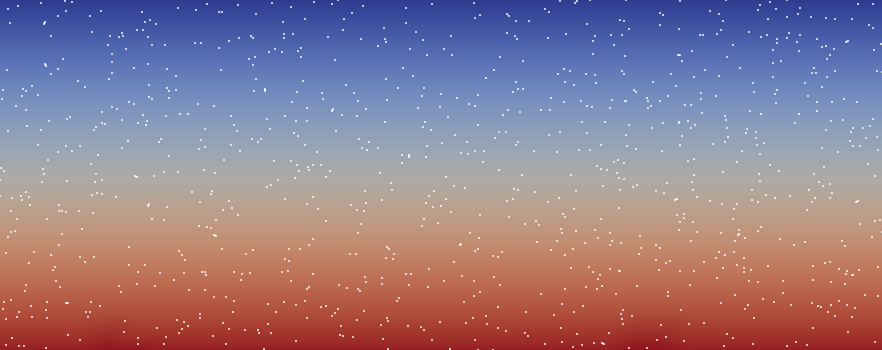
\includegraphics[width=\textwidth]{figures/box_batch0.png}
        \caption{Caption}
        \label{fig:my_label}
    \end{subfigure}
    \hfill
    \begin{subfigure}{0.49\textwidth}
        \centering
        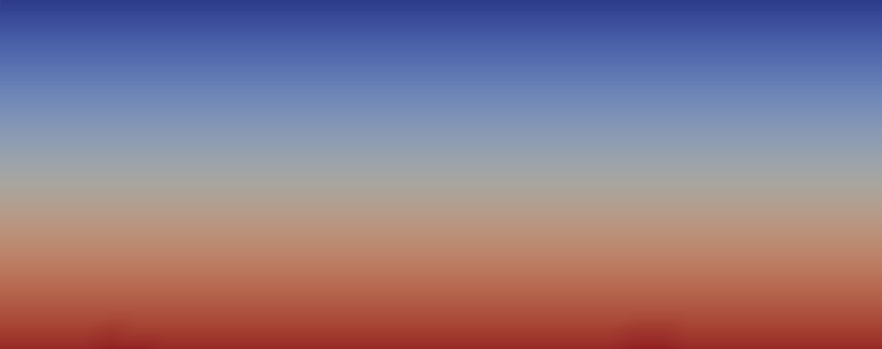
\includegraphics[width=\textwidth]{figures/box_2pp0.png}
        \caption{Caption}
        \label{fig:my_label}
    \end{subfigure}
    %
    \begin{subfigure}{0.49\textwidth}
        \centering
        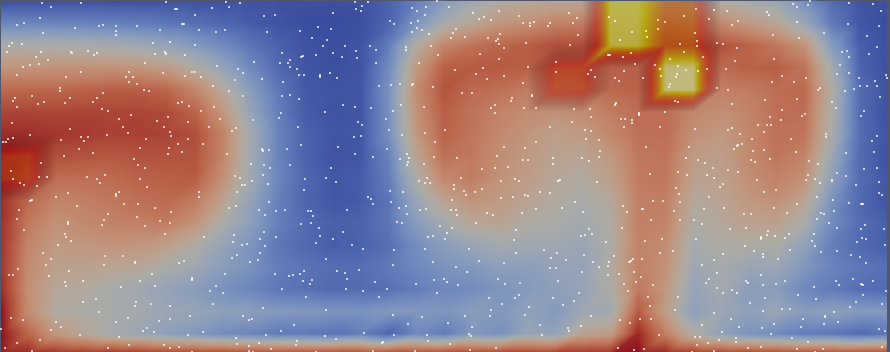
\includegraphics[width=\textwidth]{figures/box_batch38.png}
        \caption{Caption}
        \label{fig:my_label}
    \end{subfigure}
    \hfill
    \begin{subfigure}{0.49\textwidth}
        \centering
        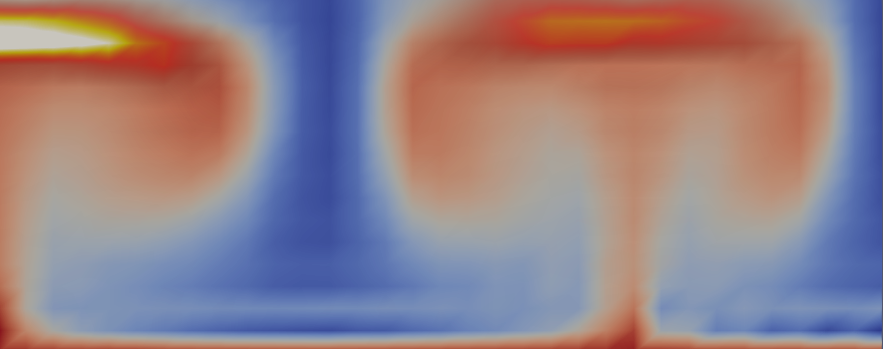
\includegraphics[width=\textwidth]{figures/box_2pp38.png}
        \caption{Caption}
        \label{fig:my_label}
    \end{subfigure}
    %
    \begin{subfigure}{0.49\textwidth}
        \centering
        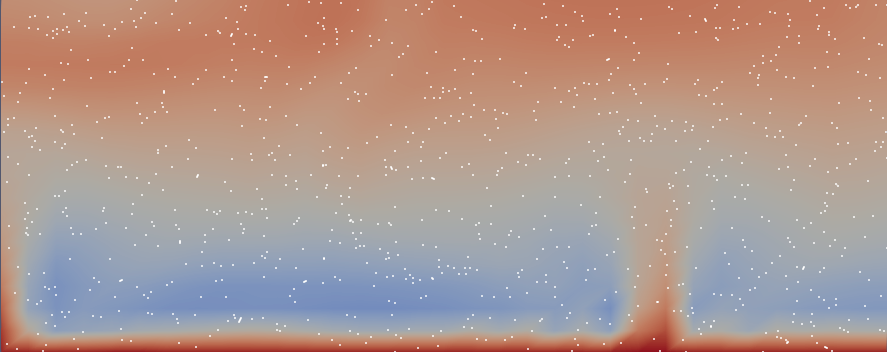
\includegraphics[width=\textwidth]{figures/box_batch79.png}
        \caption{Caption}
        \label{fig:my_label}
    \end{subfigure}
    \hfill
    \begin{subfigure}{0.49\textwidth}
        \centering
        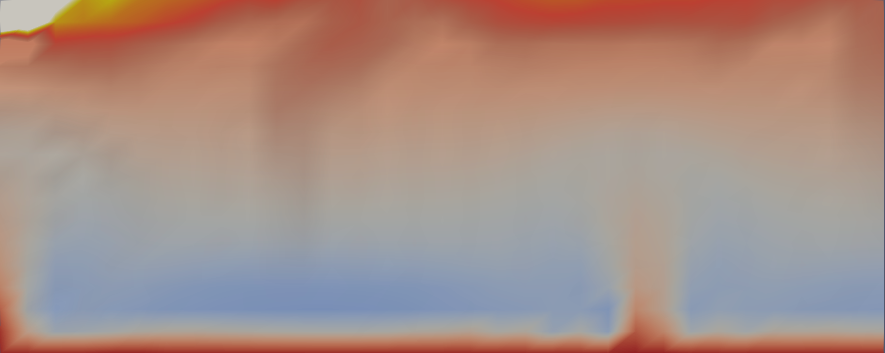
\includegraphics[width=\textwidth]{figures/box_2pp77.png}
        \caption{Caption}
        \label{fig:my_label}
    \end{subfigure}
\end{figure}

\subsection{Performance}

\begin{figure}
    \centering
    \begin{subfigure}{0.49\columnwidth}
        \centering
        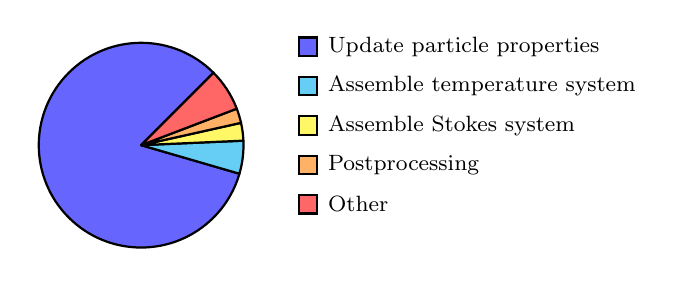
\begin{tikzpicture}
            \pie[hide number, radius=1.3, rotate=45, text=legend] {
                83/ \footnotesize{Update particle properties},
                5.2/ \footnotesize{Assemble temperature system},
                2.8/ \footnotesize{Assemble Stokes system},
                2.3/ \footnotesize{Postprocessing},
                6.7/ \footnotesize{Other}
            }
        \end{tikzpicture}
        \caption{A breakdown of the runtime for the particle property plugin.}
        \label{fig:perf_batch_pie}
    \end{subfigure}
    \hfill
    \begin{subfigure}{0.49\columnwidth}
        \centering
        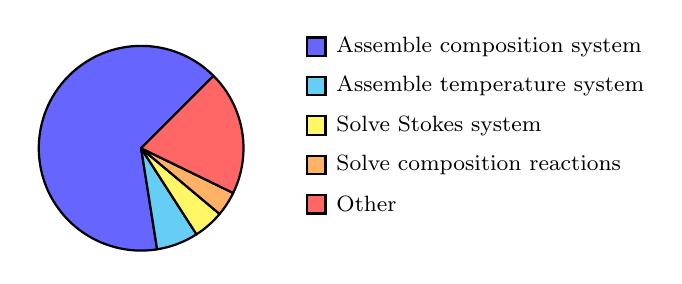
\begin{tikzpicture}
            \pie[hide number, radius=1.3, rotate=45, text=legend] {
                65/ \footnotesize{Assemble composition system},
                6.6/ \footnotesize{Assemble temperature system},
                4.8/ \footnotesize{Solve Stokes system},
                3.9/ \footnotesize{Solve composition reactions},
                19.7/ \footnotesize{Other}
            }
        \end{tikzpicture}
        \caption{A breakdown of the runtime for the material model plugin.}
        \label{fig:perf_2pp_pie}
    \end{subfigure}
    %
    \caption{
        A comparison of the breakdown of runtime spent in the different elements of ASPECT between the particle property and material model approaches to tracking the composition.
        In both cases the \texttt{simple.dat} data set for Perple\_X has been used and the analysis has been drawn from the closed box experiments.
        The actual runtime comparison between the two approaches is discussed in Section~\ref{sec:???}.
    }
    \label{fig:perf_pie}
\end{figure}

\subsubsection{Load balancing}

\begin{figure}
    \centering
    %% Creator: Matplotlib, PGF backend
%%
%% To include the figure in your LaTeX document, write
%%   \input{<filename>.pgf}
%%
%% Make sure the required packages are loaded in your preamble
%%   \usepackage{pgf}
%%
%% Figures using additional raster images can only be included by \input if
%% they are in the same directory as the main LaTeX file. For loading figures
%% from other directories you can use the `import` package
%%   \usepackage{import}
%% and then include the figures with
%%   \import{<path to file>}{<filename>.pgf}
%%
%% Matplotlib used the following preamble
%%   \usepackage{fontspec}
%%   \setmainfont{DejaVuSerif.ttf}[Path=/home/connor/.local/lib/python3.8/site-packages/matplotlib/mpl-data/fonts/ttf/]
%%   \setsansfont{DejaVuSans.ttf}[Path=/home/connor/.local/lib/python3.8/site-packages/matplotlib/mpl-data/fonts/ttf/]
%%   \setmonofont{DejaVuSansMono.ttf}[Path=/home/connor/.local/lib/python3.8/site-packages/matplotlib/mpl-data/fonts/ttf/]
%%
\begingroup%
\makeatletter%
\begin{pgfpicture}%
\pgfpathrectangle{\pgfpointorigin}{\pgfqpoint{3.955386in}{3.018785in}}%
\pgfusepath{use as bounding box, clip}%
\begin{pgfscope}%
\pgfsetbuttcap%
\pgfsetmiterjoin%
\definecolor{currentfill}{rgb}{1.000000,1.000000,1.000000}%
\pgfsetfillcolor{currentfill}%
\pgfsetlinewidth{0.000000pt}%
\definecolor{currentstroke}{rgb}{1.000000,1.000000,1.000000}%
\pgfsetstrokecolor{currentstroke}%
\pgfsetdash{}{0pt}%
\pgfpathmoveto{\pgfqpoint{-0.000000in}{0.000000in}}%
\pgfpathlineto{\pgfqpoint{3.955386in}{0.000000in}}%
\pgfpathlineto{\pgfqpoint{3.955386in}{3.018785in}}%
\pgfpathlineto{\pgfqpoint{-0.000000in}{3.018785in}}%
\pgfpathclose%
\pgfusepath{fill}%
\end{pgfscope}%
\begin{pgfscope}%
\pgfsetbuttcap%
\pgfsetmiterjoin%
\definecolor{currentfill}{rgb}{1.000000,1.000000,1.000000}%
\pgfsetfillcolor{currentfill}%
\pgfsetlinewidth{0.000000pt}%
\definecolor{currentstroke}{rgb}{0.000000,0.000000,0.000000}%
\pgfsetstrokecolor{currentstroke}%
\pgfsetstrokeopacity{0.000000}%
\pgfsetdash{}{0pt}%
\pgfpathmoveto{\pgfqpoint{0.511159in}{0.469412in}}%
\pgfpathlineto{\pgfqpoint{3.798197in}{0.469412in}}%
\pgfpathlineto{\pgfqpoint{3.798197in}{2.918785in}}%
\pgfpathlineto{\pgfqpoint{0.511159in}{2.918785in}}%
\pgfpathclose%
\pgfusepath{fill}%
\end{pgfscope}%
\begin{pgfscope}%
\pgfsetbuttcap%
\pgfsetroundjoin%
\definecolor{currentfill}{rgb}{0.000000,0.000000,0.000000}%
\pgfsetfillcolor{currentfill}%
\pgfsetlinewidth{0.803000pt}%
\definecolor{currentstroke}{rgb}{0.000000,0.000000,0.000000}%
\pgfsetstrokecolor{currentstroke}%
\pgfsetdash{}{0pt}%
\pgfsys@defobject{currentmarker}{\pgfqpoint{0.000000in}{-0.048611in}}{\pgfqpoint{0.000000in}{0.000000in}}{%
\pgfpathmoveto{\pgfqpoint{0.000000in}{0.000000in}}%
\pgfpathlineto{\pgfqpoint{0.000000in}{-0.048611in}}%
\pgfusepath{stroke,fill}%
}%
\begin{pgfscope}%
\pgfsys@transformshift{0.660570in}{0.469412in}%
\pgfsys@useobject{currentmarker}{}%
\end{pgfscope}%
\end{pgfscope}%
\begin{pgfscope}%
\definecolor{textcolor}{rgb}{0.000000,0.000000,0.000000}%
\pgfsetstrokecolor{textcolor}%
\pgfsetfillcolor{textcolor}%
\pgftext[x=0.660570in,y=0.372189in,,top]{\color{textcolor}\rmfamily\fontsize{8.000000}{9.600000}\selectfont \(\displaystyle 0\)}%
\end{pgfscope}%
\begin{pgfscope}%
\pgfsetbuttcap%
\pgfsetroundjoin%
\definecolor{currentfill}{rgb}{0.000000,0.000000,0.000000}%
\pgfsetfillcolor{currentfill}%
\pgfsetlinewidth{0.803000pt}%
\definecolor{currentstroke}{rgb}{0.000000,0.000000,0.000000}%
\pgfsetstrokecolor{currentstroke}%
\pgfsetdash{}{0pt}%
\pgfsys@defobject{currentmarker}{\pgfqpoint{0.000000in}{-0.048611in}}{\pgfqpoint{0.000000in}{0.000000in}}{%
\pgfpathmoveto{\pgfqpoint{0.000000in}{0.000000in}}%
\pgfpathlineto{\pgfqpoint{0.000000in}{-0.048611in}}%
\pgfusepath{stroke,fill}%
}%
\begin{pgfscope}%
\pgfsys@transformshift{1.158606in}{0.469412in}%
\pgfsys@useobject{currentmarker}{}%
\end{pgfscope}%
\end{pgfscope}%
\begin{pgfscope}%
\definecolor{textcolor}{rgb}{0.000000,0.000000,0.000000}%
\pgfsetstrokecolor{textcolor}%
\pgfsetfillcolor{textcolor}%
\pgftext[x=1.158606in,y=0.372189in,,top]{\color{textcolor}\rmfamily\fontsize{8.000000}{9.600000}\selectfont \(\displaystyle 500000\)}%
\end{pgfscope}%
\begin{pgfscope}%
\pgfsetbuttcap%
\pgfsetroundjoin%
\definecolor{currentfill}{rgb}{0.000000,0.000000,0.000000}%
\pgfsetfillcolor{currentfill}%
\pgfsetlinewidth{0.803000pt}%
\definecolor{currentstroke}{rgb}{0.000000,0.000000,0.000000}%
\pgfsetstrokecolor{currentstroke}%
\pgfsetdash{}{0pt}%
\pgfsys@defobject{currentmarker}{\pgfqpoint{0.000000in}{-0.048611in}}{\pgfqpoint{0.000000in}{0.000000in}}{%
\pgfpathmoveto{\pgfqpoint{0.000000in}{0.000000in}}%
\pgfpathlineto{\pgfqpoint{0.000000in}{-0.048611in}}%
\pgfusepath{stroke,fill}%
}%
\begin{pgfscope}%
\pgfsys@transformshift{1.656642in}{0.469412in}%
\pgfsys@useobject{currentmarker}{}%
\end{pgfscope}%
\end{pgfscope}%
\begin{pgfscope}%
\definecolor{textcolor}{rgb}{0.000000,0.000000,0.000000}%
\pgfsetstrokecolor{textcolor}%
\pgfsetfillcolor{textcolor}%
\pgftext[x=1.656642in,y=0.372189in,,top]{\color{textcolor}\rmfamily\fontsize{8.000000}{9.600000}\selectfont \(\displaystyle 1000000\)}%
\end{pgfscope}%
\begin{pgfscope}%
\pgfsetbuttcap%
\pgfsetroundjoin%
\definecolor{currentfill}{rgb}{0.000000,0.000000,0.000000}%
\pgfsetfillcolor{currentfill}%
\pgfsetlinewidth{0.803000pt}%
\definecolor{currentstroke}{rgb}{0.000000,0.000000,0.000000}%
\pgfsetstrokecolor{currentstroke}%
\pgfsetdash{}{0pt}%
\pgfsys@defobject{currentmarker}{\pgfqpoint{0.000000in}{-0.048611in}}{\pgfqpoint{0.000000in}{0.000000in}}{%
\pgfpathmoveto{\pgfqpoint{0.000000in}{0.000000in}}%
\pgfpathlineto{\pgfqpoint{0.000000in}{-0.048611in}}%
\pgfusepath{stroke,fill}%
}%
\begin{pgfscope}%
\pgfsys@transformshift{2.154678in}{0.469412in}%
\pgfsys@useobject{currentmarker}{}%
\end{pgfscope}%
\end{pgfscope}%
\begin{pgfscope}%
\definecolor{textcolor}{rgb}{0.000000,0.000000,0.000000}%
\pgfsetstrokecolor{textcolor}%
\pgfsetfillcolor{textcolor}%
\pgftext[x=2.154678in,y=0.372189in,,top]{\color{textcolor}\rmfamily\fontsize{8.000000}{9.600000}\selectfont \(\displaystyle 1500000\)}%
\end{pgfscope}%
\begin{pgfscope}%
\pgfsetbuttcap%
\pgfsetroundjoin%
\definecolor{currentfill}{rgb}{0.000000,0.000000,0.000000}%
\pgfsetfillcolor{currentfill}%
\pgfsetlinewidth{0.803000pt}%
\definecolor{currentstroke}{rgb}{0.000000,0.000000,0.000000}%
\pgfsetstrokecolor{currentstroke}%
\pgfsetdash{}{0pt}%
\pgfsys@defobject{currentmarker}{\pgfqpoint{0.000000in}{-0.048611in}}{\pgfqpoint{0.000000in}{0.000000in}}{%
\pgfpathmoveto{\pgfqpoint{0.000000in}{0.000000in}}%
\pgfpathlineto{\pgfqpoint{0.000000in}{-0.048611in}}%
\pgfusepath{stroke,fill}%
}%
\begin{pgfscope}%
\pgfsys@transformshift{2.652714in}{0.469412in}%
\pgfsys@useobject{currentmarker}{}%
\end{pgfscope}%
\end{pgfscope}%
\begin{pgfscope}%
\definecolor{textcolor}{rgb}{0.000000,0.000000,0.000000}%
\pgfsetstrokecolor{textcolor}%
\pgfsetfillcolor{textcolor}%
\pgftext[x=2.652714in,y=0.372189in,,top]{\color{textcolor}\rmfamily\fontsize{8.000000}{9.600000}\selectfont \(\displaystyle 2000000\)}%
\end{pgfscope}%
\begin{pgfscope}%
\pgfsetbuttcap%
\pgfsetroundjoin%
\definecolor{currentfill}{rgb}{0.000000,0.000000,0.000000}%
\pgfsetfillcolor{currentfill}%
\pgfsetlinewidth{0.803000pt}%
\definecolor{currentstroke}{rgb}{0.000000,0.000000,0.000000}%
\pgfsetstrokecolor{currentstroke}%
\pgfsetdash{}{0pt}%
\pgfsys@defobject{currentmarker}{\pgfqpoint{0.000000in}{-0.048611in}}{\pgfqpoint{0.000000in}{0.000000in}}{%
\pgfpathmoveto{\pgfqpoint{0.000000in}{0.000000in}}%
\pgfpathlineto{\pgfqpoint{0.000000in}{-0.048611in}}%
\pgfusepath{stroke,fill}%
}%
\begin{pgfscope}%
\pgfsys@transformshift{3.150750in}{0.469412in}%
\pgfsys@useobject{currentmarker}{}%
\end{pgfscope}%
\end{pgfscope}%
\begin{pgfscope}%
\definecolor{textcolor}{rgb}{0.000000,0.000000,0.000000}%
\pgfsetstrokecolor{textcolor}%
\pgfsetfillcolor{textcolor}%
\pgftext[x=3.150750in,y=0.372189in,,top]{\color{textcolor}\rmfamily\fontsize{8.000000}{9.600000}\selectfont \(\displaystyle 2500000\)}%
\end{pgfscope}%
\begin{pgfscope}%
\pgfsetbuttcap%
\pgfsetroundjoin%
\definecolor{currentfill}{rgb}{0.000000,0.000000,0.000000}%
\pgfsetfillcolor{currentfill}%
\pgfsetlinewidth{0.803000pt}%
\definecolor{currentstroke}{rgb}{0.000000,0.000000,0.000000}%
\pgfsetstrokecolor{currentstroke}%
\pgfsetdash{}{0pt}%
\pgfsys@defobject{currentmarker}{\pgfqpoint{0.000000in}{-0.048611in}}{\pgfqpoint{0.000000in}{0.000000in}}{%
\pgfpathmoveto{\pgfqpoint{0.000000in}{0.000000in}}%
\pgfpathlineto{\pgfqpoint{0.000000in}{-0.048611in}}%
\pgfusepath{stroke,fill}%
}%
\begin{pgfscope}%
\pgfsys@transformshift{3.648786in}{0.469412in}%
\pgfsys@useobject{currentmarker}{}%
\end{pgfscope}%
\end{pgfscope}%
\begin{pgfscope}%
\definecolor{textcolor}{rgb}{0.000000,0.000000,0.000000}%
\pgfsetstrokecolor{textcolor}%
\pgfsetfillcolor{textcolor}%
\pgftext[x=3.648786in,y=0.372189in,,top]{\color{textcolor}\rmfamily\fontsize{8.000000}{9.600000}\selectfont \(\displaystyle 3000000\)}%
\end{pgfscope}%
\begin{pgfscope}%
\definecolor{textcolor}{rgb}{0.000000,0.000000,0.000000}%
\pgfsetstrokecolor{textcolor}%
\pgfsetfillcolor{textcolor}%
\pgftext[x=2.154678in,y=0.209104in,,top]{\color{textcolor}\rmfamily\fontsize{8.000000}{9.600000}\selectfont Time (years)}%
\end{pgfscope}%
\begin{pgfscope}%
\pgfsetbuttcap%
\pgfsetroundjoin%
\definecolor{currentfill}{rgb}{0.000000,0.000000,0.000000}%
\pgfsetfillcolor{currentfill}%
\pgfsetlinewidth{0.803000pt}%
\definecolor{currentstroke}{rgb}{0.000000,0.000000,0.000000}%
\pgfsetstrokecolor{currentstroke}%
\pgfsetdash{}{0pt}%
\pgfsys@defobject{currentmarker}{\pgfqpoint{-0.048611in}{0.000000in}}{\pgfqpoint{0.000000in}{0.000000in}}{%
\pgfpathmoveto{\pgfqpoint{0.000000in}{0.000000in}}%
\pgfpathlineto{\pgfqpoint{-0.048611in}{0.000000in}}%
\pgfusepath{stroke,fill}%
}%
\begin{pgfscope}%
\pgfsys@transformshift{0.511159in}{0.594366in}%
\pgfsys@useobject{currentmarker}{}%
\end{pgfscope}%
\end{pgfscope}%
\begin{pgfscope}%
\definecolor{textcolor}{rgb}{0.000000,0.000000,0.000000}%
\pgfsetstrokecolor{textcolor}%
\pgfsetfillcolor{textcolor}%
\pgftext[x=0.263086in,y=0.552156in,left,base]{\color{textcolor}\rmfamily\fontsize{8.000000}{9.600000}\selectfont \(\displaystyle 0.1\)}%
\end{pgfscope}%
\begin{pgfscope}%
\pgfsetbuttcap%
\pgfsetroundjoin%
\definecolor{currentfill}{rgb}{0.000000,0.000000,0.000000}%
\pgfsetfillcolor{currentfill}%
\pgfsetlinewidth{0.803000pt}%
\definecolor{currentstroke}{rgb}{0.000000,0.000000,0.000000}%
\pgfsetstrokecolor{currentstroke}%
\pgfsetdash{}{0pt}%
\pgfsys@defobject{currentmarker}{\pgfqpoint{-0.048611in}{0.000000in}}{\pgfqpoint{0.000000in}{0.000000in}}{%
\pgfpathmoveto{\pgfqpoint{0.000000in}{0.000000in}}%
\pgfpathlineto{\pgfqpoint{-0.048611in}{0.000000in}}%
\pgfusepath{stroke,fill}%
}%
\begin{pgfscope}%
\pgfsys@transformshift{0.511159in}{0.934838in}%
\pgfsys@useobject{currentmarker}{}%
\end{pgfscope}%
\end{pgfscope}%
\begin{pgfscope}%
\definecolor{textcolor}{rgb}{0.000000,0.000000,0.000000}%
\pgfsetstrokecolor{textcolor}%
\pgfsetfillcolor{textcolor}%
\pgftext[x=0.263086in,y=0.892628in,left,base]{\color{textcolor}\rmfamily\fontsize{8.000000}{9.600000}\selectfont \(\displaystyle 0.2\)}%
\end{pgfscope}%
\begin{pgfscope}%
\pgfsetbuttcap%
\pgfsetroundjoin%
\definecolor{currentfill}{rgb}{0.000000,0.000000,0.000000}%
\pgfsetfillcolor{currentfill}%
\pgfsetlinewidth{0.803000pt}%
\definecolor{currentstroke}{rgb}{0.000000,0.000000,0.000000}%
\pgfsetstrokecolor{currentstroke}%
\pgfsetdash{}{0pt}%
\pgfsys@defobject{currentmarker}{\pgfqpoint{-0.048611in}{0.000000in}}{\pgfqpoint{0.000000in}{0.000000in}}{%
\pgfpathmoveto{\pgfqpoint{0.000000in}{0.000000in}}%
\pgfpathlineto{\pgfqpoint{-0.048611in}{0.000000in}}%
\pgfusepath{stroke,fill}%
}%
\begin{pgfscope}%
\pgfsys@transformshift{0.511159in}{1.275310in}%
\pgfsys@useobject{currentmarker}{}%
\end{pgfscope}%
\end{pgfscope}%
\begin{pgfscope}%
\definecolor{textcolor}{rgb}{0.000000,0.000000,0.000000}%
\pgfsetstrokecolor{textcolor}%
\pgfsetfillcolor{textcolor}%
\pgftext[x=0.263086in,y=1.233100in,left,base]{\color{textcolor}\rmfamily\fontsize{8.000000}{9.600000}\selectfont \(\displaystyle 0.3\)}%
\end{pgfscope}%
\begin{pgfscope}%
\pgfsetbuttcap%
\pgfsetroundjoin%
\definecolor{currentfill}{rgb}{0.000000,0.000000,0.000000}%
\pgfsetfillcolor{currentfill}%
\pgfsetlinewidth{0.803000pt}%
\definecolor{currentstroke}{rgb}{0.000000,0.000000,0.000000}%
\pgfsetstrokecolor{currentstroke}%
\pgfsetdash{}{0pt}%
\pgfsys@defobject{currentmarker}{\pgfqpoint{-0.048611in}{0.000000in}}{\pgfqpoint{0.000000in}{0.000000in}}{%
\pgfpathmoveto{\pgfqpoint{0.000000in}{0.000000in}}%
\pgfpathlineto{\pgfqpoint{-0.048611in}{0.000000in}}%
\pgfusepath{stroke,fill}%
}%
\begin{pgfscope}%
\pgfsys@transformshift{0.511159in}{1.615782in}%
\pgfsys@useobject{currentmarker}{}%
\end{pgfscope}%
\end{pgfscope}%
\begin{pgfscope}%
\definecolor{textcolor}{rgb}{0.000000,0.000000,0.000000}%
\pgfsetstrokecolor{textcolor}%
\pgfsetfillcolor{textcolor}%
\pgftext[x=0.263086in,y=1.573572in,left,base]{\color{textcolor}\rmfamily\fontsize{8.000000}{9.600000}\selectfont \(\displaystyle 0.4\)}%
\end{pgfscope}%
\begin{pgfscope}%
\pgfsetbuttcap%
\pgfsetroundjoin%
\definecolor{currentfill}{rgb}{0.000000,0.000000,0.000000}%
\pgfsetfillcolor{currentfill}%
\pgfsetlinewidth{0.803000pt}%
\definecolor{currentstroke}{rgb}{0.000000,0.000000,0.000000}%
\pgfsetstrokecolor{currentstroke}%
\pgfsetdash{}{0pt}%
\pgfsys@defobject{currentmarker}{\pgfqpoint{-0.048611in}{0.000000in}}{\pgfqpoint{0.000000in}{0.000000in}}{%
\pgfpathmoveto{\pgfqpoint{0.000000in}{0.000000in}}%
\pgfpathlineto{\pgfqpoint{-0.048611in}{0.000000in}}%
\pgfusepath{stroke,fill}%
}%
\begin{pgfscope}%
\pgfsys@transformshift{0.511159in}{1.956254in}%
\pgfsys@useobject{currentmarker}{}%
\end{pgfscope}%
\end{pgfscope}%
\begin{pgfscope}%
\definecolor{textcolor}{rgb}{0.000000,0.000000,0.000000}%
\pgfsetstrokecolor{textcolor}%
\pgfsetfillcolor{textcolor}%
\pgftext[x=0.263086in,y=1.914044in,left,base]{\color{textcolor}\rmfamily\fontsize{8.000000}{9.600000}\selectfont \(\displaystyle 0.5\)}%
\end{pgfscope}%
\begin{pgfscope}%
\pgfsetbuttcap%
\pgfsetroundjoin%
\definecolor{currentfill}{rgb}{0.000000,0.000000,0.000000}%
\pgfsetfillcolor{currentfill}%
\pgfsetlinewidth{0.803000pt}%
\definecolor{currentstroke}{rgb}{0.000000,0.000000,0.000000}%
\pgfsetstrokecolor{currentstroke}%
\pgfsetdash{}{0pt}%
\pgfsys@defobject{currentmarker}{\pgfqpoint{-0.048611in}{0.000000in}}{\pgfqpoint{0.000000in}{0.000000in}}{%
\pgfpathmoveto{\pgfqpoint{0.000000in}{0.000000in}}%
\pgfpathlineto{\pgfqpoint{-0.048611in}{0.000000in}}%
\pgfusepath{stroke,fill}%
}%
\begin{pgfscope}%
\pgfsys@transformshift{0.511159in}{2.296726in}%
\pgfsys@useobject{currentmarker}{}%
\end{pgfscope}%
\end{pgfscope}%
\begin{pgfscope}%
\definecolor{textcolor}{rgb}{0.000000,0.000000,0.000000}%
\pgfsetstrokecolor{textcolor}%
\pgfsetfillcolor{textcolor}%
\pgftext[x=0.263086in,y=2.254516in,left,base]{\color{textcolor}\rmfamily\fontsize{8.000000}{9.600000}\selectfont \(\displaystyle 0.6\)}%
\end{pgfscope}%
\begin{pgfscope}%
\pgfsetbuttcap%
\pgfsetroundjoin%
\definecolor{currentfill}{rgb}{0.000000,0.000000,0.000000}%
\pgfsetfillcolor{currentfill}%
\pgfsetlinewidth{0.803000pt}%
\definecolor{currentstroke}{rgb}{0.000000,0.000000,0.000000}%
\pgfsetstrokecolor{currentstroke}%
\pgfsetdash{}{0pt}%
\pgfsys@defobject{currentmarker}{\pgfqpoint{-0.048611in}{0.000000in}}{\pgfqpoint{0.000000in}{0.000000in}}{%
\pgfpathmoveto{\pgfqpoint{0.000000in}{0.000000in}}%
\pgfpathlineto{\pgfqpoint{-0.048611in}{0.000000in}}%
\pgfusepath{stroke,fill}%
}%
\begin{pgfscope}%
\pgfsys@transformshift{0.511159in}{2.637198in}%
\pgfsys@useobject{currentmarker}{}%
\end{pgfscope}%
\end{pgfscope}%
\begin{pgfscope}%
\definecolor{textcolor}{rgb}{0.000000,0.000000,0.000000}%
\pgfsetstrokecolor{textcolor}%
\pgfsetfillcolor{textcolor}%
\pgftext[x=0.263086in,y=2.594988in,left,base]{\color{textcolor}\rmfamily\fontsize{8.000000}{9.600000}\selectfont \(\displaystyle 0.7\)}%
\end{pgfscope}%
\begin{pgfscope}%
\definecolor{textcolor}{rgb}{0.000000,0.000000,0.000000}%
\pgfsetstrokecolor{textcolor}%
\pgfsetfillcolor{textcolor}%
\pgftext[x=0.207530in,y=1.694098in,,bottom,rotate=90.000000]{\color{textcolor}\rmfamily\fontsize{8.000000}{9.600000}\selectfont ???}%
\end{pgfscope}%
\begin{pgfscope}%
\pgfpathrectangle{\pgfqpoint{0.511159in}{0.469412in}}{\pgfqpoint{3.287038in}{2.449373in}}%
\pgfusepath{clip}%
\pgfsetrectcap%
\pgfsetroundjoin%
\pgfsetlinewidth{1.505625pt}%
\definecolor{currentstroke}{rgb}{0.121569,0.466667,0.705882}%
\pgfsetstrokecolor{currentstroke}%
\pgfsetdash{}{0pt}%
\pgfpathmoveto{\pgfqpoint{0.660570in}{0.580747in}}%
\pgfpathlineto{\pgfqpoint{0.760177in}{0.662460in}}%
\pgfpathlineto{\pgfqpoint{0.859784in}{0.662460in}}%
\pgfpathlineto{\pgfqpoint{1.058999in}{0.744173in}}%
\pgfpathlineto{\pgfqpoint{1.158606in}{0.907600in}}%
\pgfpathlineto{\pgfqpoint{1.258213in}{0.907600in}}%
\pgfpathlineto{\pgfqpoint{1.339843in}{1.030170in}}%
\pgfpathlineto{\pgfqpoint{1.380510in}{0.907600in}}%
\pgfpathlineto{\pgfqpoint{1.408154in}{0.866743in}}%
\pgfpathlineto{\pgfqpoint{1.429141in}{0.785030in}}%
\pgfpathlineto{\pgfqpoint{1.446071in}{0.785030in}}%
\pgfpathlineto{\pgfqpoint{1.460304in}{0.866743in}}%
\pgfpathlineto{\pgfqpoint{1.483459in}{0.866743in}}%
\pgfpathlineto{\pgfqpoint{1.493104in}{0.948457in}}%
\pgfpathlineto{\pgfqpoint{1.501837in}{0.948457in}}%
\pgfpathlineto{\pgfqpoint{1.509850in}{1.030170in}}%
\pgfpathlineto{\pgfqpoint{1.524239in}{0.948457in}}%
\pgfpathlineto{\pgfqpoint{1.530789in}{1.111883in}}%
\pgfpathlineto{\pgfqpoint{1.537004in}{1.193597in}}%
\pgfpathlineto{\pgfqpoint{1.542939in}{1.071027in}}%
\pgfpathlineto{\pgfqpoint{1.548638in}{1.193597in}}%
\pgfpathlineto{\pgfqpoint{1.554138in}{1.111883in}}%
\pgfpathlineto{\pgfqpoint{1.564663in}{1.030170in}}%
\pgfpathlineto{\pgfqpoint{1.569738in}{0.825887in}}%
\pgfpathlineto{\pgfqpoint{1.574713in}{0.825887in}}%
\pgfpathlineto{\pgfqpoint{1.579608in}{0.907600in}}%
\pgfpathlineto{\pgfqpoint{1.584436in}{1.234453in}}%
\pgfpathlineto{\pgfqpoint{1.589210in}{1.275310in}}%
\pgfpathlineto{\pgfqpoint{1.593942in}{1.193597in}}%
\pgfpathlineto{\pgfqpoint{1.598644in}{1.397880in}}%
\pgfpathlineto{\pgfqpoint{1.603327in}{1.111883in}}%
\pgfpathlineto{\pgfqpoint{1.612680in}{1.275310in}}%
\pgfpathlineto{\pgfqpoint{1.617369in}{1.071027in}}%
\pgfpathlineto{\pgfqpoint{1.626820in}{1.071027in}}%
\pgfpathlineto{\pgfqpoint{1.631601in}{1.152740in}}%
\pgfpathlineto{\pgfqpoint{1.636430in}{1.275310in}}%
\pgfpathlineto{\pgfqpoint{1.641316in}{1.316167in}}%
\pgfpathlineto{\pgfqpoint{1.646269in}{1.397880in}}%
\pgfpathlineto{\pgfqpoint{1.651298in}{1.438737in}}%
\pgfpathlineto{\pgfqpoint{1.656412in}{1.561307in}}%
\pgfpathlineto{\pgfqpoint{1.661620in}{1.397880in}}%
\pgfpathlineto{\pgfqpoint{1.666933in}{1.152740in}}%
\pgfpathlineto{\pgfqpoint{1.672360in}{1.193597in}}%
\pgfpathlineto{\pgfqpoint{1.677911in}{1.152740in}}%
\pgfpathlineto{\pgfqpoint{1.683598in}{1.316167in}}%
\pgfpathlineto{\pgfqpoint{1.689432in}{1.193597in}}%
\pgfpathlineto{\pgfqpoint{1.701589in}{1.193597in}}%
\pgfpathlineto{\pgfqpoint{1.707676in}{1.397880in}}%
\pgfpathlineto{\pgfqpoint{1.713635in}{1.438737in}}%
\pgfpathlineto{\pgfqpoint{1.719511in}{1.602163in}}%
\pgfpathlineto{\pgfqpoint{1.731190in}{1.520450in}}%
\pgfpathlineto{\pgfqpoint{1.737067in}{1.397880in}}%
\pgfpathlineto{\pgfqpoint{1.743012in}{1.397880in}}%
\pgfpathlineto{\pgfqpoint{1.749055in}{1.357023in}}%
\pgfpathlineto{\pgfqpoint{1.755207in}{1.152740in}}%
\pgfpathlineto{\pgfqpoint{1.761487in}{1.234453in}}%
\pgfpathlineto{\pgfqpoint{1.767919in}{1.275310in}}%
\pgfpathlineto{\pgfqpoint{1.774524in}{1.152740in}}%
\pgfpathlineto{\pgfqpoint{1.781322in}{1.152740in}}%
\pgfpathlineto{\pgfqpoint{1.795562in}{0.989313in}}%
\pgfpathlineto{\pgfqpoint{1.810752in}{1.071027in}}%
\pgfpathlineto{\pgfqpoint{1.818730in}{1.193597in}}%
\pgfpathlineto{\pgfqpoint{1.826975in}{1.234453in}}%
\pgfpathlineto{\pgfqpoint{1.835493in}{1.234453in}}%
\pgfpathlineto{\pgfqpoint{1.844292in}{1.193597in}}%
\pgfpathlineto{\pgfqpoint{1.853377in}{1.193597in}}%
\pgfpathlineto{\pgfqpoint{1.862751in}{1.152740in}}%
\pgfpathlineto{\pgfqpoint{1.872420in}{1.316167in}}%
\pgfpathlineto{\pgfqpoint{1.882387in}{1.397880in}}%
\pgfpathlineto{\pgfqpoint{1.892656in}{1.397880in}}%
\pgfpathlineto{\pgfqpoint{1.903233in}{1.520450in}}%
\pgfpathlineto{\pgfqpoint{1.914115in}{1.397880in}}%
\pgfpathlineto{\pgfqpoint{1.925299in}{1.438737in}}%
\pgfpathlineto{\pgfqpoint{1.936793in}{1.438737in}}%
\pgfpathlineto{\pgfqpoint{1.948607in}{1.520450in}}%
\pgfpathlineto{\pgfqpoint{1.960750in}{1.724733in}}%
\pgfpathlineto{\pgfqpoint{1.973235in}{1.479593in}}%
\pgfpathlineto{\pgfqpoint{1.986074in}{1.561307in}}%
\pgfpathlineto{\pgfqpoint{1.999283in}{1.520450in}}%
\pgfpathlineto{\pgfqpoint{2.012877in}{1.438737in}}%
\pgfpathlineto{\pgfqpoint{2.026874in}{1.520450in}}%
\pgfpathlineto{\pgfqpoint{2.041290in}{1.438737in}}%
\pgfpathlineto{\pgfqpoint{2.071393in}{1.438737in}}%
\pgfpathlineto{\pgfqpoint{2.087108in}{1.520450in}}%
\pgfpathlineto{\pgfqpoint{2.103289in}{1.561307in}}%
\pgfpathlineto{\pgfqpoint{2.119954in}{1.520450in}}%
\pgfpathlineto{\pgfqpoint{2.137122in}{1.397880in}}%
\pgfpathlineto{\pgfqpoint{2.154813in}{1.397880in}}%
\pgfpathlineto{\pgfqpoint{2.173046in}{1.520450in}}%
\pgfpathlineto{\pgfqpoint{2.191840in}{1.683877in}}%
\pgfpathlineto{\pgfqpoint{2.211215in}{1.724733in}}%
\pgfpathlineto{\pgfqpoint{2.231151in}{1.683877in}}%
\pgfpathlineto{\pgfqpoint{2.251663in}{1.683877in}}%
\pgfpathlineto{\pgfqpoint{2.272769in}{1.602163in}}%
\pgfpathlineto{\pgfqpoint{2.294483in}{1.765590in}}%
\pgfpathlineto{\pgfqpoint{2.316822in}{1.847303in}}%
\pgfpathlineto{\pgfqpoint{2.339803in}{1.888160in}}%
\pgfpathlineto{\pgfqpoint{2.363441in}{1.806447in}}%
\pgfpathlineto{\pgfqpoint{2.387753in}{1.847303in}}%
\pgfpathlineto{\pgfqpoint{2.412754in}{1.806447in}}%
\pgfpathlineto{\pgfqpoint{2.438460in}{1.806447in}}%
\pgfpathlineto{\pgfqpoint{2.464888in}{1.561307in}}%
\pgfpathlineto{\pgfqpoint{2.492054in}{1.561307in}}%
\pgfpathlineto{\pgfqpoint{2.519974in}{1.520450in}}%
\pgfpathlineto{\pgfqpoint{2.548633in}{1.683877in}}%
\pgfpathlineto{\pgfqpoint{2.577998in}{1.765590in}}%
\pgfpathlineto{\pgfqpoint{2.608078in}{1.847303in}}%
\pgfpathlineto{\pgfqpoint{2.638883in}{1.765590in}}%
\pgfpathlineto{\pgfqpoint{2.670422in}{1.643020in}}%
\pgfpathlineto{\pgfqpoint{2.702705in}{1.602163in}}%
\pgfpathlineto{\pgfqpoint{2.735743in}{1.724733in}}%
\pgfpathlineto{\pgfqpoint{2.769548in}{1.806447in}}%
\pgfpathlineto{\pgfqpoint{2.804137in}{1.602163in}}%
\pgfpathlineto{\pgfqpoint{2.839524in}{1.643020in}}%
\pgfpathlineto{\pgfqpoint{2.875698in}{1.683877in}}%
\pgfpathlineto{\pgfqpoint{2.949194in}{1.520450in}}%
\pgfpathlineto{\pgfqpoint{2.986639in}{1.316167in}}%
\pgfpathlineto{\pgfqpoint{3.024666in}{1.397880in}}%
\pgfpathlineto{\pgfqpoint{3.063389in}{1.397880in}}%
\pgfpathlineto{\pgfqpoint{3.102943in}{1.357023in}}%
\pgfpathlineto{\pgfqpoint{3.143447in}{1.152740in}}%
\pgfpathlineto{\pgfqpoint{3.184016in}{1.071027in}}%
\pgfpathlineto{\pgfqpoint{3.223946in}{1.316167in}}%
\pgfpathlineto{\pgfqpoint{3.263378in}{1.357023in}}%
\pgfpathlineto{\pgfqpoint{3.302446in}{1.234453in}}%
\pgfpathlineto{\pgfqpoint{3.341269in}{1.275310in}}%
\pgfpathlineto{\pgfqpoint{3.379951in}{1.152740in}}%
\pgfpathlineto{\pgfqpoint{3.418580in}{1.193597in}}%
\pgfpathlineto{\pgfqpoint{3.495937in}{1.193597in}}%
\pgfpathlineto{\pgfqpoint{3.534758in}{1.152740in}}%
\pgfpathlineto{\pgfqpoint{3.573714in}{1.071027in}}%
\pgfpathlineto{\pgfqpoint{3.612823in}{1.111883in}}%
\pgfpathlineto{\pgfqpoint{3.648786in}{1.152740in}}%
\pgfpathlineto{\pgfqpoint{3.648786in}{1.152740in}}%
\pgfusepath{stroke}%
\end{pgfscope}%
\begin{pgfscope}%
\pgfpathrectangle{\pgfqpoint{0.511159in}{0.469412in}}{\pgfqpoint{3.287038in}{2.449373in}}%
\pgfusepath{clip}%
\pgfsetrectcap%
\pgfsetroundjoin%
\pgfsetlinewidth{1.505625pt}%
\definecolor{currentstroke}{rgb}{1.000000,0.498039,0.054902}%
\pgfsetstrokecolor{currentstroke}%
\pgfsetdash{}{0pt}%
\pgfpathmoveto{\pgfqpoint{0.660570in}{2.807450in}}%
\pgfpathlineto{\pgfqpoint{0.760177in}{2.807450in}}%
\pgfpathlineto{\pgfqpoint{0.859784in}{2.807450in}}%
\pgfpathlineto{\pgfqpoint{0.959391in}{2.807450in}}%
\pgfpathlineto{\pgfqpoint{1.037987in}{2.807450in}}%
\pgfpathlineto{\pgfqpoint{1.068864in}{2.807450in}}%
\pgfpathlineto{\pgfqpoint{1.091797in}{2.807450in}}%
\pgfpathlineto{\pgfqpoint{1.110630in}{2.807450in}}%
\pgfpathlineto{\pgfqpoint{1.126945in}{2.807450in}}%
\pgfpathlineto{\pgfqpoint{1.141593in}{2.807450in}}%
\pgfpathlineto{\pgfqpoint{1.155104in}{2.807450in}}%
\pgfpathlineto{\pgfqpoint{1.167693in}{2.807450in}}%
\pgfpathlineto{\pgfqpoint{1.179602in}{2.807450in}}%
\pgfpathlineto{\pgfqpoint{1.191036in}{2.807450in}}%
\pgfpathlineto{\pgfqpoint{1.202155in}{2.807450in}}%
\pgfpathlineto{\pgfqpoint{1.212628in}{2.807450in}}%
\pgfpathlineto{\pgfqpoint{1.222582in}{2.807450in}}%
\pgfpathlineto{\pgfqpoint{1.232207in}{2.807450in}}%
\pgfpathlineto{\pgfqpoint{1.241649in}{2.807450in}}%
\pgfpathlineto{\pgfqpoint{1.251028in}{2.807450in}}%
\pgfpathlineto{\pgfqpoint{1.260450in}{2.807450in}}%
\pgfpathlineto{\pgfqpoint{1.270005in}{2.807450in}}%
\pgfpathlineto{\pgfqpoint{1.279775in}{2.807450in}}%
\pgfpathlineto{\pgfqpoint{1.289833in}{2.807450in}}%
\pgfpathlineto{\pgfqpoint{1.300244in}{2.807450in}}%
\pgfpathlineto{\pgfqpoint{1.311071in}{2.807450in}}%
\pgfpathlineto{\pgfqpoint{1.322380in}{2.807450in}}%
\pgfpathlineto{\pgfqpoint{1.334238in}{2.807450in}}%
\pgfpathlineto{\pgfqpoint{1.346717in}{2.807450in}}%
\pgfpathlineto{\pgfqpoint{1.359892in}{2.807450in}}%
\pgfpathlineto{\pgfqpoint{1.373846in}{2.807450in}}%
\pgfpathlineto{\pgfqpoint{1.388664in}{2.807450in}}%
\pgfpathlineto{\pgfqpoint{1.404435in}{2.807450in}}%
\pgfpathlineto{\pgfqpoint{1.421242in}{2.807450in}}%
\pgfpathlineto{\pgfqpoint{1.439181in}{2.807450in}}%
\pgfpathlineto{\pgfqpoint{1.458367in}{2.807450in}}%
\pgfpathlineto{\pgfqpoint{1.478498in}{2.807450in}}%
\pgfpathlineto{\pgfqpoint{1.499233in}{2.807450in}}%
\pgfpathlineto{\pgfqpoint{1.521012in}{2.807450in}}%
\pgfpathlineto{\pgfqpoint{1.544381in}{2.807450in}}%
\pgfpathlineto{\pgfqpoint{1.570016in}{2.807450in}}%
\pgfpathlineto{\pgfqpoint{1.598808in}{2.807450in}}%
\pgfpathlineto{\pgfqpoint{1.631494in}{2.807450in}}%
\pgfpathlineto{\pgfqpoint{1.667466in}{2.807450in}}%
\pgfpathlineto{\pgfqpoint{1.707178in}{2.807450in}}%
\pgfpathlineto{\pgfqpoint{1.750568in}{2.807450in}}%
\pgfpathlineto{\pgfqpoint{1.797829in}{2.807450in}}%
\pgfpathlineto{\pgfqpoint{1.848879in}{2.807450in}}%
\pgfpathlineto{\pgfqpoint{1.903129in}{2.807450in}}%
\pgfpathlineto{\pgfqpoint{1.960372in}{2.807450in}}%
\pgfpathlineto{\pgfqpoint{2.020433in}{2.807450in}}%
\pgfpathlineto{\pgfqpoint{2.083273in}{2.807450in}}%
\pgfpathlineto{\pgfqpoint{2.148809in}{2.807450in}}%
\pgfpathlineto{\pgfqpoint{2.216866in}{2.807450in}}%
\pgfpathlineto{\pgfqpoint{2.287239in}{2.807450in}}%
\pgfpathlineto{\pgfqpoint{2.359742in}{2.807450in}}%
\pgfpathlineto{\pgfqpoint{2.434260in}{2.807450in}}%
\pgfpathlineto{\pgfqpoint{2.510722in}{2.807450in}}%
\pgfpathlineto{\pgfqpoint{2.589078in}{2.807450in}}%
\pgfpathlineto{\pgfqpoint{2.669296in}{2.807450in}}%
\pgfpathlineto{\pgfqpoint{2.749722in}{2.807450in}}%
\pgfpathlineto{\pgfqpoint{2.829926in}{2.807450in}}%
\pgfpathlineto{\pgfqpoint{2.910828in}{2.807450in}}%
\pgfpathlineto{\pgfqpoint{2.993422in}{2.807450in}}%
\pgfpathlineto{\pgfqpoint{3.077021in}{2.807450in}}%
\pgfpathlineto{\pgfqpoint{3.156129in}{2.807450in}}%
\pgfpathlineto{\pgfqpoint{3.222452in}{2.807450in}}%
\pgfpathlineto{\pgfqpoint{3.279508in}{2.807450in}}%
\pgfpathlineto{\pgfqpoint{3.355223in}{2.807450in}}%
\pgfpathlineto{\pgfqpoint{3.428243in}{2.807450in}}%
\pgfpathlineto{\pgfqpoint{3.502748in}{2.807450in}}%
\pgfpathlineto{\pgfqpoint{3.528665in}{2.807450in}}%
\pgfpathlineto{\pgfqpoint{3.608684in}{2.807450in}}%
\pgfpathlineto{\pgfqpoint{3.648786in}{2.807450in}}%
\pgfusepath{stroke}%
\end{pgfscope}%
\begin{pgfscope}%
\pgfsetrectcap%
\pgfsetmiterjoin%
\pgfsetlinewidth{0.803000pt}%
\definecolor{currentstroke}{rgb}{0.000000,0.000000,0.000000}%
\pgfsetstrokecolor{currentstroke}%
\pgfsetdash{}{0pt}%
\pgfpathmoveto{\pgfqpoint{0.511159in}{0.469412in}}%
\pgfpathlineto{\pgfqpoint{0.511159in}{2.918785in}}%
\pgfusepath{stroke}%
\end{pgfscope}%
\begin{pgfscope}%
\pgfsetrectcap%
\pgfsetmiterjoin%
\pgfsetlinewidth{0.803000pt}%
\definecolor{currentstroke}{rgb}{0.000000,0.000000,0.000000}%
\pgfsetstrokecolor{currentstroke}%
\pgfsetdash{}{0pt}%
\pgfpathmoveto{\pgfqpoint{3.798197in}{0.469412in}}%
\pgfpathlineto{\pgfqpoint{3.798197in}{2.918785in}}%
\pgfusepath{stroke}%
\end{pgfscope}%
\begin{pgfscope}%
\pgfsetrectcap%
\pgfsetmiterjoin%
\pgfsetlinewidth{0.803000pt}%
\definecolor{currentstroke}{rgb}{0.000000,0.000000,0.000000}%
\pgfsetstrokecolor{currentstroke}%
\pgfsetdash{}{0pt}%
\pgfpathmoveto{\pgfqpoint{0.511159in}{0.469412in}}%
\pgfpathlineto{\pgfqpoint{3.798197in}{0.469412in}}%
\pgfusepath{stroke}%
\end{pgfscope}%
\begin{pgfscope}%
\pgfsetrectcap%
\pgfsetmiterjoin%
\pgfsetlinewidth{0.803000pt}%
\definecolor{currentstroke}{rgb}{0.000000,0.000000,0.000000}%
\pgfsetstrokecolor{currentstroke}%
\pgfsetdash{}{0pt}%
\pgfpathmoveto{\pgfqpoint{0.511159in}{2.918785in}}%
\pgfpathlineto{\pgfqpoint{3.798197in}{2.918785in}}%
\pgfusepath{stroke}%
\end{pgfscope}%
\begin{pgfscope}%
\pgfsetrectcap%
\pgfsetroundjoin%
\pgfsetlinewidth{1.505625pt}%
\definecolor{currentstroke}{rgb}{0.121569,0.466667,0.705882}%
\pgfsetstrokecolor{currentstroke}%
\pgfsetdash{}{0pt}%
\pgfpathmoveto{\pgfqpoint{2.526246in}{0.796072in}}%
\pgfpathlineto{\pgfqpoint{2.748468in}{0.796072in}}%
\pgfusepath{stroke}%
\end{pgfscope}%
\begin{pgfscope}%
\definecolor{textcolor}{rgb}{0.000000,0.000000,0.000000}%
\pgfsetstrokecolor{textcolor}%
\pgfsetfillcolor{textcolor}%
\pgftext[x=2.837357in,y=0.757183in,left,base]{\color{textcolor}\rmfamily\fontsize{8.000000}{9.600000}\selectfont Particle plugin}%
\end{pgfscope}%
\begin{pgfscope}%
\pgfsetrectcap%
\pgfsetroundjoin%
\pgfsetlinewidth{1.505625pt}%
\definecolor{currentstroke}{rgb}{1.000000,0.498039,0.054902}%
\pgfsetstrokecolor{currentstroke}%
\pgfsetdash{}{0pt}%
\pgfpathmoveto{\pgfqpoint{2.526246in}{0.631412in}}%
\pgfpathlineto{\pgfqpoint{2.748468in}{0.631412in}}%
\pgfusepath{stroke}%
\end{pgfscope}%
\begin{pgfscope}%
\definecolor{textcolor}{rgb}{0.000000,0.000000,0.000000}%
\pgfsetstrokecolor{textcolor}%
\pgfsetfillcolor{textcolor}%
\pgftext[x=2.837357in,y=0.592523in,left,base]{\color{textcolor}\rmfamily\fontsize{8.000000}{9.600000}\selectfont Material model}%
\end{pgfscope}%
\end{pgfpicture}%
\makeatother%
\endgroup%

    \caption{Caption}
    \label{fig:load_balancing}
\end{figure}

\section{Discussion}
\label{sec:discussion}
\subsection{Perple\_X data file accuracy}
\label{sec:discussion_perplexdata}

For the Perple\_X problem definition file it was important to use a close approximation of the chemical composition of the upper mantle.
The file initially selected was created by Debaditya Bandyopadhyay and modelled KLB-1 peridotite~\parencite{takahashi_melting_1986} in order to reproduce the results from~\textcite{hollandMeltingPeridotitesGranites2018}.
Unfortunately, the problem file is fairly complex so any single minimisation takes several seconds to complete, posing problems for running many such simulations in ASPECT.
The complexity is due to there being many chemical components used in the file, and these massively increase the number of pseudocompounds used by the linear solving algorithm.
In addition, a further, more critical, problem was encountered when we tried running the material model with this data set.
It turns out that, every time MEEMUM is called, data is added to a static array which slowly fills up\footnote{The array causing the overflow error is called \texttt{sco} and is defined inside of \texttt{perplex\_parameters.h}.}.
The array fills up much faster for the complex KLB-1 data file than for simpler problems and so after a short while the array overflows and the program crashes.

\begin{table}[htb]
    \centering
    \begin{tabular}{c|c|c}
        \textit{Chemical component} & \textit{KLB-1} (\si{\mol}) & \textit{Simplified KLB-1} (\si{\mol}) \\
        \hline
        \ce{K2O} & 0.01 & - \\
        \ce{Na2O} & 0.25 & - \\
        \ce{SiO2} & 38.46 & 38.50 \\ 
        \ce{Al2O3} & 1.77 & - \\
        \ce{CaO} & 2.82 & 2.82 \\
        \ce{MgO} & 50.53 & 50.50 \\
        \ce{FeO} & 5.88 & 5.88 \\
        \ce{TiO2} & 0.07 & - \\
        \ce{Cr2O3} & 0.11 & - \\
        \ce{O2} & 0.05 & -
    \end{tabular}
    \caption{
        Bulk composition of the KLB-1 and simplified KLB-1 data files.
        Only the four most abundant components are used in the latter.
    }
    \label{tab:perplex_models}
\end{table}

No fix could be found for this problem within the time constraints of the project, so we were forced to perform the experiments using a simpler data file, initially intended just for testing (see Table~\ref{tab:perplex_models} for a comparison of bulk compositions of the two).
This simpler file was based upon the KLB-1 data set, so as to remain as consistent as possible with the mantle region of interest, but the composition components with the lowest concentrations, including water, were omitted.
This resulted in a data file that could be solved by MEEMUM in a fraction of the time and was also free from the array overflow error.
Unfortunately, having constructed the file out of a desire for fast performance rather than scientific validity, the results reported above cannot be considered particularly realistic.

To improve the accuracy we present three options: 
(a) use a slightly more accurate data file that still has relatively few pseudocompounds; 
(b) use an advanced data set such as KLB-1 but limit the number of calls to Perple\_X to restrict the rate at which the array fills up; 
or (c) alter either the C++/Fortran interface code or the Perple\_X source directly to avoid the overflow issue entirely.
We propose option (b) as the best solution.
Option (a), while improving the results, will still lead to an inaccurate solution and is fundamentally limited.
Option (c) is highly complex and it is preferable not to alter the original Perple\_X source code (as discussed in Section~\ref{sec:solution_perplexcpp_orig}).
By comparison, option (b) will not affect the validity of the results, assuming that the rate of evaluations is not too coarse, and has the potential to dramatically increase the performance by reducing the number of calls to Perple\_X.

Some specific examples of how this could be achieved are: 
(a) introduce a $p$-$T$ threshold, that may be a function, that only asks to evaluate Perple\_X when there is likely to be melt present; or
(b) add an additional option to the material model so that Perple\_X is evaluated at specified times, for example every \num{10000} years.
Option (b) mirrors the approach taken by the particle property plugin although such an approach could cause numerical instabilities with the continuous compositional fields, which are designed to accommodate small, smooth changes rather than large jumps in value.

\vspace{5mm}

Also of concern regarding the accuracy of the phase information reported is the validity of the cache implementation.
The relative tolerances investigated were chosen arbitrarily to demonstrate the various rates of cache utilisation and the actual effect of the cache on the results is unknown.
To have more confidence in the results, it would be useful to investigate the variations between the actual and reused results with a varying tolerance to ensure that they converge.
Also, the actual logic involved in determining a cache hit is extremely basic and there is a lot of scope for possible improvements.
This could involve, for instance, having different tolerances for each of $p$, $T$ and $X$ as the phase functions are likely to have greater sensitivities to some of these conditions than others.
Another point of consideration is the fact that, as the number of chemical components increases, the likelihood of a cache hit will decrease, making the results in Figure~\ref{fig:cache_usage} problem-dependent rather than general.
 
\subsection{Particle property plugin performance}

Performance with the particle property plugin is generally excellent.
Figure~\ref{fig:runtime_pie_particle_property} shows that the majority of the runtime is spent in the ``Update particle properties" phase.
This is good because it implies that most of the computation time is spent solving Perple\_X calculations which, given that the Perple\_X performance has not been optimised and that the rest of the ASPECT simulation is intended to be quick-to-run, is where the bulk of the computation time is expected to be.
The scalability of the code is also very good.
The fraction of the code that must be run sequentially (Figure~\ref{fig:scaling_particle_property}) is tiny, meaning that adding additional processors is highly effective at increasing performance.

Despite this, the load balancing is a concern.
Figure~\ref{fig:load_balancing_particle_property} shows that the longer a simulation runs, the greater the imbalance in load between processors, potentially reducing the program's efficiency.
A possible solution to this would be to modify the mesh refinement criteria used by ASPECT.
To do this one can specify \texttt{particle density} as one of the options to the mesh refinement \texttt{Strategy} option inside the input parameter file.
This will refine the mesh in regions with a high particle density, increasing the number of degrees of freedom in those regions, and thus ensuring that they are spread more evenly across processors.

Implicit in our approach to the load balancing is the assumption that the distribution of particles is proportional to the distribution of the computational workload and that therefore an imbalanced number of particles handled by each process will lead to a reduction in performance.
This was the reasoning used to justify reporting the number of particles per process instead of the number of cells.
Given that the majority of the time spent in the simulation is in solving for the particle properties (Figure~\ref{fig:runtime_pie_particle_property}), this would seem to be a reasonable assumption.

However, the presence of the cache is likely to have a large impact on this.
If there are many particles in one cell then they are more likely to make use of the cache, in fact increasing performance.
It would be straightforward to investigate the effect of the cache on the load balancing.
At present, the \texttt{perplex cache statistics} postprocessor simply sums the number of cache hits and misses across processors, but this could easily be adapted to report statistics on a per-processor basis.

\subsection{Material model plugin performance}

In stark contrast to the particle property plugin, the material model plugin is plagued by poor performance and scalability.
The runtime breakdown (Figure~\ref{fig:runtime_pie_material_model}) shows that much more time is spent in the ``Assemble composition system" stage rather than in the next largest ``Solve composition reactions" stage.
Since Perple\_X should not be involved in the former stage, this suggests that there is a significant overhead with this plugin, likely due to the added complexity resulting from dealing with large numbers of compositional fields.
Furthermore, if one also looks at Figure~\ref{fig:scaling_material_model}, one can see that over half the code is estimated to be running serially and this means that it experiences low levels of speedup with increasing parallelism.
Put together, these results suggest that the material model plugin is not a serious candidate for further research with ASPECT when modelling more complex compositions or at a higher resolution, either of which would increase the aforementioned overhead.

However, the plugin is the only truly accurate way of modelling two-phase flow and as such should not be discarded.
One simple thing that could be done to possibly improve performance would be to average the evaluations over the quadrature points of each cell. 
This would potentially reduce the number of calculations necessary by a factor of \num{4} or more, but given the high cache utilisation would likely have a negligible impact.
It would also have no impact on the most expensive serial component of the code.
Another thing to look at is the number of Perple\_X evaluations that are being made.
Figure~\ref{fig:cache_usage_material_model} shows that the cache utilisation is extremely high.
This suggests that: 
(a) the cache is essential to the performance of the material model; 
and (b) there are a lot of unnecessary calculations being done.
The number of evaluations could be brought down by increasing the size of the time steps used in the operator splitting scheme.

\subsection{Next steps}

Thus far we have focused on the issues existing in the code and their solutions.
We will now present our suggestions for ways in which the code could be meaningfully extended and improved.

Starting with the Perple\_X wrapper, one meaningful improvement would be to add robustness to the code.
Currently, only very basic checks (e.g. that the temperature is non-negative) are performed when the code is executed, but the code still occasionally fails and, because standard output is disabled, gives no explanation as to why.
This is obviously problematic and reduces the likelihood of the software receiving widespread use in the academic community.

Another problem facing the code is the lack of rigorous testing.
At present the code only `seems' to work and produces results that at first glance look to be reasonable (e.g. partial melting occurring as the material depressurises).
In order to have confidence in the accuracy of the results, we recommend that several benchmark model setups be created verifying that the code reproduces results found in the literature.
The decompression event model setup, being a straightforward, discrete event, might serve as a good starting point for such analysis.

In order to resolve the performance issues present in the material model plugin, we recommend the creation of an entirely new one.
Rather than tracking all of the chemical components as distinct compositional fields this plugin would use just a single dynamic compositional field, the porosity, in order to track the flow of the melt.
The value of the porosity would be calculated by the Perple\_X wrapper and the composition, rather than being advected with the melt, should be either read from the Perple\_X data file, or declared as static compositional fields.
The latter would be advantageous as it would permit a changing composition through the domain.
This suggested method will unfortunately no longer perfectly model the changing melt composition, but it is still clearly improved from any parametrised melt function and the performance should be sufficient for more detailed investigations.

Finally, we encourage that the code be shared with the developers of ASPECT who may find it useful in their work.
In particular it would be helpful to contact R. Myhill and J. Dannberg because they are involved with the existing Perple\_X integration and two-phase flow implementation in ASPECT respectively.


\section{Conclusions}
\label{sec:conclusions}
In this work, we have described our interface code permitting Perple\_X to be integrated into other C++ programs, and we have demonstrated the code through implementing both particle property and material model plugins within ASPECT.
Some example scenarios have been investigated and the code's performance has been measured to determine its viability for increasing levels of computational complexity and parallelism.

We have identified that the particle property plugin scales excellently with increasing parallelism and runs comparatively quickly with simple but powerful options for controlling performance.
In contrast, the material model plugin, whilst permitting a study of two-phase flow, suffers from dramatic amounts of overhead and scales poorly with increasing parallelism.

Finally, several suggestions have been made to improve the code both in performance and accuracy and some useful extension work has been explained.

\printbibliography

\end{document}